\documentclass[11pt]{article}
\usepackage{fullpage}
\usepackage{booktabs}
%\newcommand{\description}{}
% \usepackage{enumitem}
\usepackage{tabto}
\usepackage{natbib}
\bibliographystyle{apalike}
\usepackage{float}


\newcommand\thmMopFunctionalForms{1}
\newcommand\thmMopConvergence{2}
\newcommand\thmMopTargeting{3}
\newcommand\thmMopGradConsistency{4}
\newcommand\thmMopBiasvar{5}
\newcommand\refAssumpBoundedProcess{(A2)} %% \label{assump:local-bounded-derivative}
\newcommand\refAssumpBoundedMeasurement{(A3)} %% \label{assump:bounded-measurement}
\newcommand\refAssumpLocalBoundedDerivative{(A4)} %% \label{assump:local-bounded-derivative}
\newcommand\refAssumpDifferentiableSimulator{(A5)} %% \label{assump:diff-meas-and-sim}
\newcommand\refAlgIfad{3}
\newcommand\refFigNutsEb{6} %% \ref{fig:nuts-eb}
                      
\usepackage{xcolor}
\newcommand\eic[1]{\textcolor{orange}{#1}}

\input{macros}

%\theoremstyle{thmstyleone}
\newtheorem{theorem}{Theorem}%  meant for continuous numbers
%%\newtheorem{theorem}{Theorem}[section]% meant for sectionwise numbers
%% optional argument [theorem] produces theorem numbering sequence instead of independent numbers for Proposition
\newtheorem{proposition}[theorem]{Proposition}%
%%\newtheorem{proposition}{Proposition}% to get separate numbers for theorem and proposition etc.
%\theoremstyle{thmstyletwo}%
\newtheorem{example}{Example}%
\newtheorem{remark}{Remark}%
\theoremstyle{thmstylethree}%
\newtheorem{definition}{Definition}
%\usepackage[doublespacing]{setspace}

\usepackage[inline]{enumitem}
\newcommand\inlineItemSep{,}

% Use the lineno option to display guide line numbers if required.
%\usepackage{xr, refcount}
%\makeatletter
%\newcommand*{\addFileDependency}[1]{% argument=file name and extension
%  \typeout{(#1)}
%  \@addtofilelist{#1}
%  \IfFileExists{#1}{}{\typeout{No file #1.}}
%}
%\makeatother

%\newcommand*{\myexternaldocument}[1]{%
%    \externaldocument{#1}%
%    \addFileDependency{#1.tex}%
%    \addFileDependency{#1.aux}%
%}
%\externaldocument{ms}

\renewcommand{\contentsname}{Supplementary Content}
\renewcommand{\refname}{Supplementary References}
\renewcommand\thefigure{S-\arabic{figure}}
\renewcommand\thetable{S-\arabic{table}}
\renewcommand\thepage{S-\arabic{page}}
\renewcommand\thesection{S\arabic{section}}
\renewcommand\theequation{S\arabic{equation}}
\renewcommand\theprop{S\arabic{prop}}
\renewcommand\thelem{S\arabic{lem}}
\renewcommand\thedefn{S\arabic{defn}}
\renewcommand\thethm{S\arabic{thm}}
\renewcommand\thecor{S\arabic{cor}}

%\renewcommand\thealgocf{S\arabic{algocf}}


% needed to permit page breaks within an eqnarray environment
\allowdisplaybreaks

\begin{document}

\title{Supporting Materials for ``\articleTitle''}

\author{Kevin Tan$^1$, Aaron J. Abkemeier$^2$, Giles Hooker$^1$ and Edward L. Ionides$^2$\\\small $^1$University of Pennsylvania and $^2$University of Michigan}
\date{}

\maketitle

\tableofcontents

\pagebreak

\section{Proof of Theorem~{\thmMopFunctionalForms} (DMOP-$\alpha$ Functional Forms)}


\label{appendix:functional}


Theorem~{\thmMopFunctionalForms} follows immediately as a consequence of the following results, Lemmas \ref{lem:mop-1-formula} and \ref{lem:mop-0-formula}.
Here, an $A$ superscript is used to denote ancestral trajectories, so that $x_{1:n,j}^{A, P,\theta}$ contains the history of the prediction particle $x_{n,j}^{P,\theta}$ at observation times $\seq{1}{n}$.
Similarly, $g_{i,j}^{A,P,\theta}$ is the ancestral weight of $x_{n,j}^{P,\theta}$ at observation time $i$.

\begin{lem}
\label{lem:mop-1-formula}
Write $\nabla_\theta \hat\ell^\alpha(\theta)$ for the DMOP-$\alpha$ gradient estimate (or, equivalently, the gradient of MOP-$\alpha$ when $\theta=\phi$).
Consider the case where we use the after-resampling conditional likelihood estimate so that $\hat\lik(\theta) = \prod_{n=1}^N L_n^{A, \theta, \alpha}$.
When $\alpha=1$,
    \begin{equation}
        \nabla_\theta \hat{\ell}^1(\theta) 
        = \frac{1}{J}\sum_{j=1}^J \nabla_\theta \log f_{Y_{1:N}|X_{1:N}}\big(y_{1:N}^* | x_{1:n,j}^{A, F,\theta};\theta\big),
    \end{equation}
    yielding the bootstrap filter estimator of \cite{poyiadjis11} and \cite{scibior21}.
\end{lem}

\begin{proof}[Proof.]
    Consider the case of MOP-$\alpha$ when $\alpha=1$ and $\theta=\phi$. We then have a nice telescoping product property for the after-resampling likelihood estimate:
\begin{eqnarray}
    \hat{\lik}^1(\theta) &:=& \prod_{n=1}^N L_n^{A, \theta, \alpha} = \prod_{n=1}^N L_n^\phi \cdot \frac{\sum_{j=1}^J w_{n,j}^{F,\theta}}{\sum_{j=1}^J w_{n,j}^{P,\theta}}= \prod_{n=1}^N L_n^\phi \cdot \frac{\sum_{j=1}^J w_{n,j}^{F,\theta}}{\sum_{j=1}^J w_{n-1,j}^{F,\theta}} \nonumber
\\
&=& \left(\frac{1}{J}\sum_{j=1}^J w_{N,j}^{F,\theta}\right) \prod_{n=1}^N L_n^\phi,
\end{eqnarray}
where the third equality follows from the choice of $\alpha=1$, and the fourth equality is the resulting telescoping property. 
The log-derivative identity lets us decompose the score estimate as
\begin{equation}\label{eq:log-derivative-identity}
\nabla_\theta \hat\ell^1(\theta) = \frac{\nabla_\theta \hat\lik^1(\theta)}{\hat\lik^1(\theta)} = \frac{\nabla_\theta\left(\frac{1}{J}\sum_{j=1}^J w_{N,j}^{F,\theta}\right) \prod_{n=1}^N L_n^\phi}{\prod_{n=1}^N L_n^\phi} =  \frac{1}{J}\sum_{j=1}^J \nabla_\theta w_{N,j}^{F,\theta}.
\end{equation}
From (\ref{eq:log-derivative-identity}), we see that the derivative of the log-likelihood estimate is
\begin{equation}\label{eq:eq:log-derivative2}
    \nabla_\theta \hat{\ell}^1(\theta) := \frac{1}{J}\sum_{j=1}^J \nabla_\theta w_{N,j}^{F,\theta}.
\end{equation}
We proceed to decompose (\ref{eq:eq:log-derivative2}).
First, observe that as $\alpha=1$,
\begin{equation}\label{eq:lemma-s1-ratio}
w_{n,j}^{P,\theta} = w_{n-1,j}^{F,\theta}\frac{g_{n,j}^\theta}{g_{n,j}^\phi} = \prod_{i=1}^n \frac{g_{i,j}^{A,P,\theta}}{g_{i,j}^{A,P,\phi}},
\end{equation}
Note that the right hand side of (\ref{eq:lemma-s1-ratio}) is the cumulative product of measurement density ratios over the ancestral trajectory of the $j$-th prediction particle at timestep $n$.
We then use the log-derivative identity again, yielding the following expression for the gradient of the log-weights as the sum of the log measurement densities over the ancestral trajectory,
\begin{eqnarray}
 \frac{\nabla_\theta w_{n,j}^{P,\theta}}{w_{n,j}^{P,\theta}} = \nabla_\theta \log w_{n,j}^{P,\theta} &=& \nabla_\theta \log \left(\prod_{i=1}^n \frac{g_{i,j}^{A,P,\theta}}{g_{i,j}^{A,P,\phi}}\right) 
 \\
 &=& \nabla_\theta \sum_{i=1}^n \left(\log g_{i,j}^{A,P,\theta} - \log g_{i,j}^{A,P,\phi}\right)
 \\
 &=& \sum_{i=1}^n \nabla_\theta \log g_{i,j}^{A,P,\theta}.
\end{eqnarray}
This is equal to the gradient of the logarithm of the conditional density of the observed measurements given the ancestral trajectory of the $j$-th prediction particle up to timestep $n$,
\begin{eqnarray}  
\nabla_\theta \sum_{n=1}^N \log g_{n,j}^{A,P,\theta} &=& \nabla_\theta \log\left(\prod_{n=1}^N g_{n,j}^{A,P,\theta}\right) 
\\
&=&  \nabla_\theta \log\left(\prod_{n=1}^N f_{Y_n|X_n}\big(y_n^* | x_{n,j}^{A, P,\theta};\theta\big)\right)
\\
&=& \nabla_\theta \log f_{Y_{1:N}|X_{1:N}}\big(y_{1:N}^* | x_{1:n,j}^{A, P,\theta};\theta\big).
\end{eqnarray}
Multiplying both sides of the expression by $w_{N,j}^{P,\theta} $ yields an expression for the gradient of the weights at timestep $N$,
\begin{equation}
\nabla_\theta w_{N,j}^{P,\theta} = w_{N,j}^{P,\theta} \sum_{n=1}^N \nabla_\theta \log g_{n,j}^{A,P,\theta} = w_{N,j}^{P,\theta} \nabla_\theta \log f_{Y_{1:N}|X_{1:N}}\big(y_{1:N}^* | x_{1:n,j}^{A, P,\theta};\theta\big).    
\end{equation}
Substituting the above identity into the log-likelihood decomposition obtained earlier in Equation \ref{eq:log-derivative-identity} yields
\begin{eqnarray}
    \nabla_\theta \hat{\ell}^1(\theta) &=& \frac{1}{J}\sum_{j=1}^J \nabla_\theta w_{N,j}^{F,\theta} =\frac{1}{J}\sum_{j=1}^J \nabla_\theta w_{N,k_j}^{P,\theta}
    \nonumber \\
    &=& \frac{1}{J}\sum_{j=1}^J w_{N,k_j}^{P,\theta} \nabla_\theta \log f_{Y_{1:N}|X_{1:N}}\big(y_{1:N}^* | x_{1:n,k_j}^{A, P,\theta};\theta \big).
\end{eqnarray}
Finally, observing that $\theta=\phi$ implies $w_{N,j}^{F,\theta}=1$, we obtain 
\begin{equation}
    \nabla_\theta \hat{\ell}^1(\theta) = \frac{1}{J}\sum_{j=1}^J \nabla_\theta \log f_{Y_{1:N}|X_{1:N}}\big(y_{1:N}^* | x_{1:n,j}^{A, F,\theta};\theta\big).
\end{equation}
This yields the gradient estimators of \cite{poyiadjis11, scibior21} when applied to the bootstrap filter. 
\end{proof}

Note that the variance of the DMOP-$\alpha$ log-likelihood derivative estimate scales poorly with $N$ when $\theta\neq\phi$. 
This can be seen by observing that
\begin{eqnarray}
    \nabla_\theta \hat{\ell}^1(\theta) &=& \frac{1}{J}\sum_{j=1}^J \nabla_\theta w_{N,j}^{F,\theta} =\frac{1}{J}\sum_{j=1}^J \nabla_\theta w_{N,k_j}^{P,\theta}
\nonumber \\
&=& \frac{1}{J}\sum_{j=1}^J w_{N,k_j}^{P,\theta} \nabla_\theta \log f_{Y_{1:N}|X_{1:N}}\big(y_{1:N}^* | x_{1:n,k_j}^{A, P,\theta}; \theta \big).
\end{eqnarray}
When $\theta\neq\phi$, we see that $w_{N,k_j}^{P,\theta} = O(c^N)$. 
When $\theta=\phi$, this is a special case of the \cite{poyiadjis11} estimator, which has $O(N^4)$ variance by a property of functionals of the particle filter (Lemma 2 of \cite{karjalainen23} or Proposition 11.3 of \citet{chopin20}). 

\begin{lem}
\label{lem:mop-0-formula}
Write $\nabla_\theta \hat\ell^\alpha(\theta)$ for the DMOP-$\alpha$ gradient estimate (or, equivalently, the gradient of MOP-$\alpha$ when $\theta=\phi$).
Consider the case where we use the after-resampling conditional likelihood estimate so that $\hat\lik(\theta) = \prod_{n=1}^N L_n^{A, \theta, \alpha}$.
When $\alpha=0$,
    \begin{equation}
        \nabla_\theta \hat\ell^0(\theta) 
        = \frac{1}{J} \sum_{n=1}^N \sum_{j=1}^J \nabla_\theta \log\left(f_{Y_n|X_{n}}\big(y_n^*|x_{n,j}^{F, \theta}; \theta\big)\right),
    \end{equation}
    yielding the estimate of \cite{naesseth18} when applied to the bootstrap filter. 
\end{lem}
\begin{proof}[Proof.]
First, write
\begin{equation}
s_{n,j} = \frac{f_{Y_n|X_n}\big(y_n^*|x_{n,j}^{P, \theta};\theta\big)}{f_{Y_n|X_n}\big(y_n^*|x_{n,j}^{P, \phi};\theta\big)}
\end{equation}
as shorthand for the measurement density ratios. 
Observe that, when $\alpha=0,$, the likelihood estimate becomes
\begin{eqnarray}
% \nonumber
    \hat{\lik}^0(\theta) := \prod_{n=1}^N L_n^{A, \theta, \alpha} &=& \prod_{n=1}^N L_n^\phi \cdot \frac{\sum_{j=1}^J w_{n,j}^{F,\theta}}{\sum_{j=1}^J w_{n,j}^{P,\theta}} 
    \\
    &=& \prod_{n=1}^N L_n^\phi \cdot \frac{1}{J}\sum_{j=1}^J s_{n,j} 
    \\
    &=& \prod_{n=1}^N L_n^\phi \cdot \frac{1}{J}\sum_{j=1}^J \frac{f_{Y_n|X_n}\big(y_n^*|x_{n,j}^{P, \theta};\theta\big)}{f_{Y_n|X_n}\big(y_n^*|x_{n,j}^{P, \phi};\theta\big)}.
\end{eqnarray}
We lose the nice telescoping property observed in the MOP-$1$ case, but this expression still yields something useful. 
This is because its gradient when $\theta=\phi$ is therefore 
\begin{align}
    \nabla_\theta \hat{\ell}^0(\theta) &:= \sum_{n=1}^N \nabla_\theta \log\left(L_n^\phi \frac{1}{J} \sum_{j=1}^J s_{n,j}\right) \\
    &= \sum_{n=1}^N \frac{\nabla_\theta \left(L_n^\phi \frac{1}{J} \sum_{j=1}^J s_{n,j}\right)}{\left(L_n^\phi \frac{1}{J} \sum_{j=1}^J s_{n,j}\right)} \\
    &= \sum_{n=1}^N \frac{\sum_{j=1}^J \nabla_\theta s_{n,j}}{\sum_{j=1}^J s_{n,j}} \\
    &= \sum_{n=1}^N \frac{1}{J} \sum_{j=1}^J \frac{\nabla_\theta f_{Y_n|X_{n}}\big(y_n^*|x_{n,j}^{F, \theta}; \theta\big)}{f_{Y_n|X_{n}}(y_n^*|x_{n,j}^{F, \phi}; \phi)} \\
    &= \frac{1}{J} \sum_{n=1}^N \sum_{j=1}^J \nabla_\theta \log\left(f_{Y_n|X_{n}}\big(y_n^*|x_{n,j}^{F, \theta}; \theta\big)\right),
\end{align}
where we use the log-derivative trick in the second equality, observe that $\sum_{j=1}^J s_{n,j} = J$ when $\theta=\phi$ in the fourth equality, and use the log-derivative trick again while noting that $\theta=\phi$ in the fifth equality. This yields the desired result.
\end{proof}



\section{Proof of Theorem~{\thmMopConvergence} (Optimization Convergence Analysis)}
\label{appendix:convergence}

The analysis in this section is similar to the approach of \cite{mahoney16}, with the caveat that none of the matrix concentration bounds they use apply here as the particles are dependent.
We instead use the concentration inequality from \cite{delMoral11} to bound the gradient and Hessian estimates.
In this section, we fix $\omega \in \Omega$ only within each filtering iteration, and analyze Algorithm~{\refAlgIfad} post-iterated filtering.

The convergence analysis in Theorem~{\thmMopConvergence} is limited to the case where $-\ell$ is $\gamma$-strongly convex. Under regularity conditions, we expect the log-likelihood to be approximately quadratic in a neighborhood of its maximum, though in practice the likelihood surfaces for POMP models are often highly nonconvex globally. The convergence to an optimum, local or global, must therefore be sensitive to initialization.  

For simplicity, we only provide the argument for DMOP-$1$ and note that the general case follows as the required $\epsilon$-approximation can still be obtained for sufficiently large $\alpha$. 
When $\alpha=1$, the required $J$ is given in the below lemmas. 
We start by bounding the error on the gradient estimate, in Lemma~\ref{lemma:grad_bound}.


\begin{lem}[Concentration of Measure for Gradient Estimate]
    \label{lemma:grad_bound}
    Consider the gradient estimate obtained by MOP-1, which we know by Theorem~{\thmMopGradConsistency} is consistent for the score, where $\theta = \phi$. For $\|\nabla_\theta \hat{\loglik}^1(\theta) - \nabla_\theta \loglik(\theta)\|_2$ to be bounded by $\epsilon$ with probability $1-\delta$, we require
    \begin{align}
    J > \max\left\{2G(\theta)\frac{r_N\sqrt{p}}{\epsilon}\left(1+h^{-1}\left(\log\left(\frac{2p}{\delta}\right)\right)\right), 8G(\theta)^2\beta_N^2\frac{p\log(2p/\delta)}{\epsilon^2}\right\},
    \end{align}
    where $NG'(\theta) \leq G(\theta)$ are defined in Assumptions~{\refAssumpBoundedMeasurement} and~{\refAssumpLocalBoundedDerivative}, $h(t) = \frac{1}{2}(t - \log(1+t))$, and $\beta_N$ and $r_N$ are two additional finite model-specific constants that do not depend on $J$, but do depend on $N$ and $p$, as defined in \cite{delMoral11}. 
Equivalently, with probability at least $1-\delta$, it holds that
    \begin{align}
        \|\nabla_\theta \hat\ell^1(\theta) - \nabla_\theta \ell(\theta)\|_2 \leq G(\theta)\left(\frac{r_N\sqrt{p}}{J}(1+h^{-1}(\log(2p/\delta))) + \sqrt{\frac{2p\log(2p/\delta)}{J}}\beta_N\right).
    \end{align}
\end{lem}

Note that, according to \cite{delMoral11}, under suitable regularity conditions, $r_N$ and $\beta_N$ are linear in the trajectory length $N$. This corresponds to the finding by \cite{poyiadjis11} that the variance of the estimate is at least quadratic in the trajectory length, and their remark that the result of \cite{delMoral03} establishes that the $L_p$ error is bounded by $O(N^2J^{-1/2})$ (equivalently, the variance is bounded by $O(N^4J^{-1})$) after accounting for the sum over timesteps. The MOP-$1$ variance upper bound is therefore in fact $O(N^4)$, in contrast to the MOP-$\alpha$, where $\alpha<1$, upper bound of $O(N)$. 

\begin{proof}[Proof.]
We use the concentration inequality of \cite{delMoral11} to bound the deviation of the gradient estimate from the gradient of the negative log-likelihood in the sup norm with a union bound. Fix $\theta = \phi$.
From the decomposition in the proof of Lemma \ref{lem:mop-1-formula}, as $w_{N, j}^{F, \theta}=1$ when $\theta=\phi$, we have that
\begin{equation}
\nabla_\theta \hat{\ell}(\theta):=\frac{1}{J} \sum_{j=1}^J \nabla_\theta w_{N, j}^{F, \theta}=\frac{1}{J} \sum_{j=1}^J\sum_{n=1}^N  w_{N, k_j}^{P, \theta} \nabla_\theta \log g_{n,k_j}^{A,\theta} = \frac{1}{J} \sum_{j=1}^J\sum_{n=1}^N \nabla_\theta \log g_{n,k_j}^{A,\theta}.
\end{equation}
Define $\varphi_n^i(x_{n,j}^{F,\theta}) := \frac{\partial}{\partial\theta_i} \log g_{n,k_j}^{A,\theta}$, which is a functional of the filtering particles $x_{n,j}^{F,\theta} = x_{n,k_j}^{P,\theta}$.
These are bounded measurable functionals bounded by $G'(\theta)$ by Assumption~{\refAssumpBoundedMeasurement}.
Therefore, these have bounded oscillation, satisfying the requirement that $\text{osc} \left(\frac{\partial}{\partial\theta_i} \varphi_i(x_{n,j}^{P,\theta}) \right) \leq G'(\theta)$.
Note that \cite{delMoral11} in fact assume $\text{osc}(f) \leq 1$, so we simply scale their bound accordingly.

Now we apply the Hoeffding-type concentration inequality in Theorem~1.2 of \cite{delMoral11}, and a union bound over each $\varphi_n^i(x_{n,j}^{F,\theta})$, totaling $N$ timesteps and $p$ parameters, to find that
\begin{align} \label{eq:delmoral11}
    \max_{n=1,...,N} \left\lVert\frac{1}{J}\sum_{j=1}^J\nabla_\theta \log g_{n,k_j}^{A,\theta} - \nabla_\theta \ell_n(\theta) \right\rVert_{\infty} \leq G'(\theta)\left(\frac{r_N}{J}(1+h^{-1}(t)) + \sqrt{\frac{2t}{J}}\beta_N \right)
\end{align}
with probability at least $1-2Np\exp(-t)$.
The concentration inequality justifying (\ref{eq:delmoral11}) directly concerns the error from the expectation under the filtering distribution.
However, we replace this with $\nabla_\theta \ell_n(\theta)$ in  (\ref{eq:delmoral11}) since our regularity conditions ensure that the gradient of the measurement density is bounded and thus, by dominated convergence, the expectation of this gradient equals the gradient of its expectation.
Summing over $N$, and noting that $NG'(\theta) \leq G(\theta)$, we therefore obtain, with the same probability, that
\begin{align}
    \left\lVert\frac{1}{J}\sum_{j=1}^J\sum_{n=1}^N\nabla_\theta \log g_{n,k_j}^{A,\theta} - \nabla_\theta \ell(\theta) \right\rVert_{\infty} 
    &\leq G'(\theta)N\left(\frac{r_N}{J}(1+h^{-1}(t)) + \sqrt{\frac{2t}{J}}\beta_N \right)\\
    &\leq G(\theta)\left(\frac{r_N}{J}(1+h^{-1}(t)) + \sqrt{\frac{2t}{J}}\beta_N \right).
\end{align}
We split the $\delta$ failure probability among these $2Np$ terms, to find $\delta\leq2Np\exp(-t)$, and therefore, $t\leq\log(2Np/\delta)$, where $h(t) = \frac{1}{2}(t - \log(1+t))$. 
The two additional model-specific parameters are $\beta_t$ and $r_t$, which do not depend on $J$. 
The analogous bound for the 2-norm follows from scaling the right-hand side by $\sqrt{p}$, to require 
\begin{align}
    \|\nabla_\theta \hat\ell(\theta) - \nabla_\theta \ell(\theta)\|_2 \leq G(\theta)\left(\frac{r_N\sqrt{p}}{J}(1+h^{-1}(\log(2p/\delta))) + \sqrt{\frac{2p\log(2p/\delta)}{J}}\beta_N\right).
\end{align}
We therefore need 
\begin{align}
    J > \max\left\{2G(\theta)\frac{r_N\sqrt{p}}{\epsilon}\left(1+h^{-1}\left(\log\left(\frac{2p}{\delta}\right)\right)\right), 8G(\theta)^2\beta_N^2\frac{p\log(2p/\delta)}{\epsilon^2}\right\}.
\end{align}

\end{proof}

We proceed to study the particle Hessian estimate, providing a guarantee for its positive-definiteness in Lemma~\ref{lemma:hess_bound}.
This bound is relevant if one chooses to use a second-order method involving a particle Hessian estimate.

\begin{lem}[Minimum Eigenvalue Bound for Hessian Estimate]
    \label{lemma:hess_bound}
    Assume that the Hessian of the negative log-likelihood $H=\sum_{j=1}^J \E H_j$ has a minimum eigenvalue $0<\gamma<1$, and that $\E \lambda_{\min} (H_j) = \gamma' > 0$. 
    If 
    \begin{equation}
        J > \max\left\{\frac{2r_t(1+h^{-1}(t)) + 2c}{\gamma'}, \frac{2(2t\beta_t^2+c)^2}{\gamma'^2}\right\} \geq  \frac{r_t(1+h^{-1}(t))}{\gamma'} + \sqrt{2tJ}\beta_t/\gamma' + c/\gamma'
    \end{equation}    
    then $\hat{H}(\theta)$ is invertible and positive definite with minimum eigenvalue greater than or equal to $c \in (0, \sum_{j=1}^J \E\lambda_{\min}(H_j))$, with probability at least $1-\exp(-t)$.
\end{lem}
\begin{proof}[Proof.]
Write $\hat{H}(\theta) = \hat{H} = \sum_{j=1}^J H_j$ for the estimate of the negative of the Hessian, where $H_j$ is an element of the outer sum over the $J$ particles.

As the negative log-likelihood is convex, we want to bound the minimum eigenvalue of $\hat{H}(\theta)$ from below with high probability, so that all the eigenvalues of $\hat{H}(\theta)$ are positive with high probability. This ensures that the estimated Hessian is invertible and positive-definite.

It is known that the minimum eigenvalue of a symmetric matrix is concave. Therefore, it suffices to show that the first inequality in the below expression
\begin{equation}
    0 < \sum_{j=1}^J \lambda_{\min} (H_j) \leq  \lambda_{\min}\left(\sum_{j=1}^J H_j\right) = \lambda_{\min} (\hat{H})
\end{equation}
holds with high probability.
We apply the particle Hoeffding concentration inequality from \cite{delMoral11} to find that  
\begin{align}
    \frac{1}{J}\sum_{j=1}^J \lambda_{\min}(H_j) - \E_{\tilde{\pi}_t}\lambda_{\min}(H_j) &= \frac{1}{J}\sum_{j=1}^J \lambda_{\min}(H_j) - \gamma' \geq -\frac{r_t}{J}\big(1+h^{-1}(t)\big) - \sqrt{\frac{2t}{J}}\beta_t \\
    \sum_{j=1}^J \lambda_{\min}(H_j) &\geq -r_t\big(1+h^{-1}(t)\big) - \sqrt{2tJ}\beta_t + J\gamma',
\end{align}
with probability at least $1-\exp(-t)$. Here, $h(t) = \frac{1}{2}(t - \log(1+t))$. 
The two additional model-specific parameters are $\beta_t$ and $r_t$, which do not depend on $J$. 

We additionally require, for $c \in \big(0, \sum_{j=1}^J \E\lambda_{\min}(H_j)\big)$,
\begin{align}
    \sum_{j=1}^J \lambda_{\min}(H_j) \geq -r_t\big(1+h^{-1}(t)\big) - \sqrt{2tJ}\beta_t + J\gamma' \geq c, \\
    J\gamma' \geq c + r_t\big(1+h^{-1}(t)\big) + \sqrt{2tJ}\beta_t.
\end{align}
It is therefore sufficient to have
\begin{equation}
J > \max\left\{\frac{2r_t\big(1+h^{-1}(t)\big) + 2c}{\gamma'}, \frac{2(2t\beta_t^2+c)^2}{\gamma'^2}\right\} \geq  \frac{r_t\big(1+h^{-1}(t)\big)}{\gamma'} + \sqrt{2tJ}\beta_t/\gamma' + c/\gamma'    
\end{equation}
for $\hat{H}(\theta)$ to be invertible and positive definite with minimum eigenvalue greater than or equal to $c$ with probability at least $1-\exp(-t)$.

\end{proof}

We now proceed with the proof of Theorem~{\thmMopConvergence}.
In this analysis, we largely follow the proof of Theorem 6 in \cite{mahoney16}.
Define $\theta_\eta = \theta_m + \eta p_m$, where $p_m=-(H(\theta_m))^{-1}g(\theta_m)$. 
As in \cite{mahoney16}, we want to show there is some iteration-independent $\tilde{\eta}>0$ such that the Armijo condition
\begin{equation}
    f(\theta_m+\eta p_m) \leq f(\theta_m) + \eta\beta \, p_m^T \, g(\theta_m),
\end{equation}
holds for any $0< \eta < \tilde{\eta}$ and some $\beta \in (0,1)$.
By an argument found in the beginning of the proof of Theorem 6 of \cite{mahoney16}, we have that choosing $J$ such that $\|\nabla_\theta\hat{\ell}(\theta_m) - \nabla_\theta \ell(\theta_m)\| \leq \epsilon$ and $\lambda_{\min}(H(\theta_m)) \geq c>0$ for each $m$, yields
\begin{align}
    f(\theta_\eta)-f(\theta_m) \leq \eta p_m^T\, g(\theta_m) + \epsilon\eta\|p_m\| + \eta^2 \Gamma \|p_m\|^2 / 2,
\end{align}
with probability $1-\delta/2$. 
From now on, we assume that we are on the success event of this high-probability statement. 
Consequently, we have
\begin{equation}
    p_m^Tg(\theta_m) = -p_m^T\, H(\theta_m)\, p_m \geq -c\|p_m\|^2,
\end{equation}
and we can obtain a decrease in the objective. 
Substituting this into the previous expression,
\begin{align}
    f(\theta_\eta)-f(\theta_m) \leq -\eta p_m^TH(\theta_m)\, p_m + \epsilon\eta\|p_m\| + \eta^2 \Gamma \|p_m\|^2 / 2,
\end{align}
the Armijo condition becomes
\begin{align}
    -\eta p_m^TH(\theta_m)p_m + \epsilon\eta\|p_m\| + \eta^2 \Gamma \|p_m\|^2 / 2 &\leq \eta \beta p_m^Tg(\theta_m) = - \eta \beta p_m^TH(\theta_m)p_m \\
    \epsilon\|p_m\| + \eta \Gamma \|p_m\|^2 / 2 &\leq (1- \beta) p_m^TH(\theta_m)p_m \\
    \epsilon + \eta \Gamma \|p_m\| / 2 &\leq c(1- \beta) \|p_m\|.
\end{align}
This holds and guarantees an iteration-independent lower bound if 
\begin{equation}
    \eta \leq \frac{c(1-\beta)}{\Gamma}, \;\; \epsilon \leq \frac{c(1-\beta)}{2\Gamma}\|g(\theta_m)\| \leq \frac{c(1-\beta)}{2}\|p_m\|,
\end{equation}
which is given by our choice of $\eta$.
Now, first note that
\begin{equation}
\|g(\theta_m)\| - \|\nabla_\theta f(\theta_m)\| \leq \|g(\theta_m) - \nabla_\theta f(\theta_m)\| \leq \epsilon \implies \|\nabla_\theta f(\theta_m)\| \geq \|g(\theta_m)\| - \epsilon
\end{equation} 
and
\begin{equation}
\|\nabla_\theta f(\theta_m)\|-\|g(\theta_m)\| \leq \|\nabla_\theta f(\theta_m)-g(\theta_m)\| \leq \epsilon \implies \|g(\theta_m)\| \geq \|\nabla_\theta f(\theta_m)\| - \epsilon.
\end{equation}
There are now two cases. 
If the algorithm terminates and $\|g(\theta_m)\| \leq \sigma \epsilon$, we can derive 
\begin{equation}
    \|\nabla_\theta f(\theta_m)\| \leq \|g(\theta_m)\| + \epsilon = \sigma\epsilon+\epsilon = (\sigma+1)\epsilon.
\end{equation}
If the algorithm does not terminate, then $\|g(\theta_m)\| > \sigma \epsilon$. 
Notice that 
\begin{eqnarray}
    \epsilon \geq \|g(\theta_m) - \nabla_\theta f(\theta_m)\| &\geq& \|g(\theta_m)\| - \|\nabla_\theta f(\theta_m)\| 
    \\
    \|\nabla_\theta f(\theta_m)\| + \epsilon &\geq& \|g(\theta_m)\| \geq \sigma \epsilon 
    \\
    \|\nabla_\theta f(\theta_m)\| &\geq& \sigma \epsilon - \epsilon = (\sigma - 1)\epsilon 
    \\
    \frac{\|\nabla_\theta f(\theta_m)\|}{\sigma-1} &\geq& \epsilon,
\end{eqnarray}
and now 
\begin{eqnarray}
    \|\nabla_\theta f(\theta_m)\| - \epsilon
    &\geq&  \|\nabla_\theta f(\theta_m)\| - \frac{\|\nabla_\theta f(\theta_m)\|}{\sigma-1} 
    \\
    &=& \left(1-\frac{1}{\sigma-1}\right)\|\nabla_\theta f(\theta_m\| 
    \\
    &=& \frac{\sigma-2}{\sigma-1}\|\nabla_\theta f(\theta_m)\| 
    \\
    &\geq& \frac{2}{3}\|\nabla_\theta f(\theta_m)\|.
\end{eqnarray}
Since $\|A^{-1}\| = 1/\sigma_{\min}(A)$,
\begin{align}
    p_m^TH(\theta_m)p_m &= \big(-(H(\theta_m))^{-1}g(\theta_m)\big)^TH(\theta_m)\big(-(H(\theta_m))^{-1}g(\theta_m)\big) \\
    &= g(\theta_m)^T(H(\theta_m))^{-1}g(\theta_m) \\
    &\geq \frac{1}{c}\|g(\theta_m)\|^2 \\
    &\geq \frac{1}{c}\big(\|\nabla_\theta f(\theta_m)\| - \epsilon\big)^2 \\
    &\geq \frac{4}{9c}\|\nabla_\theta f(\theta_m)\|^2.
\end{align}
From the assumption that $f$ is $\gamma$-strongly convex, $\gamma I \preceq \nabla_\theta^2 -\ell \preceq \Gamma I$, by an implication of $\gamma$-strong convexity we have
\begin{align}
    f(\theta_m) - f(\theta^*) \leq \frac{1}{2\gamma}\big\|\nabla_\theta f(\theta_m)\big\|^2,
\end{align}
and we put together:
\begin{equation}
    f(\theta_m) - f(\theta^*) \leq \frac{1}{2\gamma}\big\|\nabla_\theta f(\theta_m)\big\|^2 \leq \frac{9c}{4}\frac{1}{2\gamma}\, p_m^TH(\theta_m)\, p_m,
\end{equation}
\begin{equation}
    \frac{8\gamma}{9c}\big(f(\theta_m) - f(\theta^*)\big) \leq \frac{4}{9c}\, \big\|\nabla_\theta f(\theta_m)\big\|^2 \leq p_m^TH(\theta_m)\, p_m,
\end{equation}
\begin{equation}
    f(\theta_m) - f(\theta^*) \leq \frac{9c}{8\gamma}\, p_m^TH(\theta_m)\, p_m,
\end{equation}
\begin{equation}
    -\frac{8\gamma}{9c}\big(f(\theta_m) - f(\theta^*)\big) \geq -\frac{4}{9c}\, \big\|\nabla_\theta f(\theta_m)\big\|^2 \geq -p_m^TH(\theta_m)\, p_m.
\end{equation}
From earlier, as the Armijo condition is fulfilled with our choice of $\eta$ and $\epsilon$,
\begin{align}
    f(\theta_{m+1})-f(\theta_m) &\leq -\eta \, p_m^TH(\theta_m)p_m + \epsilon\eta\|p_m\| + \eta^2 \Gamma \|p_m\|^2 / 2 \\
    &\leq -\eta\beta \,  p_m^TH(\theta_m)\, p_m \\
    &\leq -\eta\beta \, \frac{8\gamma}{9c}\, \big(f(\theta_m) - f(\theta^*)\big).
\end{align}
Therefore,
\begin{align}
    f(\theta_{m+1}) - f(\theta^*) 
    &= f(\theta_{m+1})-f(\theta_m)+f(\theta_m)- f(\theta^*) \\
    &\leq f(\theta_m)- f(\theta^*) -\eta\beta\, \frac{8\gamma}{9c} \, \big(f(\theta_m) - f(\theta^*)\big) \\
    &= \Big(1-\eta\beta\frac{8\gamma}{9c}\Big)\big(f(\theta_m) - f(\theta^*)\big).
\end{align}




\section{Feynman-Kac Models and Monte Carlo Approximations}
\label{appendix:feynman}




In this section, we introduce the Feynman-Kac convention of \cite{delMoral04} that has since become commonplace \citep{karjalainen23} for the analysis of the particle filter.
The mathematical formalization and notation introduced here will be adopted in the remainder of the analysis, in order to prove Theorems~{\thmMopTargeting}, \thmMopGradConsistency, and \thmMopBiasvar.
Let $(\eta_n)_{n=1}^N, (\pi_n)_{n=1}^N, (\rho_n)_{n=1}^N$ be sequences of probability measures on the state space $\gX$.
This is the sequence of prediction distributions $f_{X_{n}|Y_{1:n-1}}$, filtering distributions $f_{X_{n}|Y_{1:n}}$, and posterior distributions $f_{X_{1:n}|Y_{1:n}}$ that we seek to approximate with the particle filter.
For any measurable bounded functional $h$, we adopt the following functional-analytic notation, borrowed from \cite{delMoral04, chopin20, karjalainen23}.
We choose our specific choice of notation and definitions to be in line with that of \cite{karjalainen23}. 


\paragraph{\bf Markov kernels and the process model:} A Markov kernel $M$ with source $\gX_1$ and target $\gX_2$ is a map $M: \gX_1 \times \mathcal{B}(\gX_2) \to [0,1]$ such that for every set $A \in \mathcal{B}(\gX_2)$ and every point $x \in \gX_1$, the map $x \mapsto M(x, A)$ is a measurable function of $x$, and the map $A \mapsto M(x,A)$ is a probability measure on $\gX_2$. The quantity $M(x,A)$ can be thought of as the probability of transitioning to the set $A$ given that we are at the point $x$. If this yields a density, this then corresponds to the process density $f_{X_{2}|X_1}$ conditional on $x$ and integrated over $A$.  

\paragraph{\bf Markov kernels and measures:} For any measure $\eta$, any Markov kernel $M$ on $\gX$, any point $x \in \gX$ and any measurable subset $A \subseteq \gX$, let 
\begin{align}
    \eta(h) &= \int h \, d\eta = \int h(x) \eta(dx), \\(\eta M)(A) &= \int \eta(dx)M(x,A), \\
    (Mh)(x) &= \int M(x, dy) h(y).
\end{align}

\paragraph{\bf Compositions of Markov kernels:} The composition of a Markov kernel $M_1$ with another Markov kernel $M_2$ is another Markov kernel, given by 
\begin{equation}
 (M_1M_2)(x, A) = \int M_1(x, dy) M_2(y, A).
\end{equation}

\paragraph{\bf Total variation distance:} The total variation distance between two measures $\mu$ and $\nu$ on $\gX$ is
\begin{equation}
\|\mu-\nu\|_{\mathrm{TV}}=\sup _{\|h\|_{\infty} \leq 1 / 2}|\mu(\phi)-\nu(\phi)|=\sup _{\operatorname{osc}(h) \leq 1}|\mu(h)-\nu(h)|.    
\end{equation}

\paragraph{\bf Dobrushin contraction:} The Dobrushin contraction coefficient $\beta_{\text{TV}}$ of a Markov kernel $M$ is given by
\begin{equation}
\beta_{\mathrm{TV}}(M)=\sup _{x, y \in \gX}\big\|M(x, \cdot)-M(y, \cdot)\big\|_{\mathrm{TV}}=\sup _{\mu, \nu \in \mathcal{P}, \mu \neq \nu} \frac{\|\mu M-\nu M\|_{\mathrm{TV}}}{\|\mu-\nu\|_{\mathrm{TV}}}.    
\end{equation}

\paragraph{\bf Potential functions and the measurement model:} A potential function $G : \gX \to [0,\infty)$ is a non-negative function of an element of the state space $x \in \gX$. 
In our case, this corresponds to the measurement model, and in our previous notation is written as $g_{n,j} = f_{Y_n|X_n}\big(y_n^*|x_{n,j}^F;\theta\big) = G_n(x_{n,j}^F)$, where we suppress the dependence on $\theta$ for notational simplicity. 
Note that $G_n(\cdot) = f_{Y_n|X_n}(y_n^*|\;\cdot\;)$ is the conditional density of the observed measurement at time $n$, where we condition on the filtering particle $x_{n,j}^F$ as an element of the state space. 

\paragraph{\bf Feynman-Kac models:} A Feynman-Kac model on $\gX$ is a tuple $(\pi_0, (M_n)_{n=1}^N, (G_n)_{n=1}^N)$ of an initial probability measure on the state space $\pi_0$, a sequence of transition kernels $(M_n)_{n=1}^N$, and a sequence of potential functions $(G_n)_{n=1}^N$. In the notation used in the main text, this corresponds to the starting distribution $f_{X_0}$, the sequence of transition densities $f_{X_{n}|X_{n-1}}$, and the measurement densities $f_{Y_n|X_n}$. This induces a set of mappings from the set of probability measures on $\gX$ to itself, $\mathcal{P}(\gX) \to \mathcal{P}(\gX)$, as follows:
\begin{itemize}
    \item The update from the prediction to the filtering distributions is given by 
    \begin{equation}
    \pi_n(dx) = \Psi_n(\eta_n)(dx) = \frac{G_n(x)\cdot\eta_n(dx)}{\eta_n(G_n)}.
    \end{equation}
    \item The map from the prediction distribution at timestep $n$ to timestep $n+1$ is given by 
    \begin{equation}
 \Phi_{n+1}(\eta_n) = \Psi_n(\eta_n) M_{n+1}.       
    \end{equation}
    \item The composition of maps between prediction distributions yields the map from the prediction distribution at time $k$ to the prediction distribution at time $n$ where $k \leq n$,
    \begin{equation}
 \Phi_{k,n} = \Phi_n \circ ... \circ \Phi_{k+1}.       
    \end{equation}
\end{itemize}
\paragraph{\bf The particle filter:} The particle filter then yields a Monte Carlo approximation to the above Feynman-Kac model, via a sequence of mixture Dirac measures. When one resamples at every timestep, the prediction measure at timestep $n$ is then given by 
\begin{equation}
\eta_n^J = \frac{1}{J}\sum_{j=1}^J \delta_{x_{n,j}^P},
\end{equation}
and the filtering measure at timestep $n$ is given by
\begin{equation}
\pi_n^J = \frac{\sum_{j=1}^J g_{n,j} \delta_{x_{n,j}^P}}{\sum_{j=1}^J g_{n,j}} \approx \frac{1}{J} \sum_{j=1}^J \delta_{x_{n,j}^F}.
\end{equation}
In a slight abuse of notation, we will identify $x_{n, 1:J}^P \equiv \eta_n^J$, and $x_{n, 1:J}^F \equiv \pi_n^J$. 
As in \cite{karjalainen23}, one can view this as an inhomogenous Markov process evolving on $\gX^{J}$. The corresponding Markov transition kernel is then 
\begin{equation}
\textbf{M}_n(x_{n-1, 1:J}^P, \cdot) = \left(\Phi_{n}\left(\eta_n^J\right)\right)^{\otimes J} = \left(\Phi_{n}\left(\frac{1}{J}\sum_{j=1}^J \delta_{x_{n,j}^P}\right)\right)^{\otimes J},
\end{equation}
and the composition of Markov kernels on particles from timestep $n$ to timestep $n+k$ is written 
\begin{equation}
\textbf{M}_{n, n+k} = \textbf{M}_{n+k}\circ ...\circ \textbf{M}_n.
\end{equation}
One may wonder why \cite{karjalainen23} require this process to evolve on $\gX^{J}$. This is because at every timestep $n$, we in fact draw $X_{n, j}^P | \{X_{n-1, 1:J}^P = x_{n-1, 1:J}^P\} \sim \textbf{M}_n(x_{n-1, 1:J}^P, \cdot) = \eta_0^{\otimes J} \textbf{M}_{0,n}$ for $j=1,...,J$. 

\paragraph{\bf Forgetting of the particle filter:} 
The above formalization yields a result from \cite{karjalainen23} on the forgetting of the particle filter that we require for our analysis of the bias, variance, and error of MOP-$\alpha$.  
That is, \cite{karjalainen23} show that
\begin{equation}
\beta_{\mathrm{TV}}\left(\mathbf{M}_{n, n+k}\right) \leq(1-\epsilon)^{\lfloor k /(O(\log J))\rfloor},
\end{equation}
for some $\epsilon$ dependent on $\bar{G}, \underbar{G}, \bar{M}, \underbar{M}$ in Assumptions~{\refAssumpBoundedMeasurement} and~{\refAssumpBoundedProcess}. As a result, the mixing time of the particle filter is only on the order of $O(\log(J))$ timesteps. 


\vspace{3mm}

Equipped with the above formalisms and results, we are now in a position to provide guarantees on the performance of MOP-$\alpha$ itself. 



\section{Proof of Theorem~{\thmMopTargeting} via a Strong Law of Large Numbers for Triangular Arrays of Particles With Off-Parameter Resampling}
\label{appendix:targeting}



Here, we prove Theorem~{\thmMopTargeting} by deriving more general result, from which it will be clear that MOP-$\alpha$ targets the filtering distribution and is strongly consistent for the likelihood.
We will prove a strong law of large numbers for triangular arrays of particles with off-parameter resampling, meaning that we resample the particles according to an arbitrary resampling rule that is not necessarily in proportion to the target distribution of interest. 
Using weights that encode the cumulative discrepancy between the resampling distribution and the target distribution (instead of resampling to equal weights, as in the basic particle filter) provides a sufficient correction to ensure almost sure convergence.
We now introduce the precise definition of an off-parameter resampled particle filter. 

\begin{defn}[Off-Parameter Resampled Particle Filters]
    \label{defn:off-parameter-filter}
    An off-parameter resampled particle filter is a Monte Carlo approximation to a Feynman-Kac model $\left(\pi_0,\left(M_n\right)_{n=1}^N,\left(G_n\right)_{n=1}^N\right)$, where we inductively define given some $x_{n-1,j}^F$, $w_{n-1,j}^F$ comprising the filtering measure approximation $\pi_n^J$:
    \begin{enumerate}
        \item The prediction particles at timestep $n$, $x_{n,j}^P$, are drawn from $X_{n,j}^P \sim \pi_n^J M_n$, and the prediction weights are given by $w_{n,j}^P = w_{n-1,j}^F$. 
        \item The prediction measure at timestep $n$ is given by 
        \begin{equation}
        \eta_n^J = \frac{\sum_{j=1}^J w_{n,j}^P \, \delta_{x_{n,j}^P}}{\sum_{j=1}^J w_{n,j}^P}.
        \end{equation}
        \item The particles are resampled at every timestep $n$, yielding indices $k_j$ according to some arbitrary probabilities $(p_{n,j})_{j=1}^J$.
        \item The filtering measure at timestep $n$ is given by
        \begin{equation}
        \pi_n^J = \frac{\sum_{j=1}^J \delta_{x_{n,j}^P } w_{n,j}^P \, g_{n,j}}{\sum_{j=1}^J w_{n,j}^P \, g_{n,j}} \approx \frac{\sum_{j=1}^J \delta_{x_{n,k_j}^P }w_{n,k_j}^P \, g_{n,k_j}\big/p_{n,k_j}}{\sum_{j=1}^J w_{n,k_j}^P\, g_{n,k_j}\big/p_{n,k_j}} = \frac{\sum_{j=1}^J w_{n,j}^F \, \delta_{x_{n,j}^F}}{\sum_{j=1}^J w_{n,j}^F}.
        \end{equation}
        \item The prediction weights at the next timestep are given by $w_{n+1,j}^P = w_{n,j}^F =  w_{n,k_j}^P \, g_{n,k_j}\big/p_{n,k_j}$.
    \end{enumerate}
\end{defn}

To prove that the weight correction is sufficient for almost sure convergence, we first introduce what it means for a triangular array of particles to \textit{target} a given target distribution. 

\begin{defn}[Targeting]
    A pair of random vectors $(X, W)$ drawn from some measure $g$ \textbf{targets} another measure $\pi$ if, for any measurable and bounded functional $h$,
\begin{equation}
    E_g\big[h(X) \cdot W\big]=E_\pi\big[h(X)\big].
\end{equation}  
    A particle approximation is a triangular array of pairs of random vectors $(X^J_j, W^J_j), j=1,2, \ldots,J$.
    The particle approximation \textbf{targets} $\pi$ if, for any measurable and bounded functional $h$,
\begin{equation}
    \frac{\sum_{j=1}^J h(X^J_j) \, W^J_j}{\sum_{j=1}^J W^J_j} \stackrel{a.s.}{\to} E_\pi\big[h(X)\big]
\end{equation}
as $J \to \infty$.
\end{defn}
\cite{chopin04} asserted without proof that common particle filter algorithms target the filtering distribution in this sense, while \cite{chopin20} proved a related result assuming bounded densities.
We follow a similar approach to \cite{chopin20}, based on showing strong laws of large numbers for triangular arrays, noting that triangular array strong laws do not generally hold without an additional regularity condition such as boundedness.
 
In order to prove the consistency of our variation on the particle filter, we now present three helper lemmas.
The first follows from standard importance sampling arguments, the second from integrating out the marginal, and the third from Bayes' theorem. 
We state Lemma~\ref{lem:change-measure-proper-weights} assuming multinomial resampling, which is convenient for the proof though other resampling strategies may be preferable in practice.

\begin{lem}[Change of Weight Measure]
    \label{lem:change-measure-proper-weights}
    Suppose that $\{(\tilde X_j^J,U_j^J),j=1,\dots,J\}$ targets $f_X$. Now, let $\{(Y_j^J,V_j^J),j=1,\dots,J\}$ be a multinomial sample with indices $k_j$ drawn from $\{(\tilde X_j^J,U_j^J)\}$ where $(\tilde X_j^J,U_j^J)$ is represented, on average, proportional to $\pi^J_j J$ times. Write
    \begin{equation}
    (Y_j^J,V_j^J) = \big(\tilde X^J_{k_j},U^J_{k_j}\big/\pi^J_{k_j}\big).
    \end{equation} 
    If the importance sampling weights $U_j/\pi_j$ are bounded, then $\{(Y^J_j,V^J_j),j=1,\dots,J\}$ targets $f_X$.
\end{lem}

\begin{proof}[Proof.]
    Note that as the $Y_j^J$ are a subsample from $X_j^J$, $h$ can be a function of $Y$ as well as it is one for $X$. We then expand
    \begin{equation}\frac{\sum_j h(Y_j^J) \, V_j^J}{\sum_j V_j^J} = \frac{\sum_j h(\tilde X_{k_j}^J)\, \frac{U_{k_j}^J}{\pi_{k_j}^J}}{\sum_j \frac{U_{k_j}^J}{\pi_{k_j}^J}}.\end{equation}
    By hypothesis,
    \begin{equation}
    \frac{\sum_j h(\tilde X_j^J)\, U_j^J}{\sum_j U_j^J} \stackrel{a.s.}{\to} \E_{f_X}\big[f(X)\big].
    \end{equation}
    We want to show
    \begin{equation}\label{eq:lemma1:h}
    \frac{\sum_j h(X_{k_j}^J)\, \frac{U_{k_j}^J}{\pi_{k_j}^J}}{\sum_j \frac{U_{k_j}^J}{\pi_{k_j}^J}} - \frac{\sum_j h(\tilde X_j^J)\, U_j^J}{\sum_j U_j^J} \stackrel{a.s.}{\to} 0.
    \end{equation}
    For this, it is sufficient to show that
   \begin{equation} 
   \sum_j h(\tilde X_{k_j}^J)\frac{U_{k_j}^J}{\pi_{k_j}^J}
    -  \sum_j h(\tilde X_j^J)\frac{U_j^J}{\pi_j^J}\pi_j^J \stackrel{a.s.}{\to} 0 
    \end{equation}
    since an application of this result with $h(x)=1$ provides almost sure convergence of the denominator in (\ref{eq:lemma1:h}).
    Write $g(\tilde X_j^J) = h(\tilde X_j^J)\frac{U_{k_j}^J}{\pi_{k_j}^J}$. We therefore need to show that 
    \begin{equation}
    \sum_j Z_j^J := \sum_j \left(g(\tilde X_{k_j}^J) -  g(\tilde X_j^J) \, \pi_j^J \right) \stackrel{a.s.}{\to} 0.
\end{equation}
    Because the functional $h$ and importance sampling weights $u_{k_j}^J/\pi_{k_j}^J$ are bounded, we have that $\E\big[(Z_j^J)^4\big] < \infty$. We can then follow the argument of \cite{chopin20} from this point on, where noting that the $Z_j^J$ are conditionally independent given the $\tilde{X}_j^J$ and $U_j^J$,
    \begin{eqnarray} 
    \E\left[\left(\sum_j Z_j^J\right)^4 \Bigg| (\tilde X_j^J,U_j^J)_{j=1}^J \right] 
    &=& J\, \E\left[(Z_1^J)^4|(\tilde X_j^J,U_j^J)_{j=1}^J\right] 
    \nonumber
    \\
    && \hspace{1mm}+ \hspace{2mm} 3J(J-1)\left(\E\big[(Z_j^J)^2\big|(\tilde X_j^J,U_j^J)_{j=1}^J\big]\right) 
    \\ 
    &\leq& CJ^2,
    \end{eqnarray}
    for some $C>0$. 
    Taking expectations on both sides yields
    \begin{equation}\E\left[\left(\sum_j Z_j^J\right)^4 \right]  \leq CJ^2\end{equation}
    by the tower property. Now by Markov's inequality, 
    \begin{equation}\mathbb{P}\left(\left|\frac{1}{J} \sum_{j=1}^J Z_j^J\right|>\epsilon \right) 
    \leq \frac{1}{\epsilon^4J^4 } 
    \mathbb{E}\left[\left(\sum_{j=1}^J Z_j^J\right)^4\right] \leq \frac{C}{\epsilon^4J^2},\end{equation}
    and as these terms are summable we can apply Borel-Cantelli to conclude that these deviations happen only finitely often for every $\epsilon>0,$ giving us the almost-sure convergence for   
    \begin{equation} 
    \sum_j h(X_{k_j}^J)\, \frac{u_{k_j}^J}{\pi_{k_j}^J}
    -  \sum_j h(X_j^J)\, \frac{u_j^J}{\pi_j^J}\, \pi_j^J \stackrel{a.s.}{\to} 0.
    \end{equation} 
    Similarly, we also have that
    \begin{equation} 
    \sum_j \frac{u_j^J}{\pi_j^J}\pi_j^J
    - \sum_j \frac{u_{k_j}^J}{\pi_{k_j}^J} \stackrel{a.s.}{\to} 0,
    \end{equation}
    and the result is proved. 

    
    
   % Let $h$ be an integrable function. 
    %\begin{align*}
    %    \E\left[\sum_{j=1}^J h(Y_j) v_j\right] 
    %    &= \sum_{j=1}^J \E\left[h(X_{a(j)}) \frac{u_{a(j)}}{\pi_{a(j)}}\right] \\
    %    &= \sum_{j=1}^J \E\left[h(X_{j}) u_{j}\right],
    %\end{align*}
    %and similarly for the denominator. Now, the numerator and denominator of the reweighted quantity have the same expectation as the numerator and denominator of the original quantity, so they must converge to $ E_\pi(h(X))$ almost surely as well. 
\end{proof}


\noindent \textbf{Remark:} Note that Lemma \ref{lem:change-measure-proper-weights} permits $\pi_{1:J}$ to depend on $\{(X_j,u_j)\}$ as long as the resampling is carried out independently of $\{(X_j,u_j)\}$, conditional on $\pi_{1:J}$.

\begin{lem}[Particle Marginals]
    \label{lem:marginal-proper-weights}
    Suppose that $\{(\tilde X_j^J,U_j^J),j=1,\dots,J\}$ targets $f_X$. Also suppose that $\tilde Z_j^J \sim f_{Z|X}(\cdot | \tilde X_j^J)$ where $f_{Z|X}$ is a conditional probability density function corresponding to a joint density $f_{X,Z}$ with marginal densities $f_X$ and $f_Z$. Then, if the $U_j^J$ are bounded, $\{(\tilde Z_j^J,U_j^J)\}$ targets $f_Z$.
\end{lem}
\begin{proof}[Proof.]
    We want to show that, for any measurable bounded $h$, 
     \begin{equation}
     \frac{\sum_j h(\tilde Z_j^J) \, U_j^J}{\sum_j U_j^J} \stackrel{a.s.}{\to} \E_{f_Z}[h(Z)] = \E_{f_X}\big[\E_{f_{Z|X}}[h(Z) | X]\big].
     \end{equation}
    By assumption, for any measurable and bounded functional $g$ with domain $\gX$,
    \begin{equation}\label{eq:lemma2:g}
    \frac{\sum_j g(\tilde X_j^J)\, U_j^J}{\sum_j U_j^J} \stackrel{a.s.}{\to} \E_{f_X}[g(X)].
    \end{equation}
    Let $\bar{U}_j^J = \frac{J \, U_j^J}{\sum_j U_j^J}$. Examine the numerator and denominator of the quantity \begin{equation}\frac{J^{-1}\sum_j h(\tilde Z_j^J) \, U_j^J}{J^{-1}\sum_j U_j^J} = \frac{J^{-1}\sum_j h(\tilde Z_j^J) \, \bar{U}_j^J}{J^{-1}\sum_j \bar{U}_j^J}.\end{equation}
    The denominator converges to $1$ almost surely. The numerator, on the other hand, is
    \begin{equation}
    \frac{1}{J}\sum_j h(\tilde Z_j^J)\, \bar{U}_j^J,
    \end{equation}
    and by the same fourth moment argument to the above lemma, it converges almost surely to the limit of its expectation,
    \begin{eqnarray}        
    \lim_{J\to\infty} \E\left[\frac{1}{J}\sum_j h(\tilde Z_j^J)\, \bar{U}_j^J\right] 
    &=& \lim_{J\to\infty} \E \left[\frac{1}{J}\sum_j  
      \E\Big[ h(\tilde Z_j^J)\, \bar{U}_j^J\Big|\tilde X_j^J, \bar U_j^J\Big]
    \right]
    \\
    &=& \lim_{J\to\infty} \E \left[\frac{1}{J}\sum_j  \E\Big[h(Z) \Big| X=\tilde X_j^J \Big] \, \bar U_j^J\right].
    \end{eqnarray}
    Applying (\ref{eq:lemma2:g}) with $g(x) = \E\big[h(Z) | X=x\big]$, the average on the right hand side converges almost surely to $\E\big\{\E[h(Z)|X]\big\}=\E[h(Z)].$
    It remains to swap the limit and expectations. We can do so with the bounded convergence theorem, and therefore obtain   
    \begin{equation}\frac{1}{J}\sum_j h(\tilde Z_j^J)\,\bar{U}_j^J \stackrel{a.s.}{\to} \E_{f_Z}[h(Z)].\end{equation} 
    \end{proof}

\begin{lem}[Particle Posteriors]
    \label{lem:posterior-proper-weights}
    Suppose that $\{(X_j^J,U_j^J),j=1,\dots,J\}$ targets $f_X$.
    Also suppose that $(X^{\prime J}_j,U^{\prime J}_j) = \big(X_j^J,U_j^J \, f_{Z|X}(z^*|X_j^J)\big)$. 
    Then, if $U_j^J \, f_{Z|X}(z^*|X_j^J)$ and $U_j^J \, f_{Z|X}(z^*|X_j^J) \big/ f_Z(z^*)$ are bounded, $\{(X^{\prime J}_j,U^{\prime J}_j)\}$ targets $f_{X|Z}(\cdot | z^*)$.
\end{lem}

\begin{proof}[Proof.]
    Again, we want to show that
     \begin{equation}
     \frac{\sum_j h(X_j^J) \cdot U_j^J \cdot f_{Z|X}(z^*|X_j^J)}{\sum_j U_j^J \cdot f_{Z|X}(z^*|X_j^J)} \stackrel{a.s.}{\to} \E_{f_{X|Z}}\big[h(X)\big|z^*\big].
     \end{equation}
    We already have that for any measurable bounded $g$,
    \begin{equation}
        \frac{\sum_j g(X_j^J)\, U_j^J}{\sum_j U_j^J} \stackrel{a.s.}{\to} \E_{f_X}\big[g(X)\big].
        \label{eq:lemma-posterior-hypothesis}
    \end{equation}
    Consider the following:
    \begin{equation}
    \frac{J^{-1} \sum_j h(X_j^J) \, f_{Z|X}(z^*|X_j^J)\,  {U}_j^{J}}{J^{-1} \sum_j {U}_j^{J}}
    \times \left( \frac{J^{-1} \sum_j f_{Z|X}(z^*|X_j^J) \, {U}_j^{J}}{J^{-1} \sum_j {U}_j^{J}} \right)^{-1}.
    \end{equation}
    We will apply Equation (\ref{eq:lemma-posterior-hypothesis}) to the numerator and the denominator in the ratio above individually. The numerator converges to 
    \begin{equation}
    \frac{J^{-1} \sum_j h(X_j^J) \, f_{Z|X}(z^*|X_j^J) \, {U}_j^{J}}{J^{-1} \sum_j {u}_j^{J}} \stackrel{a.s.}{\to} \E_{f_X}\big[h(X)\, f_{Z|X}(z^*|X)\big],
    \end{equation}
    while the reciprocal of the denominator converges to 
    \begin{equation} 
    \frac{J^{-1} \sum_j f_{Z|X}(z^*|X_j^J) \, {U}_j^{J}}{J^{-1} \sum_j {U}_j^{J}}  \stackrel{a.s.}{\to} \E_{f_X}\big[f_{Z|X}(z^*|X)\big] = f_Z(z^*).
    \end{equation}
    Now we take advantage of the identities
    \begin{eqnarray}
    \frac{\E_{f_X}\big[h(X)\, f_{Z|X}(z^*|X)\big]}{f_Z(z^*)} &=& \E_{f_X}\left[\frac{h(X)\, f_{Z|X}(z^*|X)}{f_Z(z^*)}\right] 
    \\
    &=& \E_{f_X}\left[h(X)\frac{f_{X|Z}(X|z^*)}{f_X(X)}\right] =  \E_{f_{X|Z}}\big[h(X)|z^*\big],
    \end{eqnarray}
    to give the desired result.
    
    
    % Write $\bar{U}_j^{J} = \frac{J U_j^J}{\sum_j U_j^J}$. Define the weights $U^{' J}_j := U_j^J \cdot f_{Z|X}(z^*|X_j^J),$ and the corresponding self-normalized weights $\bar{U}_j^{' J} := \frac{J U^{' J}_j}{\sum_j U^{' J}_j}.$ The denominator of the below quantity 
    % \begin{equation} \frac{J^{-1} \sum_j h(X_j^J) \bar{U}_j^{' J}}{J^{-1} \sum_j \bar{U}_j^{' J}}\end{equation}
    % converges to $1$, while the numerator, by the same fourth moment argument as the first lemma, converges almost surely to the limit of its expectation, which is
    % \begin{align*}
    %     \lim_{J\to\infty} \E\left[J^{-1} \sum_j h(X_j^J) \bar{u}_j^{' J} \right]
    %     &= \lim_{J\to\infty} \E\left[J^{-1} \sum_j h(X_j^J) \frac{J u_j^J \cdot f_{Z|X}(z^*|X_j^J)}{\sum_j u_j^J \cdot f_{Z|X}(z^*|X_j^J)}\right] \\
    %     &= \lim_{J\to\infty} \E\left[J^{-1} \sum_j h(X_j^J) \frac{J \frac{u_j^J \cdot f_{Z|X}(z^*|X_j^J)}{f_Z(z^*)}}{\sum_j \frac{u_j^J \cdot f_{Z|X}(z^*|X_j^J)}{f_Z(z^*)}}\right]\\
    %     &= \lim_{J\to\infty} \E\left[ \sum_j h(X_j^J) \frac{\frac{u_j^J \cdot f_{Z|X}(z^*|X_j^J)}{f_Z(z^*)}}{\sum_j \frac{u_j^J \cdot f_{Z|X}(z^*|X_j^J)}{f_Z(z^*)}}\right]\\
    %     &= \E_{X|Z}[h(X)|z^*],
    % \end{align*}

    % where we can swap the limit and expectations with the bounded convergence theorem.
\end{proof}


% \begin{lem}[Change of Particle Marginal Measure]
%     \label{lem:change-marginal-proper-weights}
%     Suppose that $\{(\tilde X_j^J,U_j^J),j=1,\dots,J\}$ targets $f_X$. Also suppose that $\tilde Z_j^J \sim f_{Z|X}(\cdot | \tilde X_j^J)$ where $f_{Z|X}$ is a conditional probability density function corresponding to a joint density $f_{X,Z}$ with marginal densities $f_X$ and $f_Z$. Further, let $f_{Y|X}$ be a conditional probability density function corresponding to a joint density $f_{X,Y}$ with marginal densities $f_X$ and $f_Y$. Then, if the $U_j^J$ and $V_j^J := U_j^Jf_{Y|X}(\tilde{Z}_j^J|\tilde{X}_{j}^J)/f_{Z|X}(\tilde{Z}_j^J|\tilde{X}_{j}^J)$ are bounded, $\{(\tilde Z_j^J,U_j^J)\}$ targets $f_Z$, and $\{(\tilde Z_j^J,V_j^J)\}$ targets $f_Y$.
% \end{lem}
% \begin{proof}
%     From Lemma \ref{lem:marginal-proper-weights}, for any measurable bounded $g$, 
%      \begin{equation}\frac{\sum_j g(\tilde Z_j^J) \, U_j^J}{\sum_j U_j^J} \stackrel{a.s.}{\to} \E_{f_Z}[g(Z)] = \E_{f_X}\big[\E_{f_{Z|X}}[g(Z) | X]\big],\end{equation}
%      and by assumption, for any measurable bounded $g$, 
%     \begin{equation}\frac{\sum_j g(\tilde X_j^J)U_j^J}{\sum_j U_j^J} \stackrel{a.s.}{\to} \E_{f_X}[g(X)].\end{equation}

%     We in fact want to show that 
%     \begin{equation}\frac{\sum_j h(\tilde Z_j^J) \, V_j^J}{\sum_j V_j^J} \stackrel{a.s.}{\to} \E_{f_Y}[h(Y)] = \E_{f_X}\left[\E_{f_{Z|X}}\left[h(Z)\frac{f_{Y|X}(Z|X)}{f_{Z|X}(Z|X)} \Bigg| X\right]\right].\end{equation}

%     Consider the following:
%     \begin{equation}
%     \frac{J^{-1} \sum_j h(Z_j^J) \frac{f_{Y|X}(\tilde Z_j^J|\tilde X_j^J)}{f_{Z|X}(\tilde Z_j^J|\tilde X_j^J)} {U}_j^{J}}{J^{-1} \sum_j {U}_j^{J}}
%     \times \left( \frac{J^{-1} \sum_j \frac{f_{Y|X}(\tilde Z_j^J|\tilde X_j^J)}{f_{Z|X}(\tilde Z_j^J|\tilde X_j^J)} {U}_j^{J}}{J^{-1} \sum_j {U}_j^{J}} \right)^{-1}.
%     \end{equation}

%     We will apply Lemma 2 to the numerator and the denominator in the ratio above individually. The numerator converges to 
%     \begin{equation}\frac{J^{-1} \sum_j h(Z_j^J)  \frac{f_{Y|X}(\tilde Z_j^J|\tilde X_j^J)}{f_{Z|X}(\tilde Z_j^J|\tilde X_j^J)} {U}_j^{J}}{J^{-1} \sum_j {U}_j^{J}} \stackrel{a.s.}{\to} \E_{f_Z}\left[h(Z) \frac{f_{Y|X}(Z|X)}{f_{Z|X}(Z|X)}\right] = \E_{f_X}\left[\E_{f_{Z|X}}\left[h(Z)\frac{f_{Y|X}(Z|X)}{f_{Z|X}(Z|X)}\Bigg|X\right]\right],\end{equation}
%     while the reciprocal of the denominator converges to 
%     \begin{equation} \frac{J^{-1} \sum_j \frac{f_{Y|X}(\tilde Z_j^J|\tilde X_j^J)}{f_{Z|X}(\tilde Z_j^J|\tilde X_j^J)}{U}_j^{J}}{J^{-1} \sum_j {U}_j^{J}}  \stackrel{a.s.}{\to} \E_{f_Z}\left[ \frac{f_{Y|X}(Z|X)}{f_{Z|X}(Z|X)}\right] = \E_{f_X}\left[\E_{f_{Z|X}}\left[\frac{f_{Y|X}(Z|X)}{f_{Z|X}(Z|X)}\Bigg|X\right]\right] .\end{equation}

%     The numerator is exactly what we desire, so it remains to show that the reciprocal of the denominator converges to $1$. Applying Fubini, we have that
%     \begin{align*}
%         \E_{f_X}\left[\E_{f_{Z|X}}\left[\frac{f_{Y|X}(Z|X)}{f_{Z|X}(Z|X)}\Bigg|X\right]\right] &= \int_x\left(\int_z \frac{f_{Y|X}(z|x)}{f_{Z|X}(z|x)}f_{Z|X}(z|x)dz \right)f_X(x) dx \\
%         &= \int_x\int_z f_{Y|X}(z|x) f_X(x) dzdx \\
%         &= \int_z\int_x f_{Y|X}(z|x) f_X(x) dxdz \\
%         &= \int_z f_{Y}(z) dz \\
%         &= 1,
%     \end{align*}
%     and we are done. 

    
% \end{proof}


\begin{thm}[Off-Parameter Resampled Particle Filters Target the Filtering Distribution]
    \label{thm:off-parameter-targeting}
    The off-parameter resampled particle filter as outlined in Definition \ref{defn:off-parameter-filter} targets the filtering distribution.
\end{thm}
\begin{proof}[Proof.]
    Recursively applying Lemmas \ref{lem:change-measure-proper-weights}, \ref{lem:marginal-proper-weights}, and \ref{lem:posterior-proper-weights}, we obtain that the off-parameter resampled particle filter targets the posterior.
    Specifically, suppose inductively that $\big\{\big(X^{F}_{n-1,j},w^{F}_{n-1,j}\big)\big\}$ targets $\pi_{n-1}$.
    Then, Lemma \ref{lem:marginal-proper-weights} tells us that $\big\{\big(X^{P}_{n,j},w^{P}_{n,j}\big)\big\}$ targets $\eta_n$.
    Lemma \ref{lem:posterior-proper-weights} tells us that $\big\{\big(X^{P}_{n,j},w^{P}_{n,j} g^\theta_{n,j} \big)\big\}$ therefore targets  $\pi_n$.
    Lemma \ref{lem:change-measure-proper-weights} guarantees that the resampling rule, given by 
    \begin{equation}
    \big(X^{F}_{n,j},w^{F}_{n,j}\big) = \big(X^{P}_{n,k_j}, w^{P}_{n,k_j} \, g_{n,k_j}\big/ p_{n,k_j}\big),
    \end{equation}
    with resampling probabilities proportional to $p_{n,j}$, therefore also targets $\pi_n$.
\end{proof}

\begin{prop}[MOP-1 Targets the Filtering Distribution]
    When $\alpha=1$ or $\phi=\theta$, MOP-$\alpha$ targets the filtering distribution. 
\end{prop}
\begin{proof}[Proof.]
    When $\theta=\phi$, regardless of the value of $\alpha$, the ratio $\frac{g_{n,j}^\theta}{g_{n,j}^\phi}=1,$ and this reduces to the vanilla particle filter estimate.

    When $\alpha=1$, and $\theta\neq\phi,$ the proof is identical to that of \ref{thm:off-parameter-targeting}. Recursively applying Lemmas \ref{lem:change-measure-proper-weights}, \ref{lem:marginal-proper-weights}, and \ref{lem:posterior-proper-weights}, we obtain that 
    %to step~\ref{mop:step1}, Lemma~2 step~ {mop:weight:update} and Lemma~3 to step~\ref{mop:step2} we obtain that
    the MOP-1 filter targets the posterior.
    Specifically, suppose inductively that $\big\{\big(X^{F,\theta}_{n-1,j},w^{F,\theta}_{n-1,j}\big)\big\}$ is properly weighted for $f_{X_{n-1}|Y_{1:n-1}}(x_{n-1}|y^*_{1:n-1};\theta)$.
    Then, Lemma \ref{lem:marginal-proper-weights} tells us that $\big\{\big(X^{P,\theta}_{n,j},w^{P,\theta}_{n,j}\big)\big\}$ targets $f_{X_{n}|Y_{1:n-1}}(x_{n}|y^*_{1:n-1};\theta)$.
    Lemma \ref{lem:posterior-proper-weights} tells us that $\big\{\big(X^{P,\theta}_{n,j},w^{P,\theta}_{n,j} \, g^\theta_{n,j} \big)\big\}$ therefore targets  $f_{X_{n}|Y_{1:n}}(x_{n}|y^*_{1:n};\theta)$.
    Lemma \ref{lem:change-measure-proper-weights} guarantees that the resampling rule, given by 
    \begin{equation}
    \big(X^{F,\theta}_{n,j},w^{F,\theta}_{n,j}\big) = \big(X^{P,\theta}_{n,k_j}, w^{P,\theta}_{n,k_j} \, g^\theta_{n,k_j}\big/ g^\phi_{n,k_j}\big),
    \end{equation}
    with resampling weights proportional to $g^\phi_{n,j}$, therefore also targets $f_{X_{n}|Y_{1:n}}(x_{n}|y^*_{1:n};\theta)$.
\end{proof}

This has addressed filtering, but not quite yet the likelihood evaluation. For this we use the following lemma.

\begin{lem}[Likelihood Proper Weighting]
    \label{lem:lik-proper-weight}
  $f_{Y_n|Y_{1:n-1}}(y_n^*|y_{1_n-1}^*;\theta)$ is strongly consistently estimated by either the before-resampling estimate,
\begin{equation}\label{L1}
L_n^{B,\theta} =  \frac{\sum_{j=1}^Jg^\theta_{n,j} \, w^{P,\theta}_{n,j}}{\sum_{j=1}^J  w^{P,\theta}_{n,j}},
\end{equation}
or by the after-resampling estimate,
\begin{equation}\label{L2}
L_n^{A,\theta} = L^\phi_n \frac{\sum_{j=1}^Jw^{F,\theta}_{n,j}}{\sum_{j=1}^J  w^{P,\theta}_{n,j}}.
\end{equation}
where $L^\phi_n$ is as defined in the various algorithms.
\end{lem}

Here, (\ref{L1}) is a direct consequence of our earlier result that $\{ \big(X^{P,\theta}_{n,j},w^{P,\theta}_{n,j}\big) \}$ targets\\
$f_{X_{n}|Y_{1:n-1}}(x_{n}|y^*_{1:n-1};\theta)$.
To see  (\ref{L2}),
we write the numerator of (\ref{lem:change-measure-proper-weights}) as
\begin{equation}
L^\phi_n \sum_{j=1}^J \left[ \frac{g^\theta_{n,j}}{g^\phi_{n,j}} \, w^{P,\theta}_{n,j}\right] \frac{g^\phi_{n,j}}{L_n^\phi}
= L^\phi_n \sum_{j=1}^J w_{n,j}^{FC,\theta} \, \frac{g^\phi_{n,j}}{L_n^\phi}.
\end{equation}
Using Lemma \ref{lem:change-measure-proper-weights}, we resample according to probabilities $\frac{g^\phi_{n,j}}{L_n^\phi}$ to see this is properly estimated by
\begin{equation}
L^\phi_n \sum_{j=1}^J w^{F,\theta}_{n,j},
\end{equation}
from which we obtain (\ref{L2}).
Using Lemma \ref{lem:lik-proper-weight}, we obtain a likelihood estimate,
\begin{equation}
L^{A,\theta} = \prod_{n=1}^N \left( L^\phi_n \, \frac{\sum_{j=1}^J w^{F,\theta}_{n,j}}{\sum_{j=1}^J w^{P,\theta}_{n,j}}\right).
\end{equation}
Since $w^{F,\theta}_{n,j}=w^{P,\theta}_{n+1,j}$, this is a telescoping product. The remaining terms are
$\sum_{j=1}^J w^{P,\theta}_{0,j} = J$ on the denominator and $\sum_{j=1}^J w^{F,\theta}_{N,j}$ on the numerator.
This derives the MOP-1 likelihood estimates.


$L^{B,\theta}$ should generally be preferred in practice, since there is no reason to include the extra variability from resampling when calculating the conditional log likelihood, but it lacks the nice telescoping product that lets us derive exact expressions for the gradient in Theorem~\thmMopFunctionalForms.



\section{Proof of Theorem~{\thmMopGradConsistency} via Consistency of Off-Parameter Resampled Gradient Estimates}
\label{appendix:consistency}



We now provide a result showing that under sufficient regularity conditions, one can interchange the order of differentiation and expectation of functionals of off-parameter resampled particle estimates, showing that if an off-parameter resampled particle estimate is consistent for some estimand, its derivative is consistent for the derivative of the estimand as well.

One may wonder why this may be necessary, given that we have already shown strong consistency for measurable bounded functionals in Theorem \ref{thm:off-parameter-targeting}. If we require the gradient to be bounded as well, then the gradient is also a bounded functional. The answer is that the strong consistency is for expectations under the filtering distribution, so Theorem \ref{thm:off-parameter-targeting} only establishes strong consistency of the gradient of the estimate to its expectation under the filtering distribution, $\nabla_\theta \eta_n^J(h_\theta)  \stackrel{a.s.}{\to} \eta_n(\nabla_\theta h_\theta)$, which is not a-priori the gradient of the estimand $\nabla_\theta \eta_n(h_\theta)$. We require an interchange of the derivative and expectation, which we show is possible when the particle estimates have two continuous uniformly bounded derivatives over all $J$ below.

\begin{thm}[Off-Parameter Particle Filters Yield Strongly Consistent Estimates of Derivatives of Functionals]
\label{thm:consistent-derivatives}
    Let $h_\theta : \gX \to \R$ be a measurable bounded functional of particles, where $\eta_n^J(h_\theta)$ has two continuous derivatives uniformly bounded over all $J$ by $H^*$ for almost every $\omega\in\Omega$ and $\theta \in \Theta$. If it holds that $\eta_n^J(h_\theta) \stackrel{a.s.}{\to} \eta(h_\theta) = h^*_\theta$, then we also have that $\nabla_\theta \eta_n^J(h_\theta)  \stackrel{a.s.}{\to} \eta_n(\nabla_\theta h_\theta) = \nabla_\theta \eta_n(h_\theta) = \nabla_\theta h^*_\theta$. 
\end{thm}
\begin{proof}[Proof.]
    Fix $\omega \in \Omega$. The sequence $(\nabla_\theta \eta_n^J(h_\theta)(\omega))_{J \in \mathbb{N}}$ is uniformly bounded over all $J$, by assumption. The sequence is also uniformly equicontinuous. To see this, by assumption, the second derivative of $\eta_n^J(h_\theta)(\omega)|_{\theta=\theta'}$ is also uniformly bounded over all $J$ for almost every $\omega\in \Omega$ and every $\theta' \in \Theta$. A set of functions with derivatives bounded by the same constant is uniformly Lipschitz, and therefore uniformly equicontinuous. So the sequence $(\eta_n^J(h_\theta)\omega))_{J \in \mathbb{N}}$ is uniformly equicontinuous over $\theta$ for almost every $\omega \in \Omega$. 
    Explicitly, for almost every $\omega \in \Omega$ and every $\epsilon>0$, there exists some $\delta(\omega)>0$ such that for every $||\theta - \theta'||_{\infty}<\delta$ and every $J \in \mathbb{N}$ we have that
    \begin{equation}
    \big||\eta_n^J(h_\theta)(\omega)-\eta_n^J(h_{\theta'})(\omega)\big||_\infty < \epsilon.
    \end{equation}
    Then, by Arzela-Ascoli, there exists a uniformly convergent subsequence. We claim that there is only one subsequential limit. When the gradient is bounded, we can treat the gradient as a bounded functional. So by Theorem \ref{thm:off-parameter-targeting} the sequence $(\eta_n^J(h_\theta)(\omega))_{J \in \mathbb{N}}$ converges pointwise for $\theta=\phi$ and almost every $\omega \in \Omega$, and there is therefore only one subsequential limit. The sequence therefore converges uniformly to its limit $\lim_{J \to \infty} \eta_n^J(h_\theta)(\omega).$ Therefore, with uniform convergence for the derivatives established, we can swap the limit and derivative, and obtain that for almost every $\omega \in \Omega$, 
    \begin{equation}
    \lim_{J \to \infty} \eta_n^J(h_\theta)(\omega) = \nabla_\theta \lim_{J \to \infty} \eta_n^J(h_\theta)(\omega).
    \end{equation}
Again from Theorem \ref{thm:off-parameter-targeting}, we know that
    \begin{equation}\eta_n^J(h_\theta)(\omega) \to \eta_n(h_\theta) = h^*_\theta\end{equation} for almost every $\omega\in\Omega$.
    We then have that for almost every $\omega \in \Omega$, 
    \begin{equation}
    \lim_{J \to \infty} \eta_n^J(h_\theta)(\omega) = \nabla_\theta \eta_n(h_\theta) = \nabla_\theta h^*_\theta,
    \end{equation}
    as we wanted. 
    \end{proof}
Theorem~{\thmMopGradConsistency} is proved as a corollary of Theorem~\ref{thm:consistent-derivatives}, where we apply $\eta_n^J (h_\theta) = \hat\lik^1_J(\theta)$, $\eta_n(h_\theta) = \lik(\theta) = h_\theta^*$, and then use the continuous mapping theorem. 


\section{Proof of Theorem~{\thmMopBiasvar} (Bias-Variance Analysis)}
\label{appendix:biasvar}


In this section, we prove various rates on the bias, variance, and MSE of DMOP-$\alpha$. 
The earlier truncation argument is retained below in the source only for
comparison, but is not used: the particle-system forgetting theorem invoked
there acts on the current physical particle cloud, whereas a realized DMOP
mark also carries its ancestral simulator derivative.  In addition, summing
the displayed particle-system mixing bound costs a factor of order
$\log J$.  The proof of Theorem~\ref{thm:dmop-alpha-truncation-mse} is
therefore given in Section~\ref{appendix:sharper-biasvar} from historical
particle estimates that apply directly to the complete ancestral path.

\iffalse
First, we note the following relation between the Dobrushin contraction coefficient and the alpha-mixing coefficients in our context below.
\begin{lem}
    \label{lem:dobrushin-implies-alpha-mixing}
    Setting $X$ to be the particle collection at time $m$, and $Y$ at time $n$, we have that the alpha mixing coefficients,
    \begin{equation}
    \int \big| f_{XY}(x,y) - f_X (x)\, f_Y(y) \big|\, dx\, dy < \alpha,
    \end{equation}
    are bounded by the Dobrushin coefficient, i.e we have
    \begin{equation}
    \int \big| f_{Y|X}(y|x_1) - f_{Y|X}(y|x_2) \big| \, dy < \alpha
    \end{equation} 
    for all $x_1$, $x_2$.
\end{lem}

\begin{proof}[Proof.]
    We rewrite the alpha-mixing assertion as 
    \begin{equation}
    \int { \int \big|f_{Y|X}(y|x) - f_Y(y)\big| \, dy } \, f_X(x) \, dx.
    \end{equation}
    We claim that the Dobrushin coefficient implies 
    \begin{equation}
    \int \big| f_{Y|X}(y|x_1) - f_Y(y) \big| \, dy < \alpha
    \end{equation} 
    for all $x_1$. This is shown as follows:
    \begin{align}
        \int \big| f_{Y|X}(y|x) - f_Y(y) \big| \, dy 
        &= \int \left|  \int \big[f_{Y|X}(y|x_1) - f_{Y|X}(y|x)\big] f_X(x) \, dx \right|dy \\
        &< \int   \int  \big| f_{Y|X}(y|x_1) - f_{Y|X}(y|x)\big| \, dy \, f_X(x)\, dx \\
        &< \int \alpha f_X(x) \, dx \\
        &=\alpha
    \end{align}
    We then have the desired result.
\end{proof}

As a warm-up, we consider a variance bound for DMOP-$0$.
Note that we made Assumptions~{\refAssumpBoundedProcess} and~{\refAssumpBoundedMeasurement} to leverage the results from \cite{karjalainen23} on the forgetting of the particle filter. 
This is required to show error bounds on the gradient estimates that we provide, namely that the error of the DMOP-$1$ estimator, corresponding to the estimator of \cite{poyiadjis11}, is $O(N^4)$, and that the variance of DMOP-$\alpha$ for any $\alpha<1$ is $O(N)$. 
We start by decomposing the MOP-$\alpha$ estimator as follows, for the case $\theta=\phi$,
\begin{equation}
\hat{\mathcal{L}}(\theta):=\prod_{n=1}^N L_n^{A, \theta, \alpha}=\prod_{n=1}^N L_n^\phi \cdot \frac{\sum_{j=1}^J w_{n, j}^{F, \theta}}{\sum_{j=1}^J w_{n, j}^{P, \theta}}=\prod_{n=1}^N L_n^{A, \theta, \alpha}=\prod_{n=1}^N L_n^\phi \cdot \frac{\sum_{j=1}^J w_{n, j}^{F, \theta}}{\sum_{j=1}^J (w_{n-1, j}^{F, \theta})^\alpha}.
\end{equation}
Now, to illustrate the proof strategy for the general case in an easier context, we first analyze the special case when $\alpha=0$.
We now prove the variance bound for this case, presented below. To our knowledge, this result for the variance of the gradient estimate of \cite{naesseth18} is novel. 
\begin{thm}[Variance of MOP-$0$ Gradient Estimate]
The variance of DMOP-$0$, i.e. the algorithm of \cite{naesseth18}, is
 \begin{equation}
     \Var\big(\nabla_\theta \hat\ell^0(\theta)\big) \lesssim \frac{Np \, G'(\theta)^2}{J}.
 \end{equation}
\end{thm}
\begin{proof}[Proof.]
When $\alpha=0$, we have
\begin{align}
    \hat{\lik}^0(\theta) := \prod_{n=1}^N L_n^{A, \theta, 0} &= \prod_{n=1}^N L_n^\phi \cdot \frac{\sum_{j=1}^J w_{n,j}^{F,\theta,0}}{\sum_{j=1}^J w_{n,j}^{P,\theta,0}} 
    \\&
    = \prod_{n=1}^N L_n^\phi \cdot \frac{1}{J}\sum_{j=1}^J s_{n,j} = \prod_{n=1}^N L_n^\phi \cdot \frac{1}{J}\sum_{j=1}^J \frac{f_{Y_n|X_n}\big(y_n^*|x_{n,j}^{P, \theta};\theta\big)}{f_{Y_n|X_n}\big(y_n^*|x_{n,j}^{P, \phi};\phi\big)}.
\end{align}
Similarly to the proof of Lemma \ref{lem:mop-0-formula}, we define 
\begin{equation}
s_{n,j}=\frac{f_{Y_n|X_n}\big(y_n^*|x_{n,j}^{P, \theta};\theta\big)}{f_{Y_n|X_n}\big(y_n^*|x_{n,j}^{P, \phi};\phi\big)},
\end{equation}
and from the exact same arguments conclude that its gradient when $\theta=\phi$ is therefore 
\begin{align}
    \nabla_\theta \hat{\ell}^0(\theta) &:= \sum_{n=1}^N \nabla_\theta \log\left(L_n^\phi \frac{1}{J} \sum_{j=1}^J s_{n,j}\right) \\
    &= \sum_{n=1}^N \frac{\nabla_\theta \left(L_n^\phi \frac{1}{J} \sum_{j=1}^J s_{n,j}\right)}{\left(L_n^\phi \frac{1}{J} \sum_{j=1}^J s_{n,j}\right)} \\
    &= \sum_{n=1}^N \frac{\sum_{j=1}^J \nabla_\theta s_{n,j}}{\sum_{j=1}^J s_{n,j}} \\
    &= \sum_{n=1}^N \frac{1}{J} \sum_{j=1}^J \frac{\nabla_\theta f_{Y_n|X_{n}}\big(y_n^*|x_{n,j}^{F, \theta}; \theta\big)}{f_{Y_n|X_{n}}\big(y_n^*|x_{n,j}^{F, \phi}; \phi\big)} \\
    &= \frac{1}{J} \sum_{n=1}^N \sum_{j=1}^J \nabla_\theta \log\Big(f_{Y_n|X_{n}}\big(y_n^*|x_{n,j}^{F, \theta}; \theta\big)\Big),
\end{align}
where we use the derivative of the logarithm, observe that $\sum_{j=1}^J s_{n,j} = J$ when $\theta=\phi$, and use the derivative of the logarithm where $\theta=\phi$ again. We do this to establish that the gradient of the log-likelihood estimate is given by the sum of terms over all $N$ and $J$:
\begin{equation}
\nabla_\theta \hat{\ell}^0(\theta) = \frac{1}{J} \sum_{n=1}^N \sum_{j=1}^J \nabla_\theta \log\Big(f_{Y_n|X_{n}}\big(y_n^*|x_{n,j}^{F, \theta}; \theta\big)\Big).
\end{equation}
Therefore, for a given $\theta_i$ in the parameter vector $\theta$,
\begin{align}
    \Var\left(\frac{\partial}{\partial_{\theta_i}} \hat\ell^0(\theta)\right) &= \frac{1}{J^2}\Var\left(\sum_{n=1}^N\sum_{j=1}^{J}\frac{\partial}{\partial_{\theta_i}} \log\left(f_{Y_n|X_{n}}\big(y_n^*|x_{n,j}^{F, \theta}; \theta\big)\right)\right) \\
    & \hspace{-20mm}= \frac{1}{J^2}\sum_{n=1}^N\Var\left(\sum_{j=1}^{J}\frac{\partial}{\partial_{\theta_i}} \log\left(f_{Y_n|X_{n}}(y_n^*|x_{n,j}^{F, \theta}; \theta)\right)\right)
\nonumber \\
    &\hspace{-15mm}+ 2\sum_{m<n}\Cov\left(\frac{1}{J}\sum_{j=1}^{J}\frac{\partial}{\partial_{\theta_i}} \log\left(f_{Y_m|X_{m}}(y_m^*|x_{m,j}^{F, \theta}; \theta)\right), \frac{1}{J}\sum_{j=1}^{J}\frac{\partial}{\partial_{\theta_i}} \log\left(f_{Y_n|X_{n}}(y_n^*|x_{n,j}^{F, \theta}; \theta)\right)\right)
\nonumber \\
    &\hspace{-20mm}= \sum_{n=1}^N \Var\left(\frac{\partial}{\partial_{\theta_i}}\hat\ell_n^0(\theta)\right) + 2\sum_{m<n} \Cov\left(\frac{\partial}{\partial_{\theta_i}}\hat\ell_m^0(\theta),\frac{\partial}{\partial_{\theta_i}}\hat\ell_n^0(\theta)\right).
\end{align}
Here, we use Assumptions~{\refAssumpBoundedProcess} and~{\refAssumpBoundedMeasurement} that ensure strong mixing. We know from Theorem 3 of \cite{karjalainen23} that when $\textbf{M}_{n,n+k}$ is the $k$-step Markov operator from timestep $n$ and $\beta_{\text{TV}}(M) = \sup _{x, y \in E}\|M(x, \cdot)-M(y, \cdot)\|_{\mathrm{TV}}=\sup _{\mu, \nu \in \mathcal{P}, \mu \neq \nu} \frac{\|\mu M-\nu M\|_{\mathrm{TV}}}{\|\mu-\nu\|_{\mathrm{TV}}}$ is the Dobrushin contraction coefficient of a Markov operator, 
\begin{equation}
\beta_{\text{TV}}(\textbf{M}_{n,n+k}) \leq (1-\epsilon)^{\floor{k/(c\log(J))}},
\end{equation}
i.e. the mixing time of the particle filter is $O(\log(J))$, where $\epsilon$ and $c$ depend on $\bar{M}, \underbar{M}, \bar{G}, \underbar{G}$ in~{\refAssumpBoundedProcess} and~{\refAssumpBoundedMeasurement}. 


By Lemma \ref{lem:dobrushin-implies-alpha-mixing}, the particle filter itself is strong mixing, with $\alpha$-mixing coefficients $a(k) \leq (1-\epsilon)^{\floor{k/(c\log(J))}}$. Therefore, functions of particles are strongly mixing as well, with $\alpha$-mixing coefficients bounded by the original (to see this, observe that the $\sigma$-algebra of the functionals is contained within the original $\sigma$-algebra). Therefore, by Davydov's inequality, noting that $\frac{\partial}{\partial_{\theta_i}}\hat\ell_n^0(\theta)\leq G'(\theta)$ by Assumption~{\refAssumpBoundedMeasurement}, and without loss of generality labeling $m$ and $n$ such that $\E\big[(\frac{\partial}{\partial_{\theta_i}}\hat\ell_m^0(\theta))^4\big]^{1/4}\leq\E\big[(\frac{\partial}{\partial_{\theta_i}}\hat\ell_n^0(\theta))^4\big]^{1/4}$, we see that
\begin{align}
    \Cov\left(\frac{\partial}{\partial_{\theta_i}}\hat\ell_m^0(\theta), \frac{\partial}{\partial_{\theta_i}}\hat\ell_n^0(\theta)\right) 
    &\leq a(n-m)^{1/2} \, \E\left[\left(\frac{\partial}{\partial_{\theta_i}}\hat\ell_m^0(\theta)\right)^4\right]^{1/4}
    \,
    \E\left[\left(\frac{\partial}{\partial_{\theta_i}}\hat\ell_n^0(\theta)\right)^4\right]^{1/4}\\
    &\leq a(n-m)^{1/2}\, \E\left[\left(\frac{\partial}{\partial_{\theta_i}}\hat\ell_n^0(\theta)\right)^4\right]^{1/2}.
\end{align}
To bound this, we use the fact that 
\begin{equation}
\E\left[\left(\frac{\partial}{\partial_{\theta_i}}\hat\ell_n^0(\theta)\right)^4\right] = \E\left[\left(\frac{\partial}{\partial_{\theta_i}}\hat\ell_n^0(\theta)\right)^4-\E\left[\left(\frac{\partial}{\partial_{\theta_i}}\hat\ell_n^0(\theta)\right)^2\right]^2\right]+\E\left[\left(\frac{\partial}{\partial_{\theta_i}}\hat\ell_n^0(\theta)\right)^2\right]^2
\end{equation}
alongside Lemma 2 of \cite{karjalainen23}, which shows that
\begin{eqnarray}
\E\left[\left(\frac{\partial}{\partial_{\theta_i}}\hat\ell_n^0(\theta)\right)^4-\E\left[\left(\frac{\partial}{\partial_{\theta_i}}\hat\ell_n^0(\theta)\right)^2\right]^2\right] &\lesssim& \frac{G'(\theta)^4}{J^2}, 
\\
\E\left[\left(\frac{\partial}{\partial_{\theta_i}}\hat\ell_n^0(\theta)-\E\left[\frac{\partial}{\partial_{\theta_i}}\hat\ell_n^0(\theta)\right]\right)^2\right] &\lesssim& \frac{G'(\theta)^2}{J}.
\end{eqnarray}
It follows that 
\begin{equation}
\E\left[\left(\frac{\partial}{\partial_{\theta_i}}\hat\ell_n^0(\theta)\right)^4\right]^{1/2} \lesssim  \sqrt{\frac{G'(\theta)^4}{J^2}+\left(\frac{G'(\theta)^2}{J}\right)^2} = \frac{G'(\theta)^2}{J},
\end{equation}
and we conclude that 
\begin{equation}
\Cov\left(\frac{\partial}{\partial_{\theta_i}}\hat\ell_m^0(\theta), \frac{\partial}{\partial_{\theta_i}}\hat\ell_n^0(\theta)\right) \leq (1-\epsilon)^{\frac{1}{2}\floor{\frac{|n-m|}{c\log(J)}}}\frac{G'(\theta)^2}{J}.
\end{equation}
Putting it all together, we see that
\begin{align}
    \Var\left(\frac{\partial}{\partial_{\theta_i}} \hat\ell^\alpha(\theta)\right) &= \sum_{n=1}^N \Var\left(\frac{\partial}{\partial_{\theta_i}}\hat\ell_n^0(\theta)\right) + 2\sum_{m<n} \Cov\left(\frac{\partial}{\partial_{\theta_i}}\hat\ell_m^0(\theta),\frac{\partial}{\partial_{\theta_i}}\hat\ell_n^0(\theta)\right)\\
    &\leq \frac{NG'(\theta)^2}{J} + 2\sum_{n=1}^{N-1} (N-n)(1-\epsilon)^{\frac{1}{2}\floor{\frac{n}{c\log(J)}}}\frac{G'(\theta)^2}{J} \\
    &\leq \frac{G'(\theta)^2}{J} \left(N + 2\sum_{n=1}^{N-1} (N-n) (1-\epsilon)^{\frac{1}{2}\floor{\frac{n}{c\log(J)}}}\right) \\
    &\lesssim \frac{G'(\theta)^2N}{J}.
\end{align}
It then follows that as $\theta \in \Theta \subseteq \R^p$, 
\begin{equation}
    \Var\big(\nabla_{\theta} \hat\ell^\alpha(\theta)\big) \lesssim \frac{Np \, G'(\theta)^2}{J}.
\end{equation}
\end{proof}
Note that the factor of $N$ that pops up here is due to the use of the unnormalized gradient. If one divides the gradient estimate by $\sqrt{N}$ before usage, the variance does not depend on the horizon. If one divides by $N$, the error is $O(1/\sqrt{NJ})$.

The variance here of $\frac{Np \, G'(\theta)^2}{J}$ can be thought of as a lower bound for the variance of MOP-$\alpha$. We will later see that the variance of MOP-$\alpha$ contains this term, and an additional term that corresponds to the memory of the MOP-$\alpha$ gradient estimate.

Having obtained a variance bound for DMOP-$0$, we are now in a position to tackle a variance bound for DMOP-$\alpha$.
We analyze the case for $\alpha \in (0,1)$, using the following proof strategy.
Instead of directly analyzing the variance of the MOP-$\alpha$ gradient estimate, we will analyze the variance of a modified estimator where we truncate the weights at $k$ timesteps, so this estimator only looks at most $k$ timesteps back while accumulating the importance weights.
We write
\begin{equation}
    \hat s_k^\alpha(\theta) := \sum_{n=1}^N \log\left(\frac{\sum_{j=1}^J\prod_{i=n-k}^n\left(\frac{g_{i,j}^{A,F,\theta}}{g_{i,j}^{A,F,\phi}} \right)^{\alpha^{(n-i)}}}{\sum_{j=1}^J\prod_{i=n-k}^{n-1}\left(\frac{g_{i,j}^{A,F,\theta}}{g_{i,j}^{A,F,\phi}} \right)^{\alpha^{(n-i)}}}\right)
\end{equation}
for the log-likelihood estimate from the $k$-truncated estimator with discount factor $\alpha$. It is the sum of components
\begin{equation}
\hat s_{n,k}^\alpha(\theta) := \frac{1}{J}\sum_{j=1}^J\sum_{i=n-k}^n \left(\alpha^{n-i} \log\left(g_{i,j}^{A,F,\theta}\right)- \alpha^{n-i+1} \nabla_\theta \log\left(g_{i-1,j}^{A,F,\theta}\right)\right)
\end{equation} 
over timesteps $N$.

This enables us to establish strong mixing for the truncated estimator and its gradient, in order to get a bound on the variance that is $O(NJ^{-1})$.
We emphasize that this truncated estimator is only a theoretical construct -- we do not actually use the truncated estimator.
The truncated estimator, as we note in the discussion, possesses similar theoretical guarantees as the MOP-$\alpha$ estimator, but would require the user to specify the number of timesteps to truncate at instead of a discount factor. 

Coupled with a bound ensuring that the $k$-truncated estimator provides an estimate that is close to that of MOP-$\alpha$ proper, we get a bound on the variance of MOP-$\alpha$ that comprises of the variance of the $k$-truncated estimator plus the error, for any $k \leq N$.
It then holds that the final variance bound on MOP-$\alpha$ is given by the minimum over all $k$, and is never larger than $O(\psi(\alpha)+NJ^{-1})$ for some function $\psi$ increasing in $\alpha$. 


\begin{thm}[Variance of DMOP-$\alpha$]
    When $\alpha \in (0,1)$, the variance of the gradient estimate from MOP-$\alpha$ is
    \begin{equation}\Var\big(\nabla_\theta \hat\ell^\alpha(\theta)\big) \lesssim \min_{k\leq N} \left(\frac{k^2G'(\theta)^2Np}{(1-\alpha)^2J} + \frac{\alpha^{2k}}{(1-\alpha)^2}Np \, G'(\theta)^2 \right).
    \end{equation}
\end{thm}
\begin{proof}[Proof.]
Using the derivative of the logarithm and that $w_{n,j}^{F,\theta,\alpha} = w_{n,j}^{F,\theta,\alpha,k} = 1$ when $\theta=\phi$,
\begin{align}
    &\left\lVert\nabla_\theta\log\left(\sum_{j=1}^J w_{n,j}^{F,\theta,\alpha}\right)-\nabla_\theta\log\left(\sum_{j=1}^J w_{n,j}^{F,\theta,\alpha,k}\right)\right\rVert_2\\
    &= \left\lVert\frac{\nabla_\theta\sum_{j=1}^J w_{n,j}^{F,\theta,\alpha}}{{\sum_{j=1}^J w_{n,j}^{F,\theta,\alpha}}}-\frac{\nabla_\theta\sum_{j=1}^J w_{n,j}^{F,\theta,\alpha,k}}{{\sum_{j=1}^J w_{n,j}^{F,\theta,\alpha,k}}}\right\rVert_2 \\
    &= \left\lVert\frac{1}{J}\sum_{j=1}^J \nabla_\theta w_{n,j}^{F,\theta,\alpha}-\frac{1}{J}\sum_{j=1}^J \nabla_\theta w_{n,j}^{F,\theta,\alpha,k}\right\rVert_2 \\
    &= \left\lVert\frac{1}{J}\sum_{j=1}^J \frac{\nabla_\theta w_{n,j}^{F,\theta,\alpha}}{w_{n,j}^{F,\theta,\alpha}}-\frac{1}{J}\sum_{j=1}^J \frac{\nabla_\theta w_{n,j}^{F,\theta,\alpha,k}}{w_{n,j}^{F,\theta,\alpha,k}}\right\rVert_2\\
    &= \left\lVert\frac{1}{J}\sum_{j=1}^J \nabla_\theta \log\left(w_{n,j}^{F,\theta,\alpha}\right)-\frac{1}{J}\sum_{j=1}^J \nabla_\theta \log\left(w_{n,j}^{F,\theta,\alpha,k}\right)\right\rVert_2.
\end{align}

This lets us bound the cumulative weight discrepancies by
\begin{align}
    &  \left\lVert\nabla_\theta\log\left(\sum_{j=1}^J w_{n,j}^{F,\theta,\alpha}\right)-\nabla_\theta\log\left(\sum_{j=1}^J w_{n,j}^{F,\theta,\alpha,k}\right)\right\rVert_2
    \nonumber \\
    &= \left\lVert\frac{1}{J}\sum_{j=1}^J \nabla_\theta \log\left(w_{n,j}^{F,\theta,\alpha}\right)-\frac{1}{J}\sum_{j=1}^J \nabla_\theta \log\left(w_{n,j}^{F,\theta,\alpha,k}\right)\right\rVert_2 \\
    &= \left\lVert\frac{1}{J}\sum_{j=1}^J \nabla_\theta \left(\log\left(w_{n,j}^{F,\theta,\alpha}\right)-\log\left(w_{n,j}^{F,\theta,\alpha,k}\right)\right)\right\rVert_2\\
    &= \left\lVert\frac{1}{J}\sum_{j=1}^J \nabla_\theta \left(\sum_{i=1}^n\alpha^{(n-i)}\log\left(\frac{g_{i,j}^{A,F,\theta}}{g_{i,j}^{A,F,\phi}} \right) - \sum_{i=n-k}^n{\alpha^{(n-i)}}\log\left(\frac{g_{i,j}^{A,F,\theta}}{g_{i,j}^{A,F,\phi}} \right)\right)\right\rVert_2 \\
    &= \left\lVert\frac{1}{J}\sum_{j=1}^J \nabla_\theta \left(\sum_{i=1}^{n-k}\alpha^{(n-i)}\log\left(\frac{g_{i,j}^{A,F,\theta}}{g_{i,j}^{A,F,\phi}} \right) \right)\right\rVert_2\\
    &\leq \frac{1}{J}\sum_{j=1}^J \sum_{i=1}^{n-k}\alpha^{(n-i)}\left\lVert\nabla_\theta\log\left(g_{i,j}^{A,F,\theta} \right)\right\rVert_2\\
    &\leq \frac{1}{J}\sum_{j=1}^J \sum_{i=1}^{n-k}\alpha^{(n-i)}p \, G'(\theta)^2\\
    &\leq \sqrt{p} \, G'(\theta)\frac{\alpha^k-\alpha^n}{1-\alpha},
\end{align}
where the second-last line follows from Assumption~{\refAssumpBoundedMeasurement}.

% We can then bound $\|\nabla_\theta\hat\ell^\alpha(\theta) - \nabla_\theta \hat s_k^\alpha(\theta)\|$ as follows:
% {\small
% \begin{align}
%     &\left\lVert\nabla_\theta\hat\ell^\alpha(\theta) - \nabla_\theta \hat s_k^\alpha(\theta) \right\rVert_2
%     \nonumber
%     \\ \nonumber
%     &= \left\lVert\sum_{n=1}^N \nabla_\theta \log\left(\frac{\sum_{j=1}^J\prod_{i=1}^n\left(\frac{g_{i,j}^{A,F,\theta}}{g_{i,j}^{A,F,\phi}} \right)^{\alpha^{(n-i)}}}{\sum_{j=1}^J\prod_{i=1}^{n-1}\left(\frac{g_{i,j}^{A,F,\theta}}{g_{i,j}^{A,F,\phi}} \right)^{\alpha^{(n-i)}}}\right) - \sum_{n=1}^N \nabla_\theta\log\left(\frac{\sum_{j=1}^J\prod_{i=n-k}^n\left(\frac{g_{i,j}^{A,F,\theta}}{g_{i,j}^{A,F,\phi}} \right)^{\alpha^{(n-i)}}}{\sum_{j=1}^J\prod_{i=n-k}^{n-1}\left(\frac{g_{i,j}^{A,F,\theta}}{g_{i,j}^{A,F,\phi}} \right)^{\alpha^{(n-i)}}}\right) \right\rVert_2
%     \\ \nonumber
%     &= \Bigg\lVert\sum_{n=1}^N \nabla_\theta \Bigg(\log\left(\sum_{j=1}^J\prod_{i=1}^n\left(\frac{g_{i,j}^{A,F,\theta}}{g_{i,j}^{A,F,\phi}} \right)^{\alpha^{(n-i)}}\right)- \log\left(\sum_{j=1}^J\prod_{i=1}^{n-1}\left(\frac{g_{i,j}^{A,F,\theta}}{g_{i,j}^{A,F,\phi}} \right)^{\alpha^{(n-i)}}\right)
%     \\
%     &\qquad\qquad -\log\left(\sum_{j=1}^J\prod_{i=n-k}^n\left(\frac{g_{i,j}^{A,F,\theta}}{g_{i,j}^{A,F,\phi}} \right)^{\alpha^{(n-i)}}\right) + \log\left(\sum_{j=1}^J\prod_{i=n-k}^{n-1}\left(\frac{g_{i,j}^{A,F,\theta}}{g_{i,j}^{A,F,\phi}} \right)^{\alpha^{(n-i)}}\right)\Bigg)\Bigg\rVert_2
%     \\ 
%     &= \left\lVert\sum_{n=1}^N \nabla_\theta \Bigg(\!\log\!\left(\sum_{j=1}^Jw_{n,j}^{F,\theta,\alpha}\right) \!-\! \log\!\left(\sum_{j=1}^Jw_{n,j}^{F,\theta,\alpha,k}\right)
%     \!-\! \log\!\left(\sum_{j=1}^Jw_{n-1,j}^{A, F,\theta,\alpha}\right) \!+\! \log \! \left(\sum_{j=1}^Jw_{n-1,j}^{A, F,\theta,\alpha,k}\right)\!\Bigg)\right\rVert_2
%     \nonumber \\
%     \nonumber
%     &\leq \sum_{n=1}^N \left\lVert\nabla_\theta \left(\log\left(\sum_{j=1}^Jw_{n,j}^{F,\theta,\alpha}\right)- \log\left(\sum_{j=1}^Jw_{n,j}^{F,\theta,\alpha,k}\right)\right)\right\lVert_{\infty}
%     \\ 
%     & \qquad\qquad +\sum_{n=1}^N \left\lVert\nabla_\theta \left(\log\left(\sum_{j=1}^Jw_{n-1,j}^{A, F,\theta,\alpha}\right) + \log\left(\sum_{j=1}^Jw_{n-1,j}^{A, F,\theta,\alpha,k}\right)\right)\right\rVert_2,
% \end{align}
% }
% and each of these two terms is bounded by $\frac{\alpha^k}{1-\alpha}N\sqrt{p} \, G'(\theta)$. So we now know that
% \begin{equation}\left\lVert\nabla_\theta\hat\ell^\alpha(\theta) - \nabla_\theta \hat s_k^\alpha(\theta) \right\rVert_2 \leq  \frac{2\alpha^k}{1-\alpha}N\sqrt{p} \, G'(\theta),\end{equation}
% which is unfortunately loose. 


% idea: instead of bounding deterministically, why not just bound the variance of the discrepancy? that should get you there!



Now, we bound the variance of $\nabla_\theta \hat s_k^\alpha(\theta)$. 
Recall that we defined
\begin{eqnarray}
\nabla_\theta \hat s_k^\alpha(\theta) &=& \sum_{n=1}^N \nabla_\theta\log\left(\frac{\sum_{j=1}^J\prod_{i=n-k}^n\left(\frac{g_{i,j}^{A,F,\theta}}{g_{i,j}^{A,F,\phi}} \right)^{\alpha^{(n-i)}}}{\sum_{j=1}^J\prod_{i=n-k}^{n-1}\left(\frac{g_{i,j}^{A,F,\theta}}{g_{i,j}^{A,F,\phi}} \right)^{\alpha^{(n-i)}}}\right) 
\\
&=& \sum_{n=1}^N \nabla_\theta \left(\log\left(\sum_{j=1}^J w_{n,j}^{F,\theta,\alpha,k}\right)-\log\left(\sum_{j=1}^J w_{n-1,j}^{A, F,\theta, \alpha, k}\right)\right).
\end{eqnarray}
We can then decompose this expression with the derivative of the logarithm while noting that $w_{n,j}^{F,\theta,\alpha,k} = 1$ whenever $\theta=\phi$, to see that
\begin{align}
    \nabla_\theta \hat s_k^\alpha(\theta) 
    &= \sum_{n=1}^N \nabla_\theta \left(\log\left(\sum_{j=1}^J w_{n,j}^{F,\theta,\alpha,k}\right)-\log\left(\sum_{j=1}^J w_{n-1,j}^{A, F,\theta, \alpha, k}\right)\right) \\
    &= \sum_{n=1}^N \left(\frac{\sum_{j=1}^J \nabla_\theta w_{n,j}^{F,\theta,\alpha,k}}{\sum_{j=1}^J w_{n,j}^{F,\theta,\alpha,k}}-\frac{\sum_{j=1}^J \nabla_\theta w_{n-1,j}^{A,F,\theta,\alpha, k}}{\sum_{j=1}^J w_{n-1,j}^{A,F,\theta,\alpha, k}}\right) \\
    &= \sum_{n=1}^N \left(\frac{1}{J}\sum_{j=1}^J \nabla_\theta w_{n,j}^{F,\theta,\alpha,k}-\frac{1}{J}\sum_{j=1}^J \nabla_\theta w_{n-1,j}^{A,F,\theta,\alpha, k}\right)\\
    &= \frac{1}{J}\sum_{n=1}^N \sum_{j=1}^J \nabla_\theta \left(w_{n,j}^{F,\theta,\alpha,k}- w_{n-1,j}^{A,F,\theta,\alpha, k}\right).
\end{align}
It now follows that we need to bound the variance at a single timestep, namely
\begin{equation}
\Var\left(\frac{1}{J}\sum_{j=1}^J\nabla_\theta \left(w_{n,j}^{F,\theta,\alpha,k}- w_{n-1,j}^{A,F,\theta,\alpha, k}\right)\right).
\end{equation}
We use the derivative of the logarithm yet again to find, noting that $w_{n,j}^{F,\theta,\alpha,k}=1$ when $\theta=\phi$, that
\begin{align}
    \nabla_\theta w_{n,j}^{F,\theta,\alpha,k} = \frac{\nabla_\theta w_{n,j}^{F,\theta,\alpha,k}}{w_{n,j}^{F,\theta,\alpha,k}} = \nabla_\theta \log(w_{n,j}^{F,\theta,\alpha,k}) &= \sum_{i=n-k}^n \alpha^{n-i} \nabla_\theta \log\left(\frac{g_{i,j}^{A,F,\theta}}{g_{i,j}^{A,F,\phi}} \right) 
    \\
    &= \sum_{i=n-k}^n \alpha^{n-i} \nabla_\theta \log\left(g_{i,j}^{A,F,\theta}\right).
\end{align}
Then,
\begin{align}
    &\Var\left(\nabla_\theta \big(w_{n,j}^{F,\theta,\alpha,k}- w_{n-1,j}^{A,F,\theta,\alpha, k}\big)\right) 
    \\
    &\qquad = \Var\left(\nabla_\theta \left(\sum_{i=n-k}^n \alpha^{n-i} \nabla_\theta \log\left(g_{i,j}^{A,F,\theta}\right)- \sum_{i=n-k-1}^{n-1} \alpha^{n-i} \nabla_\theta \log\left(g_{i,j}^{A,F,\theta}\right)\right)\right) \\
    &\qquad = \Var \left(\sum_{i=n-k}^n \nabla_\theta\left(\alpha^{n-i} \log\left(g_{i,j}^{A,F,\theta}\right)- \alpha^{n-i+1}\log\left(g_{i-1,j}^{A,F,\theta}\right)\right)\right).
\end{align}
Note that 
\begin{equation}
\nabla_\theta \hat s_{n,k}^\alpha(\theta) := \frac{1}{J}\sum_{j=1}^J\sum_{i=n-k}^n \nabla_\theta\left(\alpha^{n-i} \log\left(g_{i,j}^{A,F,\theta}\right)- \alpha^{n-i+1} \nabla_\theta \log\left(g_{i-1,j}^{A,F,\theta}\right)\right)
\end{equation} 
is a function bounded by $C\frac{G'(\theta)(1-\alpha^k)}{1-\alpha} =: CG'(\theta)r$ in each coordinate for some constant $C$ (by Assumption~{\refAssumpBoundedMeasurement}) that depends only on $k$ timesteps, and not $n$. 
Subsequently, we suppress vector and matrix notation for the coordinates of $\theta$ and its derivatives, and their variances and covariances, with the variance of a vector interpreted as the sum of the variance of its components.
We invoke Lemma 2 of \cite{karjalainen23} to bound the $L_2$ error of each of the $k$ (from time $n-k$ to time $n$) functionals from its expectation under the posterior by $Cr\sqrt{p}G'(\theta)J^{-1/2}k$. 
That is, we have that
\begin{equation}\E\left[\|\nabla_\theta \hat s_{n,k}^\alpha(\theta) - \E_{\pi}\nabla_\theta \hat s_{n,k}^\alpha(\theta)\|_2^2\right]^{1/2} \leq \frac{Cr\sqrt{p}G'(\theta) k}{\sqrt{J}}.\end{equation}


By the bias-variance decomposition, this in turn bounds the variance at a single timestep by $C^2r^2p \, G'(\theta)^2J^{-1}k^2$. Concretely, we have that
\begin{equation}\Var\left(\frac{1}{J}\sum_{j=1}^J\sum_{i=n-k}^n \nabla_\theta\left(\alpha^{n-i} \log\left(g_{i,j}^{A,F,\theta}\right)- \alpha^{n-i+1} \log\left(g_{i-1,j}^{A,F,\theta}\right)\right)\right) \lesssim \frac{r^2k^2p2G'(\theta)^2}{J}.\end{equation}

It now remains to bound the variance of $\nabla_\theta \hat s_k^\alpha(\theta)$ by considering the covariance of each of the $N$ terms that comprise it. 
We decompose
\begin{align}
    \Var\big(\nabla_\theta \hat s_k^\alpha(\theta)\big) &= \Var\left(\sum_{n=1}^N \frac{1}{J}\sum_{j=1}^J\sum_{i=n-k}^n \nabla_\theta\left(\alpha^{n-i} \log\left(g_{i,j}^{A,F,\theta}\right)- \alpha^{n-i+1} \log\left(g_{i-1,j}^{A,F,\theta}\right)\right)\right)
    \nonumber \\
    &= \sum_{n=1}^N\Var\big(\nabla_\theta \hat s_{n,k}^\alpha(\theta)\big)+ 2\sum_{m<n}\Cov\big(\nabla_\theta \hat s_{m,k}^\alpha(\theta), \nabla_\theta \hat s_{n,k}^\alpha(\theta)\big) \\
    &\lesssim \frac{r^2k^2p \, G'(\theta)^2N}{J} + 2\sum_{m<n}\Cov\big(\nabla_\theta \hat s_{m,k}^\alpha(\theta), \nabla_\theta \hat s_{n,k}^\alpha(\theta)\big).
\end{align}

Similarly to the proof of the MOP-$0$ case, we use Assumptions~{\refAssumpBoundedProcess} and~{\refAssumpBoundedMeasurement} that ensure strong mixing. We know from Theorem 3 of \cite{karjalainen23} that when $\textbf{M}_{n,n+k}$ is the $k$-step Markov operator from timestep $n$ and $\beta_{\text{TV}}(M) = \sup _{x, y \in E}\|M(x, \cdot)-M(y, \cdot)\|_{\mathrm{TV}}=\sup _{\mu, \nu \in \mathcal{P}, \mu \neq \nu} \frac{\|\mu M-\nu M\|_{\mathrm{TV}}}{\|\mu-\nu\|_{\mathrm{TV}}}$ is the Dobrushin contraction coefficient of a Markov operator, 
\begin{equation}
\beta_{\text{TV}}(\textbf{M}_{n,n+k}) \leq (1-\epsilon)^{\floor{k/(c\log(J))}},
\end{equation}
i.e. the mixing time of the particle filter is $O(\log(J))$, where $\epsilon$ and $c$ depend on $\bar{M}, \underbar{M}, \bar{G}, \underbar{G}$ in~{\refAssumpBoundedProcess} and~{\refAssumpBoundedMeasurement}. By Lemma \ref{lem:dobrushin-implies-alpha-mixing}, the particle filter itself is strongly mixing, with $\alpha$-mixing coefficients $a(l) \leq (1-\epsilon)^{\floor{l/(c\log(J))}}$. Therefore, functions of particles are strongly mixing as well, with $\alpha$-mixing coefficients bounded by the original (to see this, observe that the $\sigma$-algebra of the functionals is contained within the original $\sigma$-algebra).

We now derive the $\alpha$-mixing coefficients of $(\nabla_\theta \hat s_{n,k}^\alpha(\theta))_{n=1}^N$. Observe that $\nabla_\theta \hat s_{n,k}^\alpha$ is strong mixing at lag $k+1$, as all weights beyond $k$ timesteps are truncated. We therefore have that the mixing time of $\nabla_\theta \hat s_{n,k}^\alpha(\theta)$ is $O(1+k+\log(J))$, and that the $\alpha$-mixing coefficients for $(\nabla_\theta \hat s_{n,k}^\alpha(\theta))_{n=1}^N$ are given by $a(l) \leq (1-\epsilon)^{\floor{l/(c(1+k+\log(J)))}}$.
Therefore, by Davydov's inequality and Lemma 2 of \cite{karjalainen23}, and noting that $\nabla_\theta \hat s_{n,k}^\alpha(\theta) \leq CrG'(\theta)$ by Assumption~{\refAssumpBoundedMeasurement}, by a similar argument to the MOP-0 case, we find that 
\begin{equation}
\Cov\big(\nabla_\theta \hat s_{m,k}^\alpha(\theta), \nabla_\theta \hat s_{n,k}^\alpha(\theta)\big) \lesssim (1-\epsilon)^{\frac{1}{2}\floor{\frac{|n-m|}{c(1+k+\log(J))}}}\frac{r^2p \, G'(\theta)^2}{J}.
\end{equation}
Concretely, noting that $\nabla_\theta\hat s_{n,k}^\alpha(\theta)\leq CrG'(\theta)$ by Assumption~{\refAssumpBoundedMeasurement}, and, without loss of generality, assuming $\E[(\nabla_\theta\hat s_{m,k}^\alpha(\theta))^4]^{1/4}\leq\E[(\nabla_\theta\hat s_{n,k}^\alpha(\theta))^4]^{1/4}$, we apply Davydov's inequality to see that
\begin{align}
    \Cov\big(\nabla_\theta\hat s_{m,k}^\alpha(\theta), \nabla_\theta\hat s_{n,k}^\alpha(\theta)\big) 
    &\leq a(n-m)^{1/2} \, \E\big[(\nabla_\theta\hat s_{m,k}^\alpha(\theta))^4\big]^{1/4} \, \E\big[(\nabla_\theta\hat s_{n,k}^\alpha(\theta))^4\big]^{1/4}\\
    &\leq a(n-m)^{1/2} \, \E\big[(\nabla_\theta\hat s_{n,k}^\alpha(\theta))^4\big]^{1/2}.
\end{align}
To bound this, we use the fact that 
\begin{equation}
\E\big[(\nabla_\theta\hat s_{n,k}^\alpha(\theta))^4\big] = \E\Big[\big(\nabla_\theta\hat s_{n,k}^\alpha(\theta)-\E\big[\nabla_\theta\hat s_{n,k}^\alpha(\theta)]\big)^4\Big]+\E\big[(\nabla_\theta\hat s_{n,k}^\alpha(\theta))^2\big]^2
\end{equation}
alongside Lemma 2 of \cite{karjalainen23}, which alongside the fact that
\begin{eqnarray}
\E\Big[\big(\nabla_\theta\hat s_{n,k}^\alpha(\theta)-\E[\nabla_\theta\hat s_{n,k}^\alpha(\theta)]\big)^4\Big] &\lesssim& \frac{r^4p^2G'(\theta)^4}{J^2}, 
\\
\E\Big[\big(\nabla_\theta\hat s_{n,k}^\alpha(\theta)-\E[\nabla_\theta\hat s_{n,k}^\alpha(\theta)]\big)^2\Big] &\lesssim& \frac{r^2p \, G'(\theta)^2}{J},
\end{eqnarray}
allows us to find that 
\begin{equation}
\E\Big[\big(\nabla_\theta\hat s_{n,k}^\alpha(\theta)\big)^4\Big]^{1/2} \lesssim  \sqrt{\frac{r^4p^2G'(\theta)^4}{J^2}+\left(\frac{r^2p \, G'(\theta)^2}{J}\right)^2} = \frac{r^2p \, G'(\theta)^2}{J},
\end{equation}
and conclude that 
\begin{equation}\Cov\big(\nabla_\theta\hat s_{m,k}^\alpha(\theta), \nabla_\theta\hat s_{n,k}^\alpha(\theta)\big) \leq (1-\epsilon)^{\frac{1}{2}\floor{\frac{|n-m|}{c(1+k+\log(J))}}}\frac{r^2p \, G'(\theta)^2}{J}.\end{equation}
Putting it all together, we see that
\begin{align}
    \Var\big(\nabla_\theta \hat s_{k}(\theta)\big) &= \sum_{n=1}^N \Var\big(\nabla_\theta\hat s_{n,k}^\alpha(\theta)\big) + 2\sum_{m<n} \Cov\big(\nabla_\theta\hat s_{m,k}^\alpha(\theta),\nabla_\theta\hat s_{n,k}^\alpha(\theta)\big)
    \\
    &\leq \frac{Nr^2pk^2G'(\theta)^2}{J} + 2\sum_{n=1}^{N-1} (N-n)(1-\epsilon)^{\frac{1}{2}\floor{\frac{n}{c(1+k+\log(J))}}}\frac{r^2p \, G'(\theta)^2}{J} 
    \\
    &\leq \frac{r^2pk^2G'(\theta)^2}{J} \left(N + 2\sum_{n=1}^{N-1} (N-n) (1-\epsilon)^{\frac{1}{2}\floor{\frac{n}{c(1+k+\log(J))}}}\right) 
    \\
    &\lesssim \frac{k^2r^2p \, G'(\theta)^2N}{J}.
\end{align}


To continue, define the per-time truncation discrepancy
\[
        \Delta_{n,k}(\theta)
        :=
        \nabla_\theta \hat\ell^\alpha_n(\theta)
        -
        \nabla_\theta \hat s^\alpha_{n,k}(\theta),
\]
so that
\[
        \nabla_\theta \hat\ell^\alpha(\theta)
        -
        \nabla_\theta \hat s^\alpha_k(\theta)
        =
        \sum_{n=1}^N \Delta_{n,k}(\theta).
\]
The pointwise calculation above shows that each coordinate of the tail satisfies
\[
        \|\Delta_{n,k}(\theta)\|_2
        \lesssim
        \frac{\alpha^k}{1-\alpha}\sqrt p\,G'(\theta).
\]
However, we do not use the deterministic bound
\[
        \left\|\sum_{n=1}^N \Delta_{n,k}(\theta)\right\|_2
        \le
        \sum_{n=1}^N \|\Delta_{n,k}(\theta)\|_2,
\]
since this would introduce an unnecessary factor of \(N^2\) after squaring.

Instead, we bound the variance of the cumulative truncation error. By Assumptions (A2)--(A3) and the forgetting bound of Karjalainen et al. (2023), the underlying particle process is strongly mixing. Since \(\Delta_{n,k}\) is a geometrically weighted tail functional of bounded score increments, the same covariance-summation argument used for the truncated estimator gives
\[
        \left|
        \Cov\!\left(\Delta_{m,k}(\theta),\Delta_{n,k}(\theta)\right)
        \right|
        \lesssim
        \frac{\alpha^{2k}}{(1-\alpha)^2}
        pG'(\theta)^2\,
        \rho(|n-m|)
\]
for some summable sequence \(\rho(\cdot)\), with
\[
        \sum_{\ell\ge 0}\rho(\ell) \lesssim 1.
\]
Consequently,
\[
\begin{aligned}
        \Var\!\left(
        \nabla_\theta \hat\ell^\alpha(\theta)
        -
        \nabla_\theta \hat s^\alpha_k(\theta)
        \right)
        &=
        \Var\!\left(\sum_{n=1}^N \Delta_{n,k}(\theta)\right)  \\
        &=
        \sum_{n=1}^N \Var(\Delta_{n,k}(\theta))
        +
        2\sum_{m<n}
        \Cov(\Delta_{m,k}(\theta),\Delta_{n,k}(\theta))       \\
        &\lesssim
        N\frac{\alpha^{2k}}{(1-\alpha)^2}
        pG'(\theta)^2 .
\end{aligned}
\]

% We will now use this result to bound $\Var\big(\nabla_\theta \hat s_k^\alpha(\theta)\big)$. 
% For random variables $X,Y$ where $|X-Y|$ is bounded almost surely by some $M$, we have that 
% \begin{equation}
% X-\E X - 2M \leq Y - \E Y \leq X - \E X + 2M\end{equation}
% so,
% \begin{equation}
% (Y-\E Y)^2 \leq (X-\E X - 2M)^2 + (X-\E X +2M)^2.\end{equation}
% Taking expectations, we get
% \begin{equation}
% \Var(Y) \leq 2\Var(X) + 8M^2.
% \end{equation}
% It follows from this result and the result we proved earlier, namely that
% \begin{equation}
% \big\|\nabla_\theta\hat\ell^\alpha(\theta) - \nabla_\theta \hat s_k^\alpha(\theta)\big\|_2^2 \leq \frac{4\alpha^{2k}}{(1-\alpha)^2}N^2p \, G'(\theta)^2,
% \end{equation}
% that the variance of MOP-$\alpha$ proper is bounded by, for any $k \leq N$,

We now compare the variance of the full estimator to the variance of the
truncated estimator. For any random vectors \(X,Y\),
\[
        \Var(Y)
        \le
        2\Var(X) + 2\Var(Y-X).
\]
Applying this with
\[
        Y=\nabla_\theta \hat\ell^\alpha(\theta),
        \qquad
        X=\nabla_\theta \hat s^\alpha_k(\theta),
\]
and using the covariance-summation bound above yields
\[
\begin{aligned}
        \Var\!\left(\nabla_\theta \hat\ell^\alpha(\theta)\right)
        &\le
        2\Var\!\left(\nabla_\theta \hat s^\alpha_k(\theta)\right)
        +
        2\Var\!\left(
        \nabla_\theta \hat\ell^\alpha(\theta)
        -
        \nabla_\theta \hat s^\alpha_k(\theta)
        \right)                                               \\
        &\lesssim
        \frac{k^2 NpG'(\theta)^2}{(1-\alpha)^2J}
        +
        \frac{\alpha^{2k}}{(1-\alpha)^2}
        NpG'(\theta)^2 .
\end{aligned}
\]
Since this holds for every \(k\le N\), the result follows by minimizing over \(k\).


% that the variance of MOP-$\alpha$ proper is bounded by
% \begin{equation}
% \Var\big(\nabla_\theta \hat\ell^\alpha(\theta)\big) \lesssim \frac{k^2r^2G'(\theta)^2Np}{J} + \frac{\alpha^{k}}{1-\alpha}Np \, G'(\theta)^2.
% \end{equation}
% As the above holds for any $k \leq N$,
% \begin{equation}
% \Var\big(\nabla_\theta \hat\ell^\alpha(\theta)\big) \lesssim \min_{k\leq N} \left(\frac{k^2 \, G'(\theta)^2Np}{(1-\alpha)^2J} + \frac{\alpha^{2k}}{(1-\alpha)^2}N^2 p \, G'(\theta)^2 \right).\end{equation}
\end{proof}


\fi
\addtocounter{lem}{1}
\addtocounter{thm}{2}

\begin{thm}[MSE and variance bounds for DMOP-$\alpha$]
\label{thm:dmop-alpha-truncation-mse}
Suppose $\alpha\in[0,1]$, $\theta=\phi$, Assumptions
{\refAssumpBoundedProcess}, {\refAssumpBoundedMeasurement}, and
{\refAssumpDifferentiableSimulator} hold, and multinomial resampling is
used. There are constants $C<\infty$ and $\varrho\in(0,1)$, independent of
$N,J$, and $\alpha$, such that
\begin{align}
&\E\left\|
\nabla_\theta\ell(\theta)-\nabla_\theta\hat\ell^\alpha(\theta)
\right\|_2^2                                                    \notag\\
&\quad\leq
CpG'(\theta)^2
\left[
\min\left\{N^2,\frac{N^3}{J}\right\}
+N^2\left\{
\frac{\varrho(1-\alpha)}
{(1-\varrho)(1-\alpha\varrho)}
\right\}^2
+\frac{N^4}{J^2}
\right],
\label{eq:dmop-alpha-conservative-mse}
\\
&\Var\left(\nabla_\theta\hat\ell^\alpha(\theta)\right)
\leq
CpG'(\theta)^2
\min\left\{N^2,\frac{N^3}{J}\right\}.
\label{eq:dmop-alpha-conservative-variance}
\end{align}
In particular, the right side of Equation~
(\ref{eq:dmop-alpha-conservative-mse}) is at most
\begin{equation}
CpG'(\theta)^2
\left\{
\frac{N^3}{J}+N^2(1-\alpha)^2+\frac{N^4}{J^2}
\right\}.
\label{eq:dmop-alpha-conservative-mse-simplified}
\end{equation}
\end{thm}

\begin{proof}[Proof.]
Theorem~\ref{thm:refined-dmop-alpha-mse}, proved in
Section~\ref{appendix:sharper-biasvar}, gives
Equations~(\ref{eq:dmop-alpha-conservative-mse}) and
(\ref{eq:dmop-alpha-conservative-variance}).  Also,
\begin{align}
\frac{\varrho(1-\alpha)}
{(1-\varrho)(1-\alpha\varrho)}
&\leq
\frac{\varrho}{(1-\varrho)^2}(1-\alpha),
\label{eq:population-bias-conservative-factor}
\end{align}
because $1-\alpha\varrho\geq1-\varrho$. Substitution in
Equation~(\ref{eq:dmop-alpha-conservative-mse}) and enlargement of $C$
give Equation~(\ref{eq:dmop-alpha-conservative-mse-simplified}).
\end{proof}

\section{Sharper Bias-Variance Analysis}
\label{appendix:sharper-biasvar}

We now establish the estimates used in
Theorem~\ref{thm:dmop-alpha-truncation-mse}. Write
$\nabla_\theta\ell_n^\alpha(\theta)$ for the $n$th
conditional score produced by the deterministic differentiated population
recursion. At $\theta=\phi$, its $\alpha=1$ version is the exact
conditional score $\nabla_\theta\ell_n(\theta)$. A differentiated
prediction particle at time $m$ is the pair consisting of
$X_{m,j}^{P,\phi}$ and
$\left.\nabla_\theta\log w_{m,j}^{P,\theta}\right|_{\theta=\phi}$.
Throughout this section, the observations are fixed. Expectations and
variances are over the simulator and particle-filter random variables,
conditional on those observations.

We use Assumptions {\refAssumpBoundedMeasurement} and
{\refAssumpDifferentiableSimulator} in the precise pathwise sense already
required by the differentiated MOP construction. For fixed simulator random
numbers and fixed resampling indices, Assumption
{\refAssumpDifferentiableSimulator} says that the recursively simulated
state path and the composed log measurement densities are continuously
differentiable in $\theta$ near $\phi$, and that the joint law of the base
simulator random numbers does not depend on $\theta$. The derivative in the
last clause of Assumption {\refAssumpBoundedMeasurement} is the resulting
total derivative:
uniformly in $n,j$ and in a neighborhood of $\phi$, after enlarging
$G'(\theta)$ to bound that neighborhood if necessary,
\begin{equation}
\left\|
\nabla_\theta\log g_{n,j}^{A,F,\theta}
\right\|_\infty
\leq G'(\theta).
\label{eq:bounded-realized-measurement-mark}
\end{equation}
These two existing assumptions also justify differentiation under the
finite-horizon simulator expectations used below. Indeed, the product rule
and Equation~(\ref{eq:bounded-realized-measurement-mark}) give, pathwise,
\begin{align}
&\left\|
\nabla_\theta\prod_{s=1}^t G_s(X_s)
\right\|_\infty                                                   \notag\\
&\quad=
\left\|
\prod_{s=1}^t G_s(X_s)
\sum_{s=1}^t\nabla_\theta\log G_s(X_s)
\right\|_\infty                                                   \notag\\
&\leq
\prod_{s=1}^t G_s(X_s)
\sum_{s=1}^t
\left\|\nabla_\theta\log G_s(X_s)\right\|_\infty                  \notag\\
&\leq
t\bar G^tG'(\theta).
\label{eq:finite-horizon-product-derivative-bound}
\end{align}
The final expression is deterministic and finite for each fixed $t$. For
each coordinate of $\theta$, the mean-value theorem therefore bounds every
difference quotient about $\phi$ by the same quantity
$t\bar G^tG'(\theta)$. The dominated convergence theorem gives
\begin{equation}
\nabla_\theta
\E_U\left[\prod_{s=1}^tG_s(X_s)\right]
=
\E_U\left[
\nabla_\theta\prod_{s=1}^tG_s(X_s)
\right].
\label{eq:finite-horizon-differentiation-under-expectation}
\end{equation}
Thus the required interchange follows from the clarified Assumptions
{\refAssumpBoundedMeasurement} and
{\refAssumpDifferentiableSimulator}; it is not an additional assumption.
Geometric population forgetting follows from the backward-kernel
contraction under Assumption {\refAssumpBoundedProcess}, and the particle
weak-error bound follows from the full-genealogy argument in
Lemma~\ref{lem:lagwise-weak-error}.

For the path functionals below, evaluated at $\theta=\phi$, we use the
existing posterior path measure $\rho_t$ on its canonical simulator
extension. More precisely, let
$U_0,\ldots,U_t$ be the independent base simulator random variables, let
$X_0$ be the simulated initial state, generate $X_s$ recursively using the
manuscript's simulator, and carry the resulting pathwise derivatives. For
every integrable functional $h$ of these
quantities, define
\begin{equation}
\rho_t(h)
=
\frac{
\E_U\left[
h\left(U_{0:t},X_{0:t},
\left.\nabla_\theta X_{0:t}\right|_{\theta=\phi}\right)
\prod_{s=1}^t G_s(X_s)
\right]
}
{
\E_U\left[\prod_{s=1}^t G_s(X_s)\right]
}.
\label{eq:canonical-extended-posterior-path-law}
\end{equation}
If $h$ depends only on the physical state path, integrating out the base
simulator variables gives the manuscript's original $\rho_t(h)$. The
auxiliary variables carry no potential, so the denominator in
Equation~(\ref{eq:canonical-extended-posterior-path-law}) is the same
likelihood normalizing constant. Thus Equation~
(\ref{eq:canonical-extended-posterior-path-law}) extends the existing
notation rather than defining a different target measure.

Unrolling the existing filtered-weight recursion at \(\theta=\phi\) gives
\begin{equation}
\left.\nabla_\theta\log w_{n,j}^{F,\theta}\right|_{\theta=\phi}
=
\sum_{r=0}^{n-1}\alpha^r
\left.\nabla_\theta\log g_{n-r,j}^{A,F,\theta}\right|_{\theta=\phi}.
\label{eq:unrolled-filtered-weight}
\end{equation}
For a complete ancestral path, write \(h_k\), only in this section, for the
actual vector mark
\begin{equation}
h_k
=
\left.\nabla_\theta\log g_k^{A,F,\theta}\right|_{\theta=\phi}
\label{eq:actual-path-mark}
\end{equation}
carried on that path. In the path-space notation of
\citet{chanDelMoral18}, \(m(\xi_t)(h_k)\) is its empirical average among
the extended ancestral paths at time \(t\), and Equation~
(\ref{eq:canonical-extended-posterior-path-law}) gives its population
counterpart.

We now identify the lag coefficients in the conditional score. At
\(\theta=\phi\), all weights equal one, so differentiating the two sample
averages in the definition of \(L_n^{A,\theta,\alpha}\) gives
\begin{align}
\nabla_\theta\hat\ell_n^\alpha(\theta)
&=
\frac1J\sum_{j=1}^J
\left.\nabla_\theta\log w_{n,j}^{F,\theta}\right|_{\theta=\phi}
-
\frac1J\sum_{j=1}^J
\left.\nabla_\theta\log w_{n,j}^{P,\theta}\right|_{\theta=\phi} \notag\\
&=
\frac1J\sum_{j=1}^J
\left.\nabla_\theta\log w_{n,j}^{F,\theta}\right|_{\theta=\phi}
-
\frac{\alpha}{J}\sum_{j=1}^J
\left.\nabla_\theta\log w_{n-1,j}^{F,\theta}\right|_{\theta=\phi},
\label{eq:conditional-score-weight-difference}
\end{align}
where the second equality uses
\(w_{n,j}^{P,\theta}=(w_{n-1,j}^{F,\theta})^\alpha\). In the
MOP-$\alpha$ recursion, the discounted-weight accumulation and process
propagation preserve the index
\(j\) and occur before the time-\(n\) resampling step. The resampling index
\(k_j\) enters only afterward, through
\begin{equation}
w_{n,j}^{F,\theta}
=
w_{n,k_j}^{P,\theta}
\frac{g_{n,k_j}^{\theta}}{g_{n,k_j}^{\phi}}.
\label{eq:filtered-weight-current-resampling-index}
\end{equation}
Consequently, the second average in
Equation~(\ref{eq:conditional-score-weight-difference}) is pathwise
\begin{equation}
\frac1J\sum_{j=1}^J
\left.\nabla_\theta\log w_{n,j}^{P,\theta}\right|_{\theta=\phi}
=
\frac{\alpha}{J}\sum_{j=1}^J
\left.\nabla_\theta\log w_{n-1,j}^{F,\theta}\right|_{\theta=\phi},
\label{eq:prediction-weight-index-identity}
\end{equation}
which is the empirical average over the time-\((n-1)\) filtered genealogy.
Substituting
Equation~(\ref{eq:unrolled-filtered-weight}) into
Equation~(\ref{eq:conditional-score-weight-difference}) and changing the
index in the second sum give
\begin{align}
\nabla_\theta\hat\ell_n^\alpha(\theta)
&=
\sum_{r=0}^{n-1}\alpha^r m(\xi_n)(h_{n-r})
-\sum_{r=1}^{n-1}\alpha^r m(\xi_{n-1})(h_{n-r}) \notag\\
&=
m(\xi_n)(h_n)
+\sum_{r=1}^{n-1}\alpha^r
\left\{m(\xi_n)(h_{n-r})-m(\xi_{n-1})(h_{n-r})\right\}.
\label{eq:conditional-score-path-decomposition}
\end{align}
Consequently, define
\begin{align}
\Delta_{n,0}^J
&=m(\xi_n)(h_n),
&
\Delta_{n,0}
&=\rho_n(h_n), \notag\\
\Delta_{n,r}^J
&=m(\xi_n)(h_{n-r})-m(\xi_{n-1})(h_{n-r}),
&
\Delta_{n,r}
&=\rho_n(h_{n-r})-\rho_{n-1}(h_{n-r}),
\quad 1\leq r<n.
\label{eq:lag-coefficient-definitions}
\end{align}
We now verify that the right-hand population quantities are the lag
coefficients of the deterministic differentiated recursion. Equations~
(\ref{eq:finite-horizon-differentiation-under-expectation}) and
(\ref{eq:actual-path-mark}) give, at $\theta=\phi$,
\begin{align}
&\nabla_\theta
\log\E_U\left[\prod_{s=1}^nG_s(X_s)\right]                       \notag\\
&\quad=
\frac{
\E_U\left[
\prod_{s=1}^nG_s(X_s)\sum_{s=1}^nh_s
\right]
}
{
\E_U\left[\prod_{s=1}^nG_s(X_s)\right]
}                                                               \notag\\
&\quad=
\sum_{s=1}^n\rho_n(h_s).
\label{eq:full-population-score-path-average}
\end{align}
Subtracting the same identity at time $n-1$ gives
\begin{align}
\nabla_\theta\ell_n(\theta)
&=
\sum_{s=1}^n\rho_n(h_s)-\sum_{s=1}^{n-1}\rho_{n-1}(h_s)          \notag\\
&=
\rho_n(h_n)
+\sum_{r=1}^{n-1}
\left\{\rho_n(h_{n-r})-\rho_{n-1}(h_{n-r})\right\}               \notag\\
&=
\sum_{r=0}^{n-1}\Delta_{n,r}.
\label{eq:exact-population-conditional-score-path-decomposition}
\end{align}
Finally, differentiating the two population weighted averages in the
deterministic MOP-$\alpha$ recursion and using
Equation~(\ref{eq:finite-horizon-differentiation-under-expectation}) gives
\begin{align}
\nabla_\theta\ell_n^\alpha(\theta)
&=
\sum_{r=0}^{n-1}\alpha^r\rho_n(h_{n-r})
-\sum_{r=1}^{n-1}\alpha^r\rho_{n-1}(h_{n-r})                   \notag\\
&=
\rho_n(h_n)
+\sum_{r=1}^{n-1}\alpha^r
\left\{\rho_n(h_{n-r})-\rho_{n-1}(h_{n-r})\right\}             \notag\\
&=
\sum_{r=0}^{n-1}\alpha^r\Delta_{n,r}.
\label{eq:population-conditional-score-path-decomposition}
\end{align}

\begin{lem}[Lagwise first-derivative forgetting]
\label{lem:derivative-measure-forgetting}
Suppose $\theta=\phi$. Under Assumptions {\refAssumpBoundedProcess},
{\refAssumpBoundedMeasurement}, and {\refAssumpDifferentiableSimulator},
there are
constants $C<\infty$ and $\varrho\in(0,1)$ such that, for
$0\leq r<n$,
\begin{equation}
\|\Delta_{n,r}\|_2
\leq C\sqrt p\,G'(\theta)\varrho^r.
\label{eq:derivative-measure-forgetting}
\end{equation}
\end{lem}

\begin{proof}[Proof.]
We derive the result from the posterior update and the contraction of the
posterior backward kernels.

First suppose that \(1\leq r<n\), and put \(k=n-r\). Fix a coordinate
\(i\in\{1,\ldots,p\}\), and let \(h_{k,i}\) be the corresponding
coordinate of the mark in Equation~(\ref{eq:actual-path-mark}). By
Equation~(\ref{eq:bounded-realized-measurement-mark}),
\begin{equation}
|h_{k,i}|
\leq
G'(\theta).
\label{eq:population-forgetting-mark-bound}
\end{equation}
Because \(h_{k,i}\) is measurable with respect to the canonical extended
path through time \(k\leq n-1\), Equation~
(\ref{eq:canonical-extended-posterior-path-law}) and conditional expectation
with respect to the new base simulator variable give
\begin{align}
\rho_n(h_{k,i})
&=
\frac{
\E_U\left[
h_{k,i}\prod_{s=1}^{n-1}G_s(X_s)
\E_U\{G_n(X_n)\mid X_{n-1}\}
\right]
}
{
\E_U\left[
\prod_{s=1}^{n-1}G_s(X_s)
\E_U\{G_n(X_n)\mid X_{n-1}\}
\right]
}                                                               \notag\\
&=
\frac{
\rho_{n-1}\{h_{k,i}M_n(G_n)\}
}
{\rho_{n-1}M_n(G_n)},
\label{eq:posterior-path-update-functional}
\end{align}
where the first equality uses the independence of the new base simulator
variable from the path through time \(n-1\). The second equality first uses
the identity below and then divides its numerator and denominator by
\(\E_U\{\prod_{s=1}^{n-1}G_s(X_s)\}\). Using the manuscript's kernel
notation, the required identity is
\begin{equation}
M_n(G_n)(x_{n-1})
=
\int M_n(x_{n-1},dx_n)G_n(x_n).
\label{eq:predictive-potential-functional}
\end{equation}
The bounds on \(G_n\) and the fact that \(M_n\) is a Markov kernel imply
for every \(x_{n-1}\) that
\begin{align}
M_n(G_n)(x_{n-1})
&\geq
\underbar G\int M_n(x_{n-1},dx_n)
=
\underbar G,
\label{eq:predictive-potential-lower}
\\
M_n(G_n)(x_{n-1})
&\leq
\bar G\int M_n(x_{n-1},dx_n)
=
\bar G.
\label{eq:predictive-potential-upper}
\end{align}

We next control how much information about the path through time \(k\)
can remain at time \(n-1\). For \(s\geq1\), the posterior backward kernel
from \(X_s\) to \(X_{s-1}\), written only in this proof as \(B_s\), is
\begin{equation}
B_s(x_s,dx_{s-1})
=
\frac{
\pi_{s-1}(dx_{s-1})
f_{X_s\mid X_{s-1}}(x_s\mid x_{s-1};\theta)
}
{\displaystyle
\int
\pi_{s-1}(du)
f_{X_s\mid X_{s-1}}(x_s\mid u;\theta)}.
\label{eq:posterior-backward-kernel}
\end{equation}
Assumption {\refAssumpBoundedProcess} gives the following minorization for
every measurable set \(A\):
\begin{align}
B_s(x_s,A)
&=
\frac{
\displaystyle
\int_A
\pi_{s-1}(dx_{s-1})
f_{X_s\mid X_{s-1}}(x_s\mid x_{s-1};\theta)
}
{\displaystyle
\int
\pi_{s-1}(du)
f_{X_s\mid X_{s-1}}(x_s\mid u;\theta)}                       \notag\\
&\geq
\frac{
\underbar M\,\pi_{s-1}(A)
}
{\bar M\int\pi_{s-1}(du)}                                   \notag\\
&=
\frac{\underbar M}{\bar M}\pi_{s-1}(A).
\label{eq:posterior-backward-minorization}
\end{align}
Put \(\epsilon=\underbar M/\bar M\). If \(\epsilon<1\), Equation~
(\ref{eq:posterior-backward-minorization}) permits the decomposition
\begin{equation}
B_s(x_s,\cdot)
=
\epsilon\pi_{s-1}(\cdot)
+(1-\epsilon)R_s(x_s,\cdot),
\label{eq:posterior-backward-splitting}
\end{equation}
where
\begin{equation}
R_s(x_s,A)
=
\frac{B_s(x_s,A)-\epsilon\pi_{s-1}(A)}{1-\epsilon}
\end{equation}
is a Markov kernel. Hence, for every bounded real function \(f\) and any
\(x_s,x'_s\),
\begin{align}
B_s(f)(x_s)-B_s(f)(x'_s)
&=
(1-\epsilon)
\{R_s(f)(x_s)-R_s(f)(x'_s)\},                                \notag\\
\left|B_s(f)(x_s)-B_s(f)(x'_s)\right|
&\leq
(1-\epsilon)\operatorname{osc}(f).
\label{eq:posterior-backward-one-step-contraction}
\end{align}
If \(\epsilon=1\), Equation~
(\ref{eq:posterior-backward-minorization}) implies
\(B_s(x_s,\cdot)=\pi_{s-1}(\cdot)\), so the left-hand side is zero.
Taking the supremum over \(x_s,x'_s\) gives
\begin{equation}
\operatorname{osc}\{B_s(f)\}
\leq
(1-\epsilon)\operatorname{osc}(f).
\label{eq:posterior-backward-oscillation-contraction}
\end{equation}

Define, only in this proof,
\begin{equation}
H_k(x_k)
=
\E_{\rho_k}\{h_{k,i}\mid X_k=x_k\}.
\label{eq:conditional-past-mark-at-k}
\end{equation}
All auxiliary simulator seeds and pathwise derivatives through time \(k\)
are measurable with respect to the past through time \(k\). At
\(\theta=\phi\), conditional on \(X_k\), the future physical states,
observations, and simulator seeds are independent of this past. Hence
\begin{equation}
\E_{\rho_{n-1}}\{h_{k,i}\mid X_k=x_k\}
=
\E_{\rho_k}\{h_{k,i}\mid X_k=x_k\}
=
H_k(x_k).
\label{eq:past-mark-future-conditional-independence}
\end{equation}
Repeated conditioning through the backward kernels gives
\begin{align}
\E_{\rho_{n-1}}\{h_{k,i}\mid X_{n-1}=x_{n-1}\}
&=
(B_{n-1}B_{n-2}\cdots B_{k+1}H_k)(x_{n-1}).
\label{eq:iterated-backward-conditioning}
\end{align}
There are \(n-1-k=r-1\) backward kernels in this display. Moreover,
Equation~(\ref{eq:population-forgetting-mark-bound}) gives
\begin{align}
\operatorname{osc}(H_k)
&\leq
2\|H_k\|_\infty                                               \notag\\
&\leq
2G'(\theta).
\label{eq:conditional-past-mark-oscillation}
\end{align}
If \(r=1\), Equation~(\ref{eq:iterated-backward-conditioning}) contains no
backward kernel. If \(r\geq2\), applying Equation~
(\ref{eq:posterior-backward-oscillation-contraction}) successively gives
\begin{align}
&\operatorname{osc}\!\left[
\E_{\rho_{n-1}}\{h_{k,i}\mid X_{n-1}=\mathord\cdot\}
\right]                                                       \notag\\
&\qquad\leq
2G'(\theta)
\begin{cases}
1, & r=1,\\
(1-\epsilon)^{r-1}, & r\geq2.
\end{cases}
\label{eq:conditional-past-mark-forgetting}
\end{align}

To finish, abbreviate the conditional expectation on the left of
Equation~(\ref{eq:conditional-past-mark-forgetting}) by \(H\), only for
the next calculation. Since the \(X_{n-1}\)-marginal of \(\rho_{n-1}\)
is \(\pi_{n-1}\), the tower property gives
\begin{align}
\rho_{n-1}(h_{k,i})
&=
\pi_{n-1}(H),
\label{eq:tower-past-mark}
\\
\rho_{n-1}\{h_{k,i}M_n(G_n)\}
&=
\pi_{n-1}\{H M_n(G_n)\}.
\label{eq:tower-past-mark-potential}
\end{align}
Substituting Equations~(\ref{eq:tower-past-mark})--
(\ref{eq:tower-past-mark-potential}) into
Equation~(\ref{eq:posterior-path-update-functional}) and then subtracting
\(\rho_{n-1}(h_{k,i})\) gives the exact covariance identity
\begin{align}
\Delta_{n,r,i}
&=
\rho_n(h_{k,i})-\rho_{n-1}(h_{k,i})                           \notag\\
&=
\frac{
\pi_{n-1}\{H M_n(G_n)\}
-\pi_{n-1}(H)\pi_{n-1}M_n(G_n)
}
{\pi_{n-1}M_n(G_n)}                                          \notag\\
&=
\frac{
\pi_{n-1}\!\left[
\{H-\pi_{n-1}(H)\}
\{M_n(G_n)-\pi_{n-1}M_n(G_n)\}
\right]
}
{\pi_{n-1}M_n(G_n)}.
\label{eq:lag-coefficient-covariance-identity}
\end{align}
For any probability measure \(\mu\) and bounded real \(f\),
\begin{equation}
|f(x)-\mu(f)|
\leq
\operatorname{osc}(f).
\label{eq:centered-function-oscillation-bound}
\end{equation}
Equations~(\ref{eq:predictive-potential-lower})--
(\ref{eq:predictive-potential-upper}) also imply
\begin{equation}
\operatorname{osc}\{M_n(G_n)\}
\leq
\bar G-\underbar G.
\label{eq:predictive-potential-oscillation}
\end{equation}
Taking absolute values in Equation~
(\ref{eq:lag-coefficient-covariance-identity}), using
Equations~(\ref{eq:centered-function-oscillation-bound})--
(\ref{eq:predictive-potential-oscillation}), and then using
Equation~(\ref{eq:conditional-past-mark-forgetting}), yields
\begin{align}
|\Delta_{n,r,i}|
&\leq
\frac{
\operatorname{osc}(H)
\operatorname{osc}\{M_n(G_n)\}
}
{\underbar G}                                                 \notag\\
&\leq
\frac{2(\bar G-\underbar G)}{\underbar G}
G'(\theta)
\begin{cases}
1, & r=1,\\
(1-\epsilon)^{r-1}, & r\geq2.
\end{cases}
\label{eq:lag-coordinate-geometric-bound}
\end{align}
Choose any \(\varrho\in(1-\epsilon,1)\). Since \(r\geq1\),
\begin{equation}
\begin{cases}
1, & r=1,\\
(1-\epsilon)^{r-1}, & r\geq2
\end{cases}
\leq
\varrho^{r-1}
=
\varrho^{-1}\varrho^r.
\label{eq:backward-contraction-to-varrho}
\end{equation}
Absorbing the fixed factor \(\varrho^{-1}\) into \(C\), summing the
squared coordinate bounds, and taking square roots give
\begin{align}
\|\Delta_{n,r}\|_2
&=
\left\{\sum_{i=1}^p|\Delta_{n,r,i}|^2\right\}^{1/2}          \notag\\
&\leq
C\sqrt p\,G'(\theta)\varrho^r,
\qquad 1\leq r<n.
\label{eq:lag-vector-geometric-bound}
\end{align}

Finally, when \(r=0\), Equation~
(\ref{eq:lag-coefficient-definitions}) and the bounded-mark condition give
\begin{align}
\|\Delta_{n,0}\|_2
&=
\|\rho_n(h_n)\|_2                                            \notag\\
&\leq
\rho_n(\|h_n\|_2)                                            \notag\\
&\leq
\sqrt p\,G'(\theta)                                         \notag\\
&\leq
C\sqrt p\,G'(\theta)\varrho^0.
\label{eq:current-lag-vector-bound}
\end{align}
Equations~(\ref{eq:lag-vector-geometric-bound}) and
(\ref{eq:current-lag-vector-bound}) prove
Equation~(\ref{eq:derivative-measure-forgetting}).

\end{proof}

\begin{lem}[Full-genealogy bias of a lag coefficient]
\label{lem:lagwise-weak-error}
Suppose $\theta=\phi$. Under Assumptions {\refAssumpBoundedProcess},
{\refAssumpBoundedMeasurement}, and
{\refAssumpDifferentiableSimulator}, with
multinomial resampling, there is a constant independent of \(n,r,J\) such
that, for \(0\leq r<n\),
\begin{equation}
\left\|
\E\Delta_{n,r}^J-\Delta_{n,r}
\right\|_2
\leq
\frac{C\sqrt p\,G'(\theta)}{J}n.
\label{eq:lagwise-weak-error}
\end{equation}
\end{lem}

\begin{proof}[Proof.]
At \(\theta=\phi\), resampling is multinomial with the ordinary bootstrap
filter probabilities, so the particle locations together with their parent
indices form the bootstrap particle genealogy. Fix \(0\leq r<n\), put
\(k=n-r\), and fix a parameter coordinate \(i\in\{1,\ldots,p\}\).
For any ancestral path through a time \(t\geq k\), let \(h_{k,i}\) denote
the \(i\)th coordinate of the existing mark \(h_k\) in
Equation~(\ref{eq:actual-path-mark}); as a function on paths through time
\(t\), it ignores every coordinate after time \(k\). Thus
\begin{equation}
m(\xi_t)(h_{k,i})
=
\frac1J\sum_{j=1}^J h_{k,i}(\xi_t^j).
\label{eq:lag-functional-particle-average}
\end{equation}
Its population counterpart is \(\rho_t(h_{k,i})\), with \(\rho_t\)
understood on the canonical simulator extension in Equation~
(\ref{eq:canonical-extended-posterior-path-law}).
If the simulator stores random seeds or pathwise derivatives, these are
included in the ancestral path. Their base law is independent of \(\theta\)
in the reparameterized simulator representation, so, at \(\theta=\phi\),
they do not alter the transition law of the physical state or the potential
\(G_a\). Hence the future normalizer below depends on a path prefix only
through its last physical state. Equation~
(\ref{eq:bounded-realized-measurement-mark}) implies, pointwise on every
such path,
\begin{equation}
|h_{k,i}|
\leq
\|h_k\|_\infty
\leq
G'(\theta).
\label{eq:bounded-single-lag-path-functional}
\end{equation}

The Feynman--Kac convention of \citet{chanDelMoral18} places in the target
at horizon \(q\) the potentials through time \(q-1\). To represent the
present filtered path law \(\rho_t\), append at horizon \(t+1\) a selection
with potential \(G_t\), followed by the identity mutation. For this
application only, put \(G_0=1\), and, without loss of generality, decrease
\(\underbar G\) and increase \(\bar G\) so that
\(\underbar G\leq1\leq\bar G\). This convention adds no observation at time
zero and preserves Assumption {\refAssumpBoundedMeasurement}.

The resulting target at horizon \(t+1\) is \(\rho_t\). To identify the
particle measure, use for the terminal Chan--Del Moral--Jasra selection the
same multinomial uniforms used in the manuscript's time-\(t\) resampling.
Both selections then choose the same parent path with probabilities
proportional to \(G_t\). The appended identity mutation adds no randomness;
after deleting its repeated endpoint, its $j$th path is exactly \(\xi_t^j\).
Consequently, the terminal path-particle empirical measure is pathwise equal
to \(m(\xi_t)\), not merely equal to it in distribution.

We verify Assumption A1 of \citet{chanDelMoral18} for this augmented model.
Let \(0\leq a\leq b\leq t+1\), and let \(z\) and \(z'\) be two extended
path prefixes whose last physical states are \(x_a\) and \(x'_a\),
respectively. As noted above, the future normalizer depends on each prefix
only through that last physical state.
If \(a=b\), then
\begin{equation}
Q_{a,a}(1)(z)=Q_{a,a}(1)(z')=1.
\label{eq:chan-zero-step-normalizer}
\end{equation}
If \(a<b\) and \(a<t\), the Markov property and the definition of the
Feynman--Kac semigroup give
\begin{align}
Q_{a,b}(1)(z)
&=
G_a(x_a)
\int
f_{X_{a+1}\mid X_a}(x_{a+1}\mid x_a;\theta)
Q_{a+1,b}(1)(x_{a+1})\,dx_{a+1},
\label{eq:chan-normalizer-numerator}
\\
Q_{a,b}(1)(z')
&=
G_a(x'_a)
\int
f_{X_{a+1}\mid X_a}(x_{a+1}\mid x'_a;\theta)
Q_{a+1,b}(1)(x_{a+1})\,dx_{a+1}.
\label{eq:chan-normalizer-denominator}
\end{align}
The function \(Q_{a+1,b}(1)\) is nonnegative. Assumptions
{\refAssumpBoundedProcess} and {\refAssumpBoundedMeasurement} therefore
give, term by term,
\begin{align}
Q_{a,b}(1)(z)
&\leq
\bar G\bar M
\int Q_{a+1,b}(1)(x_{a+1})\,dx_{a+1},
\label{eq:chan-normalizer-upper}
\\
Q_{a,b}(1)(z')
&\geq
\underbar G\underbar M
\int Q_{a+1,b}(1)(x_{a+1})\,dx_{a+1}.
\label{eq:chan-normalizer-lower}
\end{align}
The integral in these two displays is the same and is strictly positive.
Consequently,
\begin{align}
Q_{a,b}(1)(z)
&\leq
\frac{\bar M\bar G}{\underbar M\underbar G}
Q_{a,b}(1)(z').
\label{eq:chan-normalizer-ratio}
\end{align}
For the remaining nonzero step, \(a=t\) and \(b=t+1\), the appended identity
mutation gives
\begin{align}
Q_{t,t+1}(1)(z)
&=G_t(x_t),
&
Q_{t,t+1}(1)(z')
&=G_t(x'_t),                                      \notag\\
Q_{t,t+1}(1)(z)
&\leq
\frac{\bar G}{\underbar G}Q_{t,t+1}(1)(z').
\label{eq:chan-terminal-normalizer-ratio}
\end{align}
Together, Equations~(\ref{eq:chan-zero-step-normalizer}) and
(\ref{eq:chan-normalizer-ratio})--
(\ref{eq:chan-terminal-normalizer-ratio}) verify Assumption A1 of
\citet{chanDelMoral18}, uniformly in \(a,b,t\), with a constant no larger
than \(\bar M\bar G/(\underbar M\underbar G)\).

By Theorem 2 of \citet{chanDelMoral18}, after translating their particle
count \(N\) to the present particle count \(J\), there is a constant
\(C<\infty\), depending only on
\(\bar M,\underbar M,\bar G,\underbar G\), such that, whenever
\(J\geq C(t+1)\), the asserted bound holds for nonnegative path
functionals. Applying it to \(f^+\) and \(f^-\), and using
\(f=f^+-f^-\), gives, for every integrable real path functional \(f\),
\begin{equation}
\left|
\E m(\xi_t)(f)-\rho_t(f)
\right|
\leq
C\frac{t+1}{J}\rho_t(|f|).
\label{eq:chan-signed-path-bias}
\end{equation}

Suppose first that \(J\geq Cn\), with \(C\) enlarged so that the theorem's
condition holds for \(t\in\{n-1,n\}\). Since \(t+1\leq n+1\leq2n\) at
these two times, substituting \(f=h_{k,i}\) in
Equation~(\ref{eq:chan-signed-path-bias}), then using
Equation~(\ref{eq:bounded-single-lag-path-functional}), gives
\begin{align}
\left|\E m(\xi_t)(h_{k,i})-\rho_t(h_{k,i})\right|
&\leq
C\frac{t+1}{J}\rho_t(|h_{k,i}|)                             \notag\\
&\leq
C\frac{t+1}{J}\rho_t\{G'(\theta)\}                         \notag\\
&=
\frac{CG'(\theta)(t+1)}{J}                                 \notag\\
&\leq
\frac{CG'(\theta)n}{J},
\label{eq:chan-one-path-average-bias}
\end{align}

When \(r=0\), we have \(k=n\). The first line of
Equation~(\ref{eq:lag-coefficient-definitions}) and
Equation~(\ref{eq:chan-one-path-average-bias}) with \(t=n\) yield
\begin{align}
\left|\E\Delta_{n,0,i}^J-\Delta_{n,0,i}\right|
&=
\left|\E m(\xi_n)(h_{n,i})-\rho_n(h_{n,i})\right|            \notag\\
&\leq
\frac{CG'(\theta)n}{J}.
\label{eq:chan-current-lag-bias}
\end{align}
When \(1\leq r<n\), we have \(k=n-r\leq n-1\), so the same path
functional is defined at both times \(n-1\) and \(n\). The second line of
Equation~(\ref{eq:lag-coefficient-definitions}) gives
\begin{align}
\E\Delta_{n,r,i}^J-\Delta_{n,r,i}
&=
\E\{m(\xi_n)(h_{k,i})-m(\xi_{n-1})(h_{k,i})\}
-\{\rho_n(h_{k,i})-\rho_{n-1}(h_{k,i})\}                    \notag\\
&=
\{\E m(\xi_n)(h_{k,i})-\rho_n(h_{k,i})\}
-
\{\E m(\xi_{n-1})(h_{k,i})-\rho_{n-1}(h_{k,i})\}.
\label{eq:chan-lag-bias-identity}
\end{align}
Taking absolute values, using \(|a-b|\leq|a|+|b|\), and applying
Equation~(\ref{eq:chan-one-path-average-bias}) at the two times gives
\begin{align}
\left|\E\Delta_{n,r,i}^J-\Delta_{n,r,i}\right|
&\leq
\left|\E m(\xi_n)(h_{k,i})-\rho_n(h_{k,i})\right|
+
\left|\E m(\xi_{n-1})(h_{k,i})-\rho_{n-1}(h_{k,i})\right|   \notag\\
&\leq
\frac{CG'(\theta)n}{J}
+
\frac{CG'(\theta)(n-1)}{J}                                  \notag\\
&\leq
\frac{2CG'(\theta)n}{J}                                     \notag\\
&\leq
\frac{CG'(\theta)n}{J},
\label{eq:chan-path-bias-coordinate}
\end{align}
where the final line again enlarges \(C\). Combining
Equations~(\ref{eq:chan-current-lag-bias}) and
(\ref{eq:chan-path-bias-coordinate}) give
\begin{align}
\left\|\E\Delta_{n,r}^J-\Delta_{n,r}\right\|_2
&\leq
\left\{
\sum_{i=1}^{p}
\left(\frac{CG'(\theta)n}{J}\right)^2
\right\}^{1/2}                                                \notag\\
&=
\frac{C\sqrt p\,G'(\theta)n}{J}.
\label{eq:chan-path-bias-vector}
\end{align}

It remains to remove the temporary restriction \(J\geq Cn\). If
\(J<Cn\), Equation~(\ref{eq:bounded-single-lag-path-functional}) implies
for every admissible \(t\) that
\begin{align}
|m(\xi_t)(h_{k,i})|
&\leq
m(\xi_t)(|h_{k,i}|)
\leq
G'(\theta),
\label{eq:small-j-empirical-bound}
\\
|\rho_t(h_{k,i})|
&\leq
\rho_t(|h_{k,i}|)
\leq
G'(\theta).
\label{eq:small-j-population-bound}
\end{align}
Thus, for \(r=0\),
\begin{equation}
\left|\E\Delta_{n,0,i}^J-\Delta_{n,0,i}\right|
\leq
2G'(\theta),
\end{equation}
whereas, for \(1\leq r<n\), Equation~
(\ref{eq:chan-lag-bias-identity}) gives
\begin{equation}
\left|\E\Delta_{n,r,i}^J-\Delta_{n,r,i}\right|
\leq
4G'(\theta).
\end{equation}
The latter bound is valid in both cases. Therefore
\begin{align}
\left\|\E\Delta_{n,r}^J-\Delta_{n,r}\right\|_2
&\leq
4\sqrt p\,G'(\theta)                                        \notag\\
&<
4C\sqrt p\,G'(\theta)\frac{n}{J}                            \notag\\
&\leq
\frac{C\sqrt p\,G'(\theta)n}{J},
\label{eq:chan-small-particle-case}
\end{align}
after one final enlargement of \(C\). This proves
Equation~(\ref{eq:lagwise-weak-error}) for all \(J\geq1\).
\end{proof}

\iffalse
\begin{lem}[Particle bias of a discounted conditional score]
\label{lem:discounted-dmop-particle-bias}
Suppose $\theta=\phi$. Under the conditions of
Lemma~\ref{lem:lagwise-weak-error}, for
\(\alpha\in[0,1)\),
\begin{equation}
\left\|
\E\nabla_\theta\hat\ell_n^\alpha(\theta)
-\nabla_\theta\ell_n^\alpha(\theta)
\right\|_2
\leq
\frac{C\sqrt p\,G'(\theta)n}{J(1-\alpha)}.
\label{eq:discounted-dmop-particle-bias}
\end{equation}
At \(\alpha=1\), the same argument gives
\begin{equation}
\left\|
\E\nabla_\theta\hat\ell_n^1(\theta)
-\nabla_\theta\ell_n^1(\theta)
\right\|_2
\leq
\frac{C\sqrt p\,G'(\theta)n^2}{J}.
\label{eq:undiscounted-dmop-particle-bias}
\end{equation}
\end{lem}

\begin{proof}[Proof.]
At \(\theta=\phi\), the particles and resampling indices do not depend on
\(\alpha\). Taking expectations in
Equation~(\ref{eq:conditional-score-path-decomposition}), subtracting
Equation~(\ref{eq:population-conditional-score-path-decomposition}), and
using Equation~(\ref{eq:lag-coefficient-definitions}) give
\begin{align}
&\E\nabla_\theta\hat\ell_n^\alpha(\theta)
-\nabla_\theta\ell_n^\alpha(\theta)                            \notag\\
&\qquad=
\sum_{r=0}^{n-1}\alpha^r
\left(\E\Delta_{n,r}^J-\Delta_{n,r}\right).
\label{eq:discounted-bias-lag-decomposition}
\end{align}
Using Lemma~\ref{lem:lagwise-weak-error} and the triangle inequality,
\begin{align}
\left\|
\E\nabla_\theta\hat\ell_n^\alpha(\theta)
-\nabla_\theta\ell_n^\alpha(\theta)
\right\|_2
&\leq
\frac{C\sqrt p\,G'(\theta)n}{J}
\sum_{r=0}^{n-1}\alpha^r                                      \notag\\
&\leq
\frac{C\sqrt p\,G'(\theta)n}{J}
\sum_{r=0}^{\infty}\alpha^r                                   \notag\\
&=
\frac{C\sqrt p\,G'(\theta)n}{J(1-\alpha)},
\end{align}
which proves Equation~(\ref{eq:discounted-dmop-particle-bias}). When
\(\alpha=1\), the same decomposition gives
\begin{align}
\left\|
\E\nabla_\theta\hat\ell_n^1(\theta)
-\nabla_\theta\ell_n^1(\theta)
\right\|_2
&\leq
\sum_{r=0}^{n-1}
\left\|\E\Delta_{n,r}^J-\Delta_{n,r}\right\|_2                 \notag\\
&\leq
n\frac{C\sqrt p\,G'(\theta)n}{J}
=
\frac{C\sqrt p\,G'(\theta)n^2}{J},
\end{align}
which proves Equation~(\ref{eq:undiscounted-dmop-particle-bias}).
\end{proof}
\fi

\begin{lem}[Particle bias of the full DMOP-$\alpha$ score]
\label{lem:dmop-full-particle-bias}
Suppose $\theta=\phi$. Under the conditions of
Lemma~\ref{lem:lagwise-weak-error}, for every $\alpha\in[0,1]$,
\begin{equation}
\left\|
\E\nabla_\theta\hat\ell^\alpha(\theta)
-\nabla_\theta\ell^\alpha(\theta)
\right\|_2
\leq
\frac{C\sqrt p\,G'(\theta)N^2}{J}.
\label{eq:dmop-full-particle-bias}
\end{equation}
The constant depends only on
$\bar M,\underbar M,\bar G,\underbar G$ and is independent of
$N,J$, and $\alpha$.
\end{lem}

\begin{proof}[Proof.]
Sum Equation~(\ref{eq:conditional-score-path-decomposition}) over
$n=1,\ldots,N$ and put $k=n-r$ in the second sum.  Since all sums are
finite, their order may be interchanged, giving
\begin{align}
\nabla_\theta\hat\ell^\alpha(\theta)
&=
\sum_{k=1}^{N}
\left[
m(\xi_k)(h_k)
+\sum_{t=k+1}^{N}\alpha^{t-k}
\{m(\xi_t)(h_k)-m(\xi_{t-1})(h_k)\}
\right].
\label{eq:full-score-reindexed-by-mark}
\end{align}
For fixed $k$, direct collection of the coefficient of every
$m(\xi_t)(h_k)$ gives
\begin{align}
&m(\xi_k)(h_k)
+\sum_{t=k+1}^{N}\alpha^{t-k}
\{m(\xi_t)(h_k)-m(\xi_{t-1})(h_k)\}                         \notag\\
&\quad=
(1-\alpha)\sum_{t=k}^{N-1}\alpha^{t-k}m(\xi_t)(h_k)
+\alpha^{N-k}m(\xi_N)(h_k).
\label{eq:one-mark-summation-by-parts}
\end{align}
Indeed, the coefficient at $t=k$ is $1-\alpha$; for $k<t<N$ it is
$\alpha^{t-k}-\alpha^{t+1-k}=(1-\alpha)\alpha^{t-k}$; and at
$t=N$ it is $\alpha^{N-k}$.  Substitution of
Equation~(\ref{eq:one-mark-summation-by-parts}) into
Equation~(\ref{eq:full-score-reindexed-by-mark}), followed by a second
interchange of finite sums, yields
\begin{align}
\nabla_\theta\hat\ell^\alpha(\theta)
&=
(1-\alpha)\sum_{t=1}^{N-1}
m(\xi_t)\left(\sum_{k=1}^{t}\alpha^{t-k}h_k\right)
+m(\xi_N)\left(\sum_{k=1}^{N}\alpha^{N-k}h_k\right).
\label{eq:full-score-summation-by-parts}
\end{align}
The identical calculation, with $m(\xi_t)$ replaced by $\rho_t$ in
Equation~(\ref{eq:population-conditional-score-path-decomposition}), gives
\begin{align}
\nabla_\theta\ell^\alpha(\theta)
&=
(1-\alpha)\sum_{t=1}^{N-1}
\rho_t\left(\sum_{k=1}^{t}\alpha^{t-k}h_k\right)
+\rho_N\left(\sum_{k=1}^{N}\alpha^{N-k}h_k\right).
\label{eq:population-full-score-summation-by-parts}
\end{align}

The proof of Lemma~\ref{lem:lagwise-weak-error}, in particular
Equation~(\ref{eq:chan-signed-path-bias}), gives the following bound for
every real bounded path functional $f$ whenever $J\geq C(t+1)$:
\begin{equation}
\left|\E m(\xi_t)(f)-\rho_t(f)\right|
\leq
C\frac{t+1}{J}\|f\|_\infty.
\label{eq:large-j-historical-weak-bias}
\end{equation}
If $J<C(t+1)$, after taking $C\geq1$, then
\begin{align}
\left|\E m(\xi_t)(f)-\rho_t(f)\right|
&\leq
\E|m(\xi_t)(f)|+|\rho_t(f)|                              \notag\\
&\leq
2\|f\|_\infty                                             \notag\\
&<
2C\frac{t+1}{J}\|f\|_\infty.
\label{eq:small-j-general-historical-weak-bias}
\end{align}
Combining Equations~(\ref{eq:large-j-historical-weak-bias}) and
(\ref{eq:small-j-general-historical-weak-bias}), and enlarging $C$ once,
shows that for every $J\geq1$,
\begin{equation}
\left|\E m(\xi_t)(f)-\rho_t(f)\right|
\leq
C\frac{t+1}{J}\|f\|_\infty,
\label{eq:all-j-historical-weak-bias}
\end{equation}
Fix a coordinate $i$.  Equation~
(\ref{eq:bounded-realized-measurement-mark}) gives
\begin{equation}
\left\|\sum_{k=1}^{t}\alpha^{t-k}h_{k,i}\right\|_\infty
\leq
G'(\theta)\sum_{k=1}^{t}\alpha^{t-k}.
\label{eq:discounted-mark-supremum}
\end{equation}
Subtracting Equation~(\ref{eq:population-full-score-summation-by-parts})
from Equation~(\ref{eq:full-score-summation-by-parts}), taking
expectations, and then applying Equations~
(\ref{eq:all-j-historical-weak-bias})--
(\ref{eq:discounted-mark-supremum}) coordinatewise give
\begin{align}
&\left|
\E\partial_{\theta_i}\hat\ell^\alpha(\theta)
-\partial_{\theta_i}\ell^\alpha(\theta)
\right|                                                       \notag\\
&\quad\leq
\frac{CG'(\theta)}{J}
\left[
(1-\alpha)\sum_{t=1}^{N-1}(t+1)
\sum_{k=1}^{t}\alpha^{t-k}
+(N+1)\sum_{k=1}^{N}\alpha^{N-k}
\right]                                                       \notag\\
&\quad=
\frac{CG'(\theta)}{J}
\left[
\sum_{t=1}^{N-1}(t+1)(1-\alpha^t)
+(N+1)\sum_{k=1}^{N}\alpha^{N-k}
\right].
\label{eq:full-particle-bias-coordinate-before-bound}
\end{align}
The last equality is valid at $\alpha=1$ by direct evaluation of the
product $(1-\alpha)\sum_{k=1}^{t}\alpha^{t-k}$.  Since
$1-\alpha^t\leq1$ and $\sum_{k=1}^{N}\alpha^{N-k}\leq N$,
\begin{align}
&\sum_{t=1}^{N-1}(t+1)(1-\alpha^t)
+(N+1)\sum_{k=1}^{N}\alpha^{N-k}                              \notag\\
&\quad\leq
\sum_{t=1}^{N-1}(t+1)+N(N+1)                                 \notag\\
&\quad=
\frac{(N-1)(N+2)}2+N(N+1)                                   \notag\\
&\quad=
\frac{3N^2+3N-2}{2}
\leq3N^2.
\label{eq:finite-geometric-sum-at-most-n}
\end{align}
Therefore
\begin{equation}
\left|
\E\partial_{\theta_i}\hat\ell^\alpha(\theta)
-\partial_{\theta_i}\ell^\alpha(\theta)
\right|
\leq
\frac{CG'(\theta)N^2}{J}.
\end{equation}
Squaring this inequality, summing it over $i=1,\ldots,p$, and taking a
square root proves Equation~(\ref{eq:dmop-full-particle-bias}).
\end{proof}

\iffalse
\begin{assumptionA6}[Primitive-Innovation Continuation Stability]
Suppose $\theta=\phi$, $\alpha\in[0,1)$, and multinomial resampling is used.
Represent the particle randomness, in chronological order, by independent
primitive blocks $\mathcal U_1,\ldots,\mathcal U_K$, where
\begin{equation}
K=J(2N+1).
\label{eq:number-primitive-particle-blocks}
\end{equation}
These blocks comprise the $J$ initial-state simulator variables and, at each
time $m=1,\ldots,N$, the $J$ propagation simulator variables followed by the
$J$ independent uniforms used for multinomial resampling. Conditional on the
prediction particles, each resampling uniform is mapped through the inverse
categorical distribution defined by the normalized measurement weights.
Thus all state propagation and all resampling in the algorithm are
measurable functions of these independent blocks.

For a coordinate $i$, let
$Z_i=\partial_{\theta_i}\hat\ell^\alpha(\theta)$, put
\begin{equation}
\mathcal H_q^J=\sigma(\mathcal U_1,\ldots,\mathcal U_q),
\qquad
\mathcal H_0^J=\{\varnothing,\Omega\},
\qquad
M_{q,i}=\E(Z_i\mid\mathcal H_q^J),
\label{eq:primitive-particle-filtration}
\end{equation}
and let $\mathcal U_q'$ be an independent copy of $\mathcal U_q$, independent
of all the original blocks. Holding $\mathcal U_1,\ldots,\mathcal U_{q-1}$
fixed, replace $\mathcal U_q$ by $\mathcal U_q'$ and integrate out all later
blocks $\mathcal U_{q+1},\ldots,\mathcal U_K$. Denote the resulting
conditional expectation of $Z_i$ by
\begin{equation}
M_{q,i}^{(q)}
=
\E\left[
Z_i(\mathcal U_1,\ldots,\mathcal U_{q-1},\mathcal U_q',
\mathcal U_{q+1},\ldots,\mathcal U_K)
\mid \mathcal H_{q-1}^J,\mathcal U_q'
\right].
\label{eq:primitive-block-independent-copy}
\end{equation}
There is a constant independent of $N,J,q,i$, and $\alpha$ such that,
almost surely,
\begin{equation}
\left\{
\E\left[(M_{q,i}-M_{q,i}^{(q)})^2
\mid\mathcal H_{q-1}^J\right]
\right\}^{1/2}
\leq
\frac{CG'(\theta)}{J(1-\alpha)}.
\label{eq:finite-particle-continuation-stability}
\end{equation}
\end{assumptionA6}

Assumption {\refAssumpPrimitiveInnovation} concerns the finite-$J$, $O(J)$
interacting genealogy and separates the two sources of randomness within
each filtering time: the
independent propagation variables and the independent multinomial-resampling
uniforms. In particular, it does not treat the after-resampling particles as
conditionally independent before the shared random prediction cloud has
been revealed.
Lemmas~\ref{lem:derivative-measure-forgetting}--
\ref{lem:discounted-dmop-particle-bias} derive deterministic forgetting,
full-genealogy weak bias, and discounted particle bias under Assumptions
{\refAssumpBoundedProcess}, {\refAssumpBoundedMeasurement}, and
{\refAssumpDifferentiableSimulator}. The time-uniform results of
\citet{delMoral15derivative,tadic18} establish error and stability bounds for
their $O(J^2)$ backward derivative estimator; they do not imply Assumption
{\refAssumpPrimitiveInnovation} for DMOP. Assumption
{\refAssumpPrimitiveInnovation} is used only for the variance bound below.

\begin{lem}[Variance of the discounted genealogical score]
\label{lem:dmop-alpha-variance}
Suppose $\theta=\phi$, $\alpha\in[0,1)$, Assumptions
{\refAssumpBoundedProcess}, {\refAssumpBoundedMeasurement},
{\refAssumpDifferentiableSimulator}, and
{\refAssumpPrimitiveInnovation} hold, and multinomial resampling is used.
Then
\begin{equation}
\Var\left(\nabla_\theta\hat\ell^\alpha(\theta)\right)
\lesssim
\frac{NpG'(\theta)^2}{J(1-\alpha)^2},
\label{eq:refined-dmop-alpha-variance}
\end{equation}
where $\Var(Z)=\E\|Z-\E Z\|_2^2$ for a random vector $Z$.
\end{lem}

\begin{proof}[Proof.]
We prove the result coordinatewise. Fix $i$ and use the primitive blocks,
filtration, and conditional expectations in Assumption
{\refAssumpPrimitiveInnovation}. Equations~
(\ref{eq:conditional-score-path-decomposition}) and
(\ref{eq:bounded-realized-measurement-mark}) give
\begin{align}
|Z_i|
&\leq
\sum_{n=1}^N
\left\{
G'(\theta)
+2G'(\theta)\sum_{r=1}^{n-1}\alpha^r
\right\}                                                       \notag\\
&\leq
NG'(\theta)
\left\{1+\frac{2}{1-\alpha}\right\}
<\infty.
\label{eq:dmop-coordinate-square-integrability}
\end{align}
Thus $Z_i$ is square integrable. Define the Doob martingale differences
\begin{equation}
D_{q,i}
=
M_{q,i}-M_{q-1,i},
\qquad q=1,\ldots,K.
\label{eq:dmop-doob-increments}
\end{equation}
The sigma-field $\mathcal H_K^J$ contains every primitive random variable
used to construct $Z_i$. Hence
\begin{equation}
M_{K,i}=\E(Z_i\mid\mathcal H_K^J)=Z_i,
\qquad
M_{0,i}=\E Z_i.
\label{eq:dmop-martingale-endpoints}
\end{equation}
Summing Equation~(\ref{eq:dmop-doob-increments}) and using Equation~
(\ref{eq:dmop-martingale-endpoints}) give
\begin{align}
\sum_{q=1}^{K}D_{q,i}
&=
\sum_{q=1}^{K}(M_{q,i}-M_{q-1,i})                              \notag\\
&=
Z_i-\E Z_i.
\label{eq:dmop-doob-telescope}
\end{align}
The tower property gives
\begin{align}
\E(D_{q,i}\mid\mathcal H_{q-1}^J)
&=
\E(M_{q,i}\mid\mathcal H_{q-1}^J)-M_{q-1,i}                  \notag\\
&=
\E\{\E(Z_i\mid\mathcal H_q^J)\mid\mathcal H_{q-1}^J\}
-\E(Z_i\mid\mathcal H_{q-1}^J)                               \notag\\
&=0.
\label{eq:dmop-martingale-increment-centering}
\end{align}
If $l<q$, then $D_{l,i}$ is $\mathcal H_{q-1}^J$-measurable. Therefore
\begin{align}
\E(D_{l,i}D_{q,i})
&=
\E\left[
D_{l,i}\E(D_{q,i}\mid\mathcal H_{q-1}^J)
\right]                                                       \notag\\
&=0.
\label{eq:dmop-doob-orthogonality}
\end{align}
Squaring Equation~(\ref{eq:dmop-doob-telescope}), taking expectations,
and using Equation~(\ref{eq:dmop-doob-orthogonality}) give
\begin{equation}
\Var(Z_i)=\sum_{q=1}^{K}\E(D_{q,i}^2).
\label{eq:dmop-doob-variance}
\end{equation}

We next relate each increment to the replacement in Assumption
{\refAssumpPrimitiveInnovation}.
Conditional on $\mathcal H_{q-1}^J$, the original block $\mathcal U_q$ and
its copy $\mathcal U_q'$ are independent and have the same distribution.
Since all later blocks are integrated out in the definitions of
$M_{q,i}$ and $M_{q,i}^{(q)}$, these two conditional expectations are
conditionally independent and identically distributed. Equation~
(\ref{eq:dmop-martingale-increment-centering}) and the same calculation for
$M_{q,i}^{(q)}$ therefore give
\begin{align}
&\E(M_{q,i}\mid\mathcal H_{q-1}^J)
=
\E(M_{q,i}^{(q)}\mid\mathcal H_{q-1}^J)
=M_{q-1,i},
\label{eq:replacement-conditional-means}
\\
&\E\left[
(M_{q,i}-M_{q-1,i})(M_{q,i}^{(q)}-M_{q-1,i})
\mid\mathcal H_{q-1}^J
\right]
=0,
\label{eq:replacement-cross-term-zero}
\\
&\E\left[
(M_{q,i}^{(q)}-M_{q-1,i})^2
\mid\mathcal H_{q-1}^J
\right]
=
\E\left[
(M_{q,i}-M_{q-1,i})^2
\mid\mathcal H_{q-1}^J
\right].
\label{eq:replacement-second-moments}
\end{align}
Expanding the square of the replacement difference and applying
Equations~(\ref{eq:replacement-cross-term-zero})--
(\ref{eq:replacement-second-moments}) give the exact identity
\begin{align}
&\E\left[
(M_{q,i}-M_{q,i}^{(q)})^2
\mid\mathcal H_{q-1}^J
\right]                                                       \notag\\
&\quad=
\E\left[
\{(M_{q,i}-M_{q-1,i})-(M_{q,i}^{(q)}-M_{q-1,i})\}^2
\mid\mathcal H_{q-1}^J
\right]                                                       \notag\\
&\quad=
2\E\left[
(M_{q,i}-M_{q-1,i})^2
\mid\mathcal H_{q-1}^J
\right]                                                       \notag\\
&\quad=
2\E(D_{q,i}^2\mid\mathcal H_{q-1}^J).
\label{eq:replacement-doob-identity}
\end{align}
Assumption {\refAssumpPrimitiveInnovation} and
Equation~(\ref{eq:replacement-doob-identity}) therefore
imply, almost surely,
\begin{align}
\E(D_{q,i}^2\mid\mathcal H_{q-1}^J)
&=
\frac12
\E\left[
(M_{q,i}-M_{q,i}^{(q)})^2
\mid\mathcal H_{q-1}^J
\right]                                                       \notag\\
&\leq
\frac{C^2G'(\theta)^2}{2J^2(1-\alpha)^2}                     \notag\\
&\leq
\frac{CG'(\theta)^2}{J^2(1-\alpha)^2},
\label{eq:dmop-one-block-variance}
\end{align}
where the last line enlarges $C$. Taking expectations, substituting
Equation~(\ref{eq:dmop-one-block-variance}) into Equation~
(\ref{eq:dmop-doob-variance}), and using
$K=J(2N+1)\leq3JN$ for $N\geq1$ give
\begin{align}
\Var(Z_i)
&\leq
\sum_{q=1}^{K}
\frac{CG'(\theta)^2}{J^2(1-\alpha)^2}                        \notag\\
&=
\frac{CKG'(\theta)^2}{J^2(1-\alpha)^2}                      \notag\\
&\leq
\frac{CNG'(\theta)^2}{J(1-\alpha)^2}.
\label{eq:dmop-coordinate-variance}
\end{align}
Finally,
\begin{align}
\Var\{\nabla_\theta\hat\ell^\alpha(\theta)\}
&=
\E\left[
\sum_{i=1}^p(Z_i-\E Z_i)^2
\right]                                                       \notag\\
&=
\sum_{i=1}^p\Var(Z_i)                                        \notag\\
&\leq
\frac{CNpG'(\theta)^2}{J(1-\alpha)^2},
\end{align}
which proves Equation~(\ref{eq:refined-dmop-alpha-variance}).
\end{proof}
\fi

\begin{lem}[Historical-particle variance of the DMOP-$\alpha$ score]
\label{lem:dmop-alpha-variance}
Suppose $\theta=\phi$, $\alpha\in[0,1]$, Assumptions
{\refAssumpBoundedProcess}, {\refAssumpBoundedMeasurement}, and
{\refAssumpDifferentiableSimulator} hold, and multinomial resampling is
used.  Then
\begin{equation}
\Var\left(\nabla_\theta\hat\ell^\alpha(\theta)\right)
\leq
CpG'(\theta)^2
\min\left\{N^2,\frac{N^3}{J}\right\},
\label{eq:refined-dmop-alpha-variance}
\end{equation}
where $C$ is independent of $N,J$, and $\alpha$, and
$\Var(Z)=\E\|Z-\E Z\|_2^2$.
\end{lem}

\begin{proof}[Proof.]
We first record the historical-particle estimate that will be applied.
Assumptions {\refAssumpBoundedProcess} and
{\refAssumpBoundedMeasurement} first give the uniform normalizer-ratio
bound verified in Equations~(\ref{eq:chan-zero-step-normalizer})--
(\ref{eq:chan-terminal-normalizer-ratio}).  The one-lineage estimate has
already been proved in Equation~(\ref{eq:chan-signed-path-bias}).  For two
lineages, we use the $q=2$ coalescent expansion underlying
\citet[Theorem~3.5]{chanDelMoral18}, written out in their Appendix~C,
Lemma~C.1 and Proposition~C.2; see also
\citet[Corollary~8.5.1]{delMoral04}.  That expansion is for the occupation
measure of the complete particle genealogy and explicitly permits a
function of the complete path.  At every possible generation it either
inserts or does not insert the displayed coalescence operator.  Each
insertion has coefficient $J^{-1}$, and Appendix~C bounds the surrounding
terms by powers of the uniform future-normalizer ratio.  The latter ratio
is exactly what was verified above, including on the extended paths; no
contraction of the extended coordinates is used.  Summing the finitely many
coalescence patterns as in Proposition~C.2, and absorbing its fixed
constants and finite-$J$ factor, therefore gives, for two distinct
terminal particle labels, $J\geq C(t+1)$, and every $[0,1]$-valued path
functional $g$, Equation~(\ref{eq:chan-signed-path-bias}) and the $q=2$
expansion, respectively, yield
\begin{align}
\left|\E g(\xi_t^1)-\rho_t(g)\right|
&\leq
C\frac{t+1}{J},
\label{eq:historical-one-lineage-bound}
\\
\left|\E\{g(\xi_t^1)g(\xi_t^2)\}-\rho_t(g)^2\right|
&\leq
C\frac{t+1}{J}.
\label{eq:historical-two-lineage-bound}
\end{align}
These estimates apply to the augmented seed--state--tangent paths:
those decorations affect the bounded terminal functional, but not the
potential, resampling probability, physical propagation, or future
normalizer used in the coalescent expansion.  Thus no contraction of the
augmented tangent is invoked.

We next derive the required second moment from Equations~
(\ref{eq:historical-one-lineage-bound})--
(\ref{eq:historical-two-lineage-bound}).  If $\|f\|_\infty=0$, the result
is immediate.  Otherwise put
\begin{equation}
g=\frac{f+\|f\|_\infty}{2\|f\|_\infty},
\qquad 0\leq g\leq1.
\label{eq:rescaled-historical-functional}
\end{equation}
Since $f-\rho_t(f)=2\|f\|_\infty\{g-\rho_t(g)\}$, Equations~
(\ref{eq:historical-one-lineage-bound})--
(\ref{eq:historical-two-lineage-bound}) give
\begin{align}
&\left|\E\left[
\{f(\xi_t^1)-\rho_t(f)\}
\{f(\xi_t^2)-\rho_t(f)\}
\right]\right|                                               \notag\\
&\quad=
4\|f\|_\infty^2
\left|\E\{g(\xi_t^1)g(\xi_t^2)\}
-2\rho_t(g)\E g(\xi_t^1)+\rho_t(g)^2\right|                \notag\\
&\quad\leq
4\|f\|_\infty^2
\left[
\left|\E\{g(\xi_t^1)g(\xi_t^2)\}-\rho_t(g)^2\right|
+2\rho_t(g)\left|\E g(\xi_t^1)-\rho_t(g)\right|
\right]                                                       \notag\\
&\quad\leq
C\frac{t+1}{J}\|f\|_\infty^2,
\label{eq:centered-two-lineage-bound}
\end{align}
where $0\leq\rho_t(g)\leq1$ is used in the final line.

Finally, exchangeability of the $J$ terminal paths gives the exact
identity
\begin{align}
&\E\left|m(\xi_t)(f)-\rho_t(f)\right|^2                     \notag\\
&\quad=
\frac1J\E\left|f(\xi_t^1)-\rho_t(f)\right|^2
+\frac{J-1}{J}
\E\left[
\{f(\xi_t^1)-\rho_t(f)\}
\{f(\xi_t^2)-\rho_t(f)\}
\right]                                                       \notag\\
&\quad\leq
\frac{4}{J}\|f\|_\infty^2
+C\frac{t+1}{J}\|f\|_\infty^2                             \notag\\
&\quad\leq
C\frac{t+1}{J}\|f\|_\infty^2.
\label{eq:historical-particle-second-moment}
\end{align}
The first inequality uses
$|f(\xi_t^1)-\rho_t(f)|\leq2\|f\|_\infty$ and Equation~
(\ref{eq:centered-two-lineage-bound}).  Taking square roots in Equation~
(\ref{eq:historical-particle-second-moment}) gives
\begin{equation}
\left\{
\E\left|m(\xi_t)(f)-\rho_t(f)\right|^2
\right\}^{1/2}
\leq
C\sqrt{\frac{t+1}{J}}\,\|f\|_\infty.
\label{eq:historical-particle-l2}
\end{equation}
If $J<C(t+1)$, then
\begin{align}
\left|m(\xi_t)(f)-\rho_t(f)\right|
&\leq
|m(\xi_t)(f)|+|\rho_t(f)|                                    \notag\\
&\leq
2\|f\|_\infty                                                 \notag\\
&\leq
C\sqrt{\frac{t+1}{J}}\,\|f\|_\infty,
\end{align}
after enlarging $C$.  Thus Equation~(\ref{eq:historical-particle-l2})
holds for all $J\geq1$.

Fix a coordinate $i$.  Subtract
Equation~(\ref{eq:population-full-score-summation-by-parts}) from
Equation~(\ref{eq:full-score-summation-by-parts}), and use Minkowski's
inequality in $L^2$.  Equations~(\ref{eq:historical-particle-l2}) and
(\ref{eq:discounted-mark-supremum}) then give
\begin{align}
&\left\{
\E\left|
\partial_{\theta_i}\hat\ell^\alpha(\theta)
-\partial_{\theta_i}\ell^\alpha(\theta)
\right|^2
\right\}^{1/2}                                                \notag\\
&\quad\leq
(1-\alpha)\sum_{t=1}^{N-1}
\left\{
\E\left|
m(\xi_t)\left(\sum_{k=1}^{t}\alpha^{t-k}h_{k,i}\right)
-\rho_t\left(\sum_{k=1}^{t}\alpha^{t-k}h_{k,i}\right)
\right|^2
\right\}^{1/2}                                                \notag\\
&\qquad+
\left\{
\E\left|
m(\xi_N)\left(\sum_{k=1}^{N}\alpha^{N-k}h_{k,i}\right)
-\rho_N\left(\sum_{k=1}^{N}\alpha^{N-k}h_{k,i}\right)
\right|^2
\right\}^{1/2}                                                \notag\\
&\quad\leq
\frac{CG'(\theta)}{\sqrt J}
\left[
(1-\alpha)\sum_{t=1}^{N-1}\sqrt{t+1}
\sum_{k=1}^{t}\alpha^{t-k}
+\sqrt{N+1}\sum_{k=1}^{N}\alpha^{N-k}
\right]                                                       \notag\\
&\quad=
\frac{CG'(\theta)}{\sqrt J}
\left[
\sum_{t=1}^{N-1}\sqrt{t+1}(1-\alpha^t)
+\sqrt{N+1}\sum_{k=1}^{N}\alpha^{N-k}
\right].
\label{eq:full-score-historical-l2-before-sum}
\end{align}
As in Equation~(\ref{eq:full-particle-bias-coordinate-before-bound}), the
last equality is valid at $\alpha=1$ by evaluating the product before
using the geometric-sum formula.  Since $1-\alpha^t\leq1$,
$\sqrt{t+1}\leq\sqrt N$ for $t<N$, and the terminal geometric sum is at
most $N$,
\begin{align}
&\sum_{t=1}^{N-1}\sqrt{t+1}(1-\alpha^t)
+\sqrt{N+1}\sum_{k=1}^{N}\alpha^{N-k}                       \notag\\
&\quad\leq
(N-1)\sqrt N+N\sqrt{N+1}                                    \notag\\
&\quad\leq
(1+\sqrt2)N^{3/2}.
\label{eq:historical-sum-n-three-halves}
\end{align}
Equations~(\ref{eq:full-score-historical-l2-before-sum})--
(\ref{eq:historical-sum-n-three-halves}) imply
\begin{equation}
\E\left|
\partial_{\theta_i}\hat\ell^\alpha(\theta)
-\partial_{\theta_i}\ell^\alpha(\theta)
\right|^2
\leq
\frac{CG'(\theta)^2N^3}{J}.
\label{eq:historical-coordinate-mse}
\end{equation}
For every square-integrable real random variable $Y$ and deterministic
$a$,
\begin{align}
\E|Y-a|^2
&=\E|Y-\E Y|^2+|\E Y-a|^2                                   \notag\\
&\geq\Var(Y).
\label{eq:variance-bounded-by-error-about-constant}
\end{align}
Applying Equation~(\ref{eq:variance-bounded-by-error-about-constant}) to
Equation~(\ref{eq:historical-coordinate-mse}) and summing over the $p$
coordinates gives
\begin{equation}
\Var\left(\nabla_\theta\hat\ell^\alpha(\theta)\right)
\leq
\frac{CpG'(\theta)^2N^3}{J}.
\label{eq:historical-vector-variance}
\end{equation}

It remains to obtain the other term in the minimum.  Taking absolute
values in Equation~(\ref{eq:full-score-summation-by-parts}) and using
Equation~(\ref{eq:discounted-mark-supremum}) give, pathwise,
\begin{align}
\left|\partial_{\theta_i}\hat\ell^\alpha(\theta)\right|
&\leq
G'(\theta)
\left[
\sum_{t=1}^{N-1}(1-\alpha^t)
+\sum_{k=1}^{N}\alpha^{N-k}
\right]                                                       \notag\\
&=
G'(\theta)
\left[
(N-1)-\sum_{t=1}^{N-1}\alpha^t
+1+\sum_{t=1}^{N-1}\alpha^t
\right]                                                       \notag\\
&=
NG'(\theta).
\label{eq:full-score-deterministic-bound}
\end{align}
Consequently,
\begin{align}
\Var\left(\partial_{\theta_i}\hat\ell^\alpha(\theta)\right)
&\leq
\E\left|\partial_{\theta_i}\hat\ell^\alpha(\theta)\right|^2
\leq
N^2G'(\theta)^2.
\end{align}
Summing over coordinates and combining this bound with
Equation~(\ref{eq:historical-vector-variance}) proves
Equation~(\ref{eq:refined-dmop-alpha-variance}).
\end{proof}

\begin{lem}[Population discounting bias]
\label{lem:dmop-population-discount-bias}
Under the conditions of Lemma~\ref{lem:derivative-measure-forgetting},
suppose $\theta=\phi$ and $\alpha\in[0,1]$. Then
\begin{equation}
\left\|
\nabla_\theta\ell_n^\alpha(\theta)
-\nabla_\theta\ell_n(\theta)
\right\|_2
\leq
C\sqrt p\,G'(\theta)
\frac{\varrho(1-\alpha)}
{(1-\varrho)(1-\alpha\varrho)}.
\label{eq:dmop-population-discount-bias}
\end{equation}
\end{lem}

\begin{proof}[Proof.]
Equation~(\ref{eq:population-conditional-score-path-decomposition}) at
$\alpha$ and at $\alpha=1$ gives
\begin{align}
\nabla_\theta\ell_n(\theta)
-\nabla_\theta\ell_n^\alpha(\theta)
&=
\sum_{r=0}^{n-1}(1-\alpha^r)\Delta_{n,r}                     \notag\\
&=
\sum_{r=1}^{n-1}(1-\alpha^r)\Delta_{n,r},
\label{eq:population-discount-lag-difference}
\end{align}
because $1-\alpha^0=0$. Taking norms, applying the triangle
inequality and Lemma~\ref{lem:derivative-measure-forgetting}, and then
extending the nonnegative scalar sum to infinity give
\begin{align}
\left\|
\nabla_\theta\ell_n(\theta)
-\nabla_\theta\ell_n^\alpha(\theta)
\right\|_2
&\leq
\sum_{r=1}^{n-1}(1-\alpha^r)\|\Delta_{n,r}\|_2              \notag\\
&\leq
C\sqrt p\,G'(\theta)
\sum_{r=1}^{n-1}(1-\alpha^r)\varrho^r                       \notag\\
&\leq
C\sqrt p\,G'(\theta)
\sum_{r=1}^{\infty}(1-\alpha^r)\varrho^r                    \notag\\
&=
C\sqrt p\,G'(\theta)
\left\{
\sum_{r=1}^{\infty}\varrho^r
-\sum_{r=1}^{\infty}(\alpha\varrho)^r
\right\}                                                     \notag\\
&=
C\sqrt p\,G'(\theta)
\left\{
\frac{\varrho}{1-\varrho}
-\frac{\alpha\varrho}{1-\alpha\varrho}
\right\}                                                     \notag\\
&=
C\sqrt p\,G'(\theta)
\frac{\varrho(1-\alpha)}
{(1-\varrho)(1-\alpha\varrho)}.
\end{align}
\end{proof}

\iffalse
\begin{thm}[Refined MSE bound for DMOP-$\alpha$]
\label{thm:refined-dmop-alpha-mse}
Suppose the observations are fixed, $\theta=\phi$, $\alpha\in[0,1)$,
Assumptions {\refAssumpBoundedProcess},
{\refAssumpBoundedMeasurement}, {\refAssumpDifferentiableSimulator}, and
{\refAssumpPrimitiveInnovation} hold, and multinomial resampling is used.
Then there are
\(\varrho\in(0,1)\) and \(C<\infty\), independent of \(N,J\), and
\(\alpha\), such that
\begin{align}
&\E\left\|
\nabla_\theta\hat\ell^\alpha(\theta)
-\nabla_\theta\ell(\theta)
\right\|_2^2                                                   \notag\\
&\quad\leq C
pG'(\theta)^2
\left[
\frac{N}{J(1-\alpha)^2}
+N^2
\left\{
\frac{\varrho(1-\alpha)}
{(1-\varrho)(1-\alpha\varrho)}
+\frac{N}{J(1-\alpha)}
\right\}^2
\right].
\label{eq:refined-dmop-alpha-mse}
\end{align}
\end{thm}

\begin{proof}[Proof.]
For a square-integrable random vector $Z$ and a deterministic vector $z$,
\begin{equation}
\E\|Z-z\|_2^2
=
\E\|Z-\E Z\|_2^2+\|\E Z-z\|_2^2.
\label{eq:vector-bias-variance-identity}
\end{equation}
The first term is bounded by
Lemma~\ref{lem:dmop-alpha-variance}. For the second term, use
\begin{equation}
\nabla_\theta\hat\ell^\alpha(\theta)
=\sum_{n=1}^N\nabla_\theta\hat\ell_n^\alpha(\theta),
\qquad
\nabla_\theta\ell(\theta)
=\sum_{n=1}^N\nabla_\theta\ell_n(\theta),
\label{eq:full-score-conditional-sums}
\end{equation}
add and subtract each population DMOP-$\alpha$ conditional score, and
apply the triangle inequality. Lemmas~
\ref{lem:discounted-dmop-particle-bias} and
\ref{lem:dmop-population-discount-bias} then give
\begin{align}
&\left\|
\E\nabla_\theta\hat\ell^\alpha(\theta)
-\nabla_\theta\ell(\theta)
\right\|_2                                                   \notag\\
&\quad=
\left\|
\sum_{n=1}^N
\left\{
\E\nabla_\theta\hat\ell_n^\alpha(\theta)
-\nabla_\theta\ell_n^\alpha(\theta)
\right\}
+
\sum_{n=1}^N
\left\{
\nabla_\theta\ell_n^\alpha(\theta)
-\nabla_\theta\ell_n(\theta)
\right\}
\right\|_2                                                   \notag\\
&\quad\leq
\sum_{n=1}^{N}
\left\|
\E\nabla_\theta\hat\ell_n^\alpha(\theta)
-\nabla_\theta\ell_n^\alpha(\theta)
\right\|_2                                                   \notag\\
&\qquad+
\sum_{n=1}^{N}
\left\|
\nabla_\theta\ell_n^\alpha(\theta)
-\nabla_\theta\ell_n(\theta)
\right\|_2                                                   \notag\\
&\quad\leq
\frac{C\sqrt p\,G'(\theta)}{J(1-\alpha)}
\sum_{n=1}^{N}n
+CN\sqrt p\,G'(\theta)
\frac{\varrho(1-\alpha)}
{(1-\varrho)(1-\alpha\varrho)}                              \notag\\
&\quad=
\frac{C\sqrt p\,G'(\theta)}{J(1-\alpha)}
\frac{N(N+1)}2
+CN\sqrt p\,G'(\theta)
\frac{\varrho(1-\alpha)}
{(1-\varrho)(1-\alpha\varrho)}                              \notag\\
&\quad\leq
CN\sqrt p\,G'(\theta)
\left\{
\frac{N}{J(1-\alpha)}
+\frac{\varrho(1-\alpha)}
{(1-\varrho)(1-\alpha\varrho)}
\right\},
\end{align}
where the equality uses
$\sum_{n=1}^Nn=N(N+1)/2$, and the last line uses $N+1\leq2N$.
Squaring this bound and using
Equation~(\ref{eq:vector-bias-variance-identity}) proves the theorem.
\end{proof}

To make the resulting tradeoff explicit, first observe that
$1-\alpha\varrho\geq1-\varrho$. Therefore
\begin{equation}
\frac{\varrho(1-\alpha)}
{(1-\varrho)(1-\alpha\varrho)}
\leq
\frac{\varrho}{(1-\varrho)^2}(1-\alpha)
\lesssim
1-\alpha.
\label{eq:population-factor-delta-bound}
\end{equation}
Theorem~\ref{thm:refined-dmop-alpha-mse} and Equation~
(\ref{eq:population-factor-delta-bound}) therefore give
\begin{align}
\operatorname{MSE}_{\alpha}
&\lesssim
pG'(\theta)^2
\left[
\frac{N}{J(1-\alpha)^2}
+N^2\left\{(1-\alpha)+\frac{N}{J(1-\alpha)}\right\}^2
\right]                                                       \notag\\
&\leq
CpG'(\theta)^2
\left\{
\frac{N}{J(1-\alpha)^2}
+N^2(1-\alpha)^2
+\frac{N^4}{J^2(1-\alpha)^2}
\right\}                                                     \notag\\
&=
CpG'(\theta)^2
\left\{
N^2(1-\alpha)^2
+\frac{N/J+N^4/J^2}{(1-\alpha)^2}
\right\},
\label{eq:dmop-leading-tradeoff}
\end{align}
where the last inequality uses $(a+b)^2\leq2a^2+2b^2$. Here
$\operatorname{MSE}_{\alpha}$ denotes the expectation on the left of
Equation~(\ref{eq:refined-dmop-alpha-mse}). The right side of Equation~
(\ref{eq:dmop-leading-tradeoff}) is minimized over $1-\alpha>0$ when
\begin{equation}
1-\alpha
=
\left(
\frac{1}{NJ}+\frac{N^2}{J^2}
\right)^{1/4},
\label{eq:dmop-interior-alpha}
\end{equation}
provided that the right side of Equation~
(\ref{eq:dmop-interior-alpha}) is at most one. Indeed, differentiating the
two terms inside braces in the final line of Equation~
(\ref{eq:dmop-leading-tradeoff}) with respect to $1-\alpha$ gives
\begin{align}
&2N^2(1-\alpha)
-2\left(\frac{N}{J}+\frac{N^4}{J^2}\right)(1-\alpha)^{-3}=0,
\notag\\
&\hspace{15mm}(1-\alpha)^4
=
\frac{N/J+N^4/J^2}{N^2}
=
\frac{1}{NJ}+\frac{N^2}{J^2}.
\end{align}
Substitution into Equation~(\ref{eq:dmop-leading-tradeoff}) gives
\begin{align}
&N^2(1-\alpha)^2
+\frac{N/J+N^4/J^2}{(1-\alpha)^2}                             \notag\\
&\qquad=
2N\left(\frac{N}{J}+\frac{N^4}{J^2}\right)^{1/2}             \notag\\
&\qquad\leq
2\left(\frac{N^{3/2}}{\sqrt J}+\frac{N^3}{J}\right),
\label{eq:dmop-optimized-upper-calculation}
\end{align}
where the final inequality uses $\sqrt{a+b}\leq\sqrt a+\sqrt b$.
Consequently,
\begin{equation}
\operatorname{MSE}_{\alpha}
\lesssim
pG'(\theta)^2
\left(
\frac{N^{3/2}}{\sqrt J}
+\frac{N^3}{J}
\right).
\label{eq:dmop-interior-mse}
\end{equation}
The earlier choice $1-\alpha=(N/J)^{1/2}$ gives the valid but not fully optimized bound
$1+N^3/J$. It has the same leading order as Equation~
(\ref{eq:dmop-interior-mse}) when $N\lesssim J\lesssim N^3$, but is loose
when $J\gg N^3$. The term $N^3/J$ in Equation~
(\ref{eq:dmop-interior-mse}) comes from the particle-bias term, not the
variance in Lemma~\ref{lem:dmop-alpha-variance}: Lemma~
\ref{lem:discounted-dmop-particle-bias} gives conditional-score bias
$O\{n/[J(1-\alpha)]\}$, summation over $n=1,\ldots,N$ gives
$O\{N^2/[J(1-\alpha)]\}$, and squaring gives
$O\{N^4/[J^2(1-\alpha)^2]\}$.

\begin{remark}[What a uniform weak-bias estimate would change]
Suppose, in addition to the conditions of
Theorem~\ref{thm:refined-dmop-alpha-mse}, that the integrated particle
genealogy satisfies
\begin{equation}
\left\|
\E\Delta_{n,r}^J-\Delta_{n,r}
\right\|_2
\leq
\frac{C\sqrt p\,G'(\theta)}{J}\varrho^r
\label{eq:conditional-integrated-genealogy-bound}
\end{equation}
uniformly in $n,r,J$, with the same $\varrho$ as in Lemma~
\ref{lem:derivative-measure-forgetting}. Equation~
(\ref{eq:conditional-integrated-genealogy-bound}) and the lag
decomposition in Equation~(\ref{eq:discounted-bias-lag-decomposition})
give
\begin{align}
&\left\|
\E\nabla_\theta\hat\ell_n^\alpha(\theta)
-\nabla_\theta\ell_n^\alpha(\theta)
\right\|_2                                                     \notag\\
&\qquad\leq
\frac{C\sqrt p\,G'(\theta)}{J}
\sum_{r=0}^{n-1}(\alpha\varrho)^r
\leq
\frac{C\sqrt p\,G'(\theta)}{J(1-\varrho)}.
\end{align}
Summing this inequality over $n=1,\ldots,N$ gives
\begin{equation}
\left\|
\sum_{n=1}^N
\left\{
\E\nabla_\theta\hat\ell_n^\alpha(\theta)
-\nabla_\theta\ell_n^\alpha(\theta)
\right\}
\right\|_2
\leq
\frac{CN\sqrt p\,G'(\theta)}{J(1-\varrho)}.
\label{eq:conditional-full-particle-bias}
\end{equation}
Lemma~\ref{lem:dmop-population-discount-bias}, Equation~
(\ref{eq:population-factor-delta-bound}), and the triangle inequality give
\begin{align}
&\left\|
\sum_{n=1}^N
\left\{
\nabla_\theta\ell_n^\alpha(\theta)
-\nabla_\theta\ell_n(\theta)
\right\}
\right\|_2                                                     \notag\\
&\qquad\leq
\sum_{n=1}^N
\left\|
\nabla_\theta\ell_n^\alpha(\theta)
-\nabla_\theta\ell_n(\theta)
\right\|_2                                                     \notag\\
&\qquad\leq
CN\sqrt p\,G'(\theta)(1-\alpha).
\label{eq:conditional-full-population-bias}
\end{align}
Adding Equations~(\ref{eq:conditional-full-particle-bias}) and
(\ref{eq:conditional-full-population-bias}), then using
$(a+b)^2\leq2a^2+2b^2$, yields
\begin{align}
&\left\|
\E\nabla_\theta\hat\ell^\alpha(\theta)
-\nabla_\theta\ell(\theta)
\right\|_2^2                                                   \notag\\
&\qquad\leq
CpG'(\theta)^2
\left\{
N^2(1-\alpha)^2+\frac{N^2}{J^2}
\right\},
\label{eq:conditional-full-bias-squared}
\end{align}
where the fixed factor $(1-\varrho)^{-2}$ is absorbed into $C$.
Finally, the bias--variance identity in Equation~
(\ref{eq:vector-bias-variance-identity}), Lemma~
\ref{lem:dmop-alpha-variance}, and Equation~
(\ref{eq:conditional-full-bias-squared}) give
\begin{equation}
\operatorname{MSE}_{\alpha}
\lesssim
pG'(\theta)^2
\left\{
\frac{N}{J(1-\alpha)^2}
+N^2(1-\alpha)^2
+\frac{N^2}{J^2}
\right\}.
\label{eq:conditional-sharp-tradeoff}
\end{equation}
With $1-\alpha=(NJ)^{-1/4}$, the right side of
Equation~(\ref{eq:conditional-sharp-tradeoff}) is at most
\begin{equation}
CpG'(\theta)^2
\left(
\frac{N^{3/2}}{\sqrt J}+\frac{N^2}{J^2}
\right).
\label{eq:conditional-sharp-interior-mse}
\end{equation}
This is only a conditional upper bound. In particular, it does not imply
that DMOP-$\alpha$ has smaller MSE than either endpoint.

Equation~(\ref{eq:conditional-integrated-genealogy-bound}) is not a
consequence of Assumptions {\refAssumpBoundedMeasurement} and
{\refAssumpDifferentiableSimulator}. The deterministic filter-derivative
stability theorem of \citet{tadicHigher20} and the
time-uniform results for the $O(J^2)$ backward derivative estimator
\citep{delMoral15derivative,tadic18} do not establish it for the $O(J)$
DMOP genealogy. The finite-horizon result of \citet{chanDelMoral18} gives
the factor $n/J$ in Lemma~\ref{lem:lagwise-weak-error}. It cannot be applied
only to the last $r+1$ steps of the actual DMOP coefficient because the
total reparameterized-simulator derivative carried at time $n-r$ already
depends on the earlier genealogy. In particular, that result does not give
the geometrically decreasing factor in
Equation~(\ref{eq:conditional-integrated-genealogy-bound}). Consequently,
the sharper bound records precisely the additional particle-level estimate
that would be needed; it is not claimed under Assumptions
{\refAssumpBoundedProcess}--{\refAssumpPrimitiveInnovation} alone.
\end{remark}
\fi

\begin{thm}[Refined MSE bound for DMOP-$\alpha$]
\label{thm:refined-dmop-alpha-mse}
Suppose the observations are fixed, $\theta=\phi$, $\alpha\in[0,1]$,
Assumptions {\refAssumpBoundedProcess},
{\refAssumpBoundedMeasurement}, and
{\refAssumpDifferentiableSimulator} hold, and multinomial resampling is
used.  Then there are $C<\infty$ and $\varrho\in(0,1)$, independent of
$N,J$, and $\alpha$, such that
\begin{align}
&\E\left\|
\nabla_\theta\hat\ell^\alpha(\theta)
-\nabla_\theta\ell(\theta)
\right\|_2^2                                                   \notag\\
&\quad\leq
CpG'(\theta)^2
\left[
\min\left\{N^2,\frac{N^3}{J}\right\}
+N^2\left\{
\frac{\varrho(1-\alpha)}
{(1-\varrho)(1-\alpha\varrho)}
\right\}^2
+\frac{N^4}{J^2}
\right].
\label{eq:refined-dmop-alpha-mse}
\end{align}
\end{thm}

\begin{proof}[Proof.]
For a square-integrable random vector $Z$ and a deterministic vector $z$,
expansion of the square gives
\begin{align}
\E\|Z-z\|_2^2
&=
\E\|Z-\E Z+\E Z-z\|_2^2                                    \notag\\
&=
\E\|Z-\E Z\|_2^2
+2\E\{(Z-\E Z)^\mathsf T(\E Z-z)\}
+\|\E Z-z\|_2^2                                             \notag\\
&=
\Var(Z)+\|\E Z-z\|_2^2,
\label{eq:vector-bias-variance-identity}
\end{align}
because $\E(Z-\E Z)=0$.

Apply Equation~(\ref{eq:vector-bias-variance-identity}) with
$Z=\nabla_\theta\hat\ell^\alpha(\theta)$ and
$z=\nabla_\theta\ell(\theta)$.  Lemma~
\ref{lem:dmop-alpha-variance} gives
\begin{equation}
\Var\left(\nabla_\theta\hat\ell^\alpha(\theta)\right)
\leq
CpG'(\theta)^2
\min\left\{N^2,\frac{N^3}{J}\right\}.
\label{eq:refined-theorem-variance-term}
\end{equation}
For the bias, add and subtract the full population DMOP-$\alpha$ score:
\begin{align}
&\left\|
\E\nabla_\theta\hat\ell^\alpha(\theta)
-\nabla_\theta\ell(\theta)
\right\|_2                                                    \notag\\
&\quad\leq
\left\|
\E\nabla_\theta\hat\ell^\alpha(\theta)
-\nabla_\theta\ell^\alpha(\theta)
\right\|_2                                                    \notag\\
&\qquad+
\left\|
\sum_{n=1}^{N}
\{\nabla_\theta\ell_n^\alpha(\theta)
-\nabla_\theta\ell_n(\theta)\}
\right\|_2                                                    \notag\\
&\quad\leq
\frac{C\sqrt p\,G'(\theta)N^2}{J}
+\sum_{n=1}^{N}
\left\|
\nabla_\theta\ell_n^\alpha(\theta)
-\nabla_\theta\ell_n(\theta)
\right\|_2                                                    \notag\\
&\quad\leq
C\sqrt p\,G'(\theta)
\left[
\frac{N^2}{J}
+N\frac{\varrho(1-\alpha)}
{(1-\varrho)(1-\alpha\varrho)}
\right].
\label{eq:refined-theorem-full-bias}
\end{align}
The penultimate line uses Lemma~\ref{lem:dmop-full-particle-bias} and the
triangle inequality; the final line applies
Lemma~\ref{lem:dmop-population-discount-bias} to each of the $N$ terms.
Using $(a+b)^2\leq2a^2+2b^2$ in
Equation~(\ref{eq:refined-theorem-full-bias}) gives
\begin{align}
&\left\|
\E\nabla_\theta\hat\ell^\alpha(\theta)
-\nabla_\theta\ell(\theta)
\right\|_2^2                                                  \notag\\
&\quad\leq
CpG'(\theta)^2
\left[
\frac{N^4}{J^2}
+N^2\left\{
\frac{\varrho(1-\alpha)}
{(1-\varrho)(1-\alpha\varrho)}
\right\}^2
\right].
\label{eq:refined-theorem-bias-squared}
\end{align}
Substitution of Equations~(\ref{eq:refined-theorem-variance-term}) and
(\ref{eq:refined-theorem-bias-squared}) into
Equation~(\ref{eq:vector-bias-variance-identity}) proves
Equation~(\ref{eq:refined-dmop-alpha-mse}).
\end{proof}

\begin{remark}[Why the generic historical bound is cubic]
The factor $N^3/J$ in Theorem~\ref{thm:refined-dmop-alpha-mse} is a
generic upper bound, not a claim that the variance is always cubic.  The
historical occupation-measure theorem gives variance $O(N/J)$ for a
norm-one path functional.  At $\alpha=1$, the terminal score is one path
functional with norm $O(NG'(\theta))$; for general $\alpha$, the
summation-by-parts calculation gives the same uniform order.
Homogeneity therefore gives
\begin{equation}
\frac{N}{J}\{NG'(\theta)\}^2
=
\frac{N^3G'(\theta)^2}{J}.
\end{equation}
Thus one factor $N^2$ comes from the squared scale of the unnormalized
score and one factor $N$ from the generic historical-particle variance
constant.  This is the same calculation carried out explicitly in
Equations~(\ref{eq:full-score-historical-l2-before-sum})--
(\ref{eq:historical-vector-variance}).

The population result in Lemma~\ref{lem:derivative-measure-forgetting}
does not remove the historical factor.  It proves geometric decay of the
deterministic coefficient $\Delta_{n,r}$, whereas the required variance
calculation concerns centered finite-particle coefficients
$\Delta_{n,r}^J$.  The particle-cloud contraction of
\citet{karjalainen23} cannot be substituted: it acts on the current
physical cloud, not on the inherited simulator derivative, and its
displayed blocks have length $O(\{\log J\})$.

The current-cloud covariance calculation elsewhere in this supplement
therefore supplies a useful template but not the missing result.  Even
if the centered DMOP-$0$ increment were a function of the current physical
cloud and its fourth centered moment had the usual particle order,
Davydov's inequality and the displayed contraction of
\citet{karjalainen23} would give, for $J\geq2$,
\begin{align}
\left|\Cov\left(
\partial_{\theta_i}\hat\ell_m^0(\theta),
\partial_{\theta_i}\hat\ell_n^0(\theta)
\right)\right|
&\leq
\frac{CG'(\theta)^2}{J}
(1-\epsilon)^{\frac12\left\lfloor
|n-m|/\{c\log J\}\right\rfloor},                            \notag\\
\sum_{m,n=1}^{N}
\left|\Cov\left(
\partial_{\theta_i}\hat\ell_m^0(\theta),
\partial_{\theta_i}\hat\ell_n^0(\theta)
\right)\right|
&\leq
\frac{CNG'(\theta)^2\{1+\min(N,\log J)\}}{J}.
\label{eq:current-cloud-covariance-with-mixing-time}
\end{align}
Thus the covariance sum retains the particle-system mixing time; it is
not $O(N/J)$ uniformly in $J$.  For the actual DMOP mark there is a
prior obstruction: the total fixed-random-number derivative carries the
inherited simulator tangent and is not a function of the current physical
cloud.  Truncating the discounted weights does not truncate that inherited
tangent.  Hence neither the current-cloud calculation nor its truncated
version proves geometric covariance for $\Delta_{n,r}^J$ under the
present assumptions.

A genuinely sharper result would follow from a two-lineage covariance
estimate for the existing lag coefficients.  For example, if, for each
coordinate $i$, one separately proved
\begin{equation}
\left|
\Cov\left(\Delta_{n,r,i}^J,\Delta_{m,s,i}^J\right)
\right|
\leq
\frac{CG'(\theta)^2}{J}
\kappa^{|n-m|}\lambda^{|(n-r)-(m-s)|},
\qquad \kappa,\lambda\in(0,1),
\label{eq:needed-two-lineage-covariance}
\end{equation}
then, for $\alpha<1$, substitution in Equation~
(\ref{eq:conditional-score-path-decomposition}) gives, coordinatewise,
\begin{align}
&\Var\left(
\sum_{n=1}^{N}\sum_{r=0}^{n-1}\alpha^r\Delta_{n,r,i}^J
\right)                                                       \notag\\
&\quad\leq
\frac{CG'(\theta)^2}{J}
\sum_{n,m=1}^{N}
\sum_{r=0}^{n-1}\sum_{s=0}^{m-1}
\alpha^{r+s}\kappa^{|n-m|}
\lambda^{|(n-r)-(m-s)|}                                     \notag\\
&\quad\leq
\frac{CG'(\theta)^2}{J}
\frac{1+\kappa}{1-\kappa}
\frac{1+\lambda}{1-\lambda}
\sum_{n=1}^{N}\sum_{r=0}^{n-1}\alpha^{2r}                  \notag\\
&\quad=
\frac{CG'(\theta)^2}{J}
\frac{1+\kappa}{1-\kappa}
\frac{1+\lambda}{1-\lambda}
\sum_{r=0}^{N-1}(N-r)\alpha^{2r}                            \notag\\
&\quad\leq
\frac{CG'(\theta)^2}{J}
\frac{1+\kappa}{1-\kappa}
\frac{1+\lambda}{1-\lambda}
\frac{N}{1-\alpha^2}                                       \notag\\
&\quad\leq
\frac{CNG'(\theta)^2}{J(1-\alpha)}.
\label{eq:two-lineage-geometric-convolution}
\end{align}
The second inequality is the $\ell^2$ convolution bound applied on the
two coordinates $n$ and $n-r$: the two convolution kernels have
$\ell^1$ norms $(1+\kappa)/(1-\kappa)$ and
$(1+\lambda)/(1-\lambda)$, respectively.  The equality counts the
$N-r$ occurrences of lag $r$.  The next inequality uses
$\sum_{r=0}^{n-1}\alpha^{2r}\leq(1-\alpha^2)^{-1}$, and the last uses
$1-\alpha^2\geq1-\alpha$.  Summing Equation~
(\ref{eq:two-lineage-geometric-convolution}) over the $p$ coordinates
would give the nonsingular finite-horizon bound
\begin{align}
\Var\left(\nabla_\theta\hat\ell^\alpha(\theta)\right)
&\leq
\frac{CpG'(\theta)^2}{J}
\sum_{r=0}^{N-1}(N-r)\alpha^{2r}
\label{eq:conditional-local-mark-variance-finite}
\\
&\leq
\frac{CNpG'(\theta)^2}{J(1-\alpha)},
\qquad \alpha<1.
\label{eq:conditional-local-mark-variance}
\end{align}
If one also proved the stronger geometrically lagged particle-bias estimate
\begin{equation}
\left\|
\E\Delta_{n,r}^J-\Delta_{n,r}
\right\|_2
\leq
\frac{C\sqrt p\,G'(\theta)}{J}\varrho^r
\label{eq:needed-geometric-lag-particle-bias}
\end{equation}
uniformly in $n,r,J$, then Equations~
(\ref{eq:conditional-score-path-decomposition}) and
(\ref{eq:population-conditional-score-path-decomposition}) would give
\begin{align}
&\left\|
\E\nabla_\theta\hat\ell^\alpha(\theta)
-\nabla_\theta\ell^\alpha(\theta)
\right\|_2                                                   \notag\\
&\qquad\leq
\sum_{n=1}^{N}\sum_{r=0}^{n-1}
\alpha^r
\left\|\E\Delta_{n,r}^J-\Delta_{n,r}\right\|_2             \notag\\
&\qquad\leq
\frac{C\sqrt p\,G'(\theta)}{J}
\sum_{n=1}^{N}\sum_{r=0}^{n-1}(\alpha\varrho)^r             \notag\\
&\qquad\leq
\frac{CN\sqrt p\,G'(\theta)}{J(1-\alpha\varrho)}          \notag\\
&\qquad\leq
\frac{CN\sqrt p\,G'(\theta)}{J(1-\varrho)}.
\label{eq:needed-full-particle-bias}
\end{align}
Combining Equation~(\ref{eq:needed-full-particle-bias}) with the
population-bias bound in Lemma~
\ref{lem:dmop-population-discount-bias}, and absorbing the fixed factor
$(1-\varrho)^{-2}$ into $C$, the MSE would satisfy
\begin{align}
\operatorname{MSE}_\alpha
&\leq
CpG'(\theta)^2
\left\{
\frac1J\sum_{r=0}^{N-1}(N-r)\alpha^{2r}
+N^2(1-\alpha)^2
+\frac{N^2}{J^2}
\right\}
\label{eq:conditional-local-mark-mse-finite}
\\
&\leq
CpG'(\theta)^2
\left\{
\frac{N}{J(1-\alpha)}
+N^2(1-\alpha)^2
+\frac{N^2}{J^2}
\right\},
\qquad \alpha<1.
\label{eq:conditional-local-mark-mse}
\end{align}
Choosing $1-\alpha\asymp(NJ)^{-1/3}$ in this conditional bound gives
\begin{equation}
\operatorname{MSE}_\alpha
\leq
CpG'(\theta)^2
\left\{
\frac{N^{4/3}}{J^{2/3}}+\frac{N^2}{J^2}
\right\}.
\label{eq:conditional-local-mark-optimized-mse}
\end{equation}
For $1<J<N^2$, both terms in
Equation~(\ref{eq:conditional-local-mark-optimized-mse}) are smaller than
$N^2/J$.  Equations~(\ref{eq:needed-two-lineage-covariance})--
(\ref{eq:conditional-local-mark-optimized-mse}) are stated only to isolate
the possible sharper regime.  Neither the earlier SI arguments nor the
current assumptions prove Equation~
(\ref{eq:needed-two-lineage-covariance}) for the reparameterized DMOP
marks.  Local physical-state marks make such a theorem plausible, but do
not establish it; a proof still requires a two-lineage calculation.
Alternatively, separate geometric stability of the augmented
state--tangent recursion would address the missing dependence.  Physical-state
Doeblin mixing alone does not imply tangent stability.
\end{remark}

\begin{remark}[Ridge-type tuning and the endpoint derivatives]
At $\theta=\phi$, the particle genealogy in
Equation~(\ref{eq:conditional-score-path-decomposition}) does not depend
on $\alpha$.  Hence the actual MSE can be written, without any infinite
series, as
\begin{equation}
\operatorname{MSE}_\alpha
=
\E\left\|
\sum_{n=1}^{N}\sum_{r=0}^{n-1}\alpha^r\Delta_{n,r}^J
-\nabla_\theta\ell(\theta)
\right\|_2^2.
\label{eq:actual-mse-finite-polynomial}
\end{equation}
It is a polynomial in $\alpha$ of degree at most $2(N-1)$, so the actual
MSE has no singularity at $\alpha=1$.  Differentiating the finite sum in
Equation~(\ref{eq:actual-mse-finite-polynomial}) gives
\begin{align}
\frac{d}{d\alpha}\operatorname{MSE}_\alpha
&=
2\E\left[
\left\{
\sum_{n=1}^{N}\sum_{r=0}^{n-1}\alpha^r\Delta_{n,r}^J
-\nabla_\theta\ell(\theta)
\right\}^{\!\mathsf T}
\left\{
\sum_{n=1}^{N}\sum_{r=1}^{n-1}
r\alpha^{r-1}\Delta_{n,r}^J
\right\}
\right].
\label{eq:actual-mse-alpha-derivative}
\end{align}
In particular,
\begin{align}
\left.\frac{d}{d\alpha}\operatorname{MSE}_\alpha\right|_{\alpha=0+}
&=
2\E\left[
\left\{
\sum_{n=1}^{N}\Delta_{n,0}^J-\nabla_\theta\ell(\theta)
\right\}^{\!\mathsf T}
\left\{
\sum_{n=2}^{N}\Delta_{n,1}^J
\right\}
\right],
\label{eq:actual-mse-alpha-zero-derivative}
\\
\left.\frac{d}{d\alpha}\operatorname{MSE}_\alpha\right|_{\alpha=1-}
&=
2\E\left[
\left\{
\sum_{n=1}^{N}\sum_{r=0}^{n-1}\Delta_{n,r}^J
-\nabla_\theta\ell(\theta)
\right\}^{\!\mathsf T}
\left\{
\sum_{n=1}^{N}\sum_{r=1}^{n-1}r\Delta_{n,r}^J
\right\}
\right].
\label{eq:actual-mse-alpha-one-derivative}
\end{align}
Thus moving right from DMOP-$0$ lowers the actual MSE if the right side of
Equation~(\ref{eq:actual-mse-alpha-zero-derivative}) is negative, and
moving left from DMOP-$1$ lowers it if the right side of
Equation~(\ref{eq:actual-mse-alpha-one-derivative}) is positive.  If both
inequalities are strict, continuity on $[0,1]$ implies that a global MSE
minimizer is interior and has smaller MSE than both endpoints.  Neither
sign follows from Assumptions {\refAssumpBoundedProcess}--
{\refAssumpDifferentiableSimulator}, or from the absolute covariance bound
in Equation~(\ref{eq:needed-two-lineage-covariance}): lag contributions
can be aligned or can cancel.  This is the point at which the analogy with
the classical ridge calculation requires additional signed covariance
structure.

The proved bound in Theorem~\ref{thm:refined-dmop-alpha-mse} cannot supply
that structure.  Its variance and particle-bias terms are independent of
$\alpha$, while direct differentiation of its population-bias factor gives
\begin{align}
&\frac{d}{d\alpha}
N^2\left\{
\frac{\varrho(1-\alpha)}
{(1-\varrho)(1-\alpha\varrho)}
\right\}^2                                                   \notag\\
&\qquad=
-\frac{2N^2\varrho^2(1-\alpha)}
{(1-\varrho)(1-\alpha\varrho)^3}
\leq0.
\label{eq:proved-envelope-alpha-derivative}
\end{align}
Consequently, the unconditional envelope is minimized at $\alpha=1$ and
does not establish an interior tradeoff.

There is, however, a rigorous ridge-type calculation for the conditional
envelope in Equation~(\ref{eq:conditional-local-mark-mse-finite}).  After
removing its common positive factor, the expression to minimize is
\begin{equation}
\frac1J\sum_{r=0}^{N-1}(N-r)\alpha^{2r}
+N^2(1-\alpha)^2
+\frac{N^2}{J^2}.
\label{eq:conditional-ridge-envelope}
\end{equation}
For $N\geq2$, the derivative of Equation~
(\ref{eq:conditional-ridge-envelope}) at the two endpoints is
\begin{align}
\left.\frac{d}{d\alpha}\right|_{\alpha=0}
&=-2N^2<0,
\label{eq:conditional-ridge-zero-derivative}
\\
\left.\frac{d}{d\alpha}\right|_{\alpha=1}
&=
\frac2J\sum_{r=1}^{N-1}r(N-r)                              \notag\\
&=
\frac2J\left\{
N\frac{N(N-1)}2
-\frac{N(N-1)(2N-1)}6
\right\}                                                    \notag\\
&=
\frac{N(N^2-1)}{3J}>0.
\label{eq:conditional-ridge-one-derivative}
\end{align}
Its second derivative is
\begin{equation}
\frac2J\sum_{r=1}^{N-1}
r(2r-1)(N-r)\alpha^{2r-2}+2N^2>0.
\label{eq:conditional-ridge-second-derivative}
\end{equation}
Equations~(\ref{eq:conditional-ridge-zero-derivative})--
(\ref{eq:conditional-ridge-second-derivative}) prove that this conditional
envelope has a unique minimizer in $(0,1)$ and that its value there is
strictly smaller than its values at both endpoints.  Retaining the finite
sum is essential: at $\alpha=1$ it equals $N(N+1)/2$, so the apparent
singularity in Equation~(\ref{eq:conditional-local-mark-mse}) is only an
artifact of extending a finite geometric sum to infinity.

When $1\ll J\ll N^2$, the minimizer is outside the width-$N^{-1}$ endpoint
layer; balancing the first two terms in
Equation~(\ref{eq:conditional-local-mark-mse}) gives
$1-\alpha\asymp(NJ)^{-1/3}$ and the rate in
Equation~(\ref{eq:conditional-local-mark-optimized-mse}).  When
$J\gg N^2$, expansion of the finite-sum derivative at one instead gives
$1-\alpha\asymp N/J$; the improvement over the DMOP-$1$ envelope is then
of smaller order than its leading $N^2/J$ term.  These are comparisons of
the conditional upper envelope, not strict orderings of the actual MSE.
Such an ordering would require the signed endpoint conditions in
Equations~(\ref{eq:actual-mse-alpha-zero-derivative})--
(\ref{eq:actual-mse-alpha-one-derivative}).
\end{remark}

\begin{remark}[What is known at the endpoints]
Theorem~\ref{thm:refined-dmop-alpha-mse} supplies only upper bounds. There
is no DMOP-$0$ MSE lower bound in the present assumptions: the conditional
population biases can cancel, and in special models the population bias can
vanish. Therefore the displayed upper bounds cannot prove that an interior
choice of $\alpha$ has smaller MSE than DMOP-$0$.

For every fixed $N$, Theorem~\ref{thm:refined-dmop-alpha-mse} gives the
ordinary Monte Carlo rate $O(J^{-1})$ at $\alpha=1$; the term $N^4/J^2$
is then of smaller order as $J\to\infty$.  A rate slower than $J^{-1}$
appears only in a joint tuning argument in which $\alpha=\alpha_J<1$ is
sent toward one while $J$ grows.  In that argument, the nonzero population
discount bias is reduced at the price of lengthening the particle
genealogy.  The unconditional bound proved here has variance term
$N^3/J$ independent of $\alpha$, so it does not itself justify an interior
choice.  The conditional $J^{-2/3}$ MSE in
Equation~(\ref{eq:conditional-local-mark-optimized-mse}) describes what
would follow from the additional centered two-lineage estimate; it is not
a deterioration of the fixed-$N$ Monte Carlo rate.

Theorem~1 of \citet{poyiadjis11} concerns their standard path-space
particle estimator of an unnormalized additive functional
$\sum_{n=1}^N\varphi(X_n)$. Under their mixing and nondegeneracy
conditions, the asymptotic variance in the $J^{1/2}$ central limit theorem
is bounded below by $c_2N^2+c_1N+c_0$, with $c_2>0$. Thus the corresponding
central limit theorem is a fixed-$N$, $J\to\infty$ result whose asymptotic
variance coefficient grows at least quadratically when $N$ is subsequently
increased. In this iterated sense, the leading variance of the unscaled
particle error corresponding to this fixed-$N$ central limit theorem is of
order at least $N^2/J$. They note that the quadratic growth persists when the
latent process is independent and identically distributed. In contrast, the generic
$L^p$ path-space upper bound cited by \citet{poyiadjis11} is
$O(N^2/\sqrt J)$ in error, or $O(N^4/J)$ after squaring. The quartic
quantity is therefore a generic upper bound that is not established to be
sharp, rather than the Poyiadjis rate.

The pathwise reparameterization marks in DMOP-$1$ are not generally
identical particle by particle to the complete-data likelihood-ratio marks
of \citet{poyiadjis11}, which include initial- and transition-density score
terms. Equality of their population score targets does not identify their
particle variances. Consequently, the Poyiadjis lower bound does not by
itself give a DMOP-$1$ lower bound. Such a result would require either a
particlewise identification under additional model conditions or a direct
nondegenerate central limit theorem for the DMOP-$1$ marks. Theorem~
\ref{thm:consistent-derivatives} gives fixed-$N$ consistency as
$J\to\infty$, but no joint $N,J$ rate.
\end{remark}

\begin{remark}[Oscillation normalization and the path-space factor]
Suppose a current-state particle theorem gives
\begin{equation}
\left\|\eta_N^J(h)-\eta_N(h)\right\|_{L^2}
\leq \frac{C\operatorname{osc}(h)}{\sqrt J}.
\end{equation}
For any test function $h_N$ with
$\operatorname{osc}(h_N)=O(N)$, homogeneity gives RMSE
$O(N/\sqrt J)$ and MSE $O(N^2/J)$. Thus removing an
$\operatorname{osc}(h)\leq1$ normalization contributes one factor $N^2$
to the MSE, not two.

A historical path-space theorem can contain a separate horizon factor.
The occupation-measure estimate used in
Equation~(\ref{eq:historical-particle-l2}) gives
\begin{equation}
\operatorname{RMSE}(\widehat H_N)
\leq C\sqrt{\frac{N}{J}}\operatorname{osc}(H_N).
\end{equation}
Substituting $\operatorname{osc}(H_N)=O(N)$ gives RMSE
$O(N^{3/2}/\sqrt J)$ and MSE $O(N^3/J)$.  The factor $N^2$ in MSE
comes from the scale of the unnormalized additive score, and the remaining
factor $N$ comes from the generic historical occupation variance.  A still
coarser path-space inequality with an $N$, rather than $\sqrt N$, error
factor would give RMSE $O(N^2/\sqrt J)$ and MSE $O(N^4/J)$, but that
quartic rate is not the bound used in Theorem~
\ref{thm:refined-dmop-alpha-mse}.  The
quadratic asymptotic-variance lower bound of \citet{poyiadjis11} is already
for an unnormalized additive functional. It must not be multiplied by a
second normalization factor, and it does not assert that the quartic upper
bound is sharp.
\end{remark}

\section{Figures for Bayesian Inference}
\label{appendix:bayes}


\begin{figure}[H]
\centering
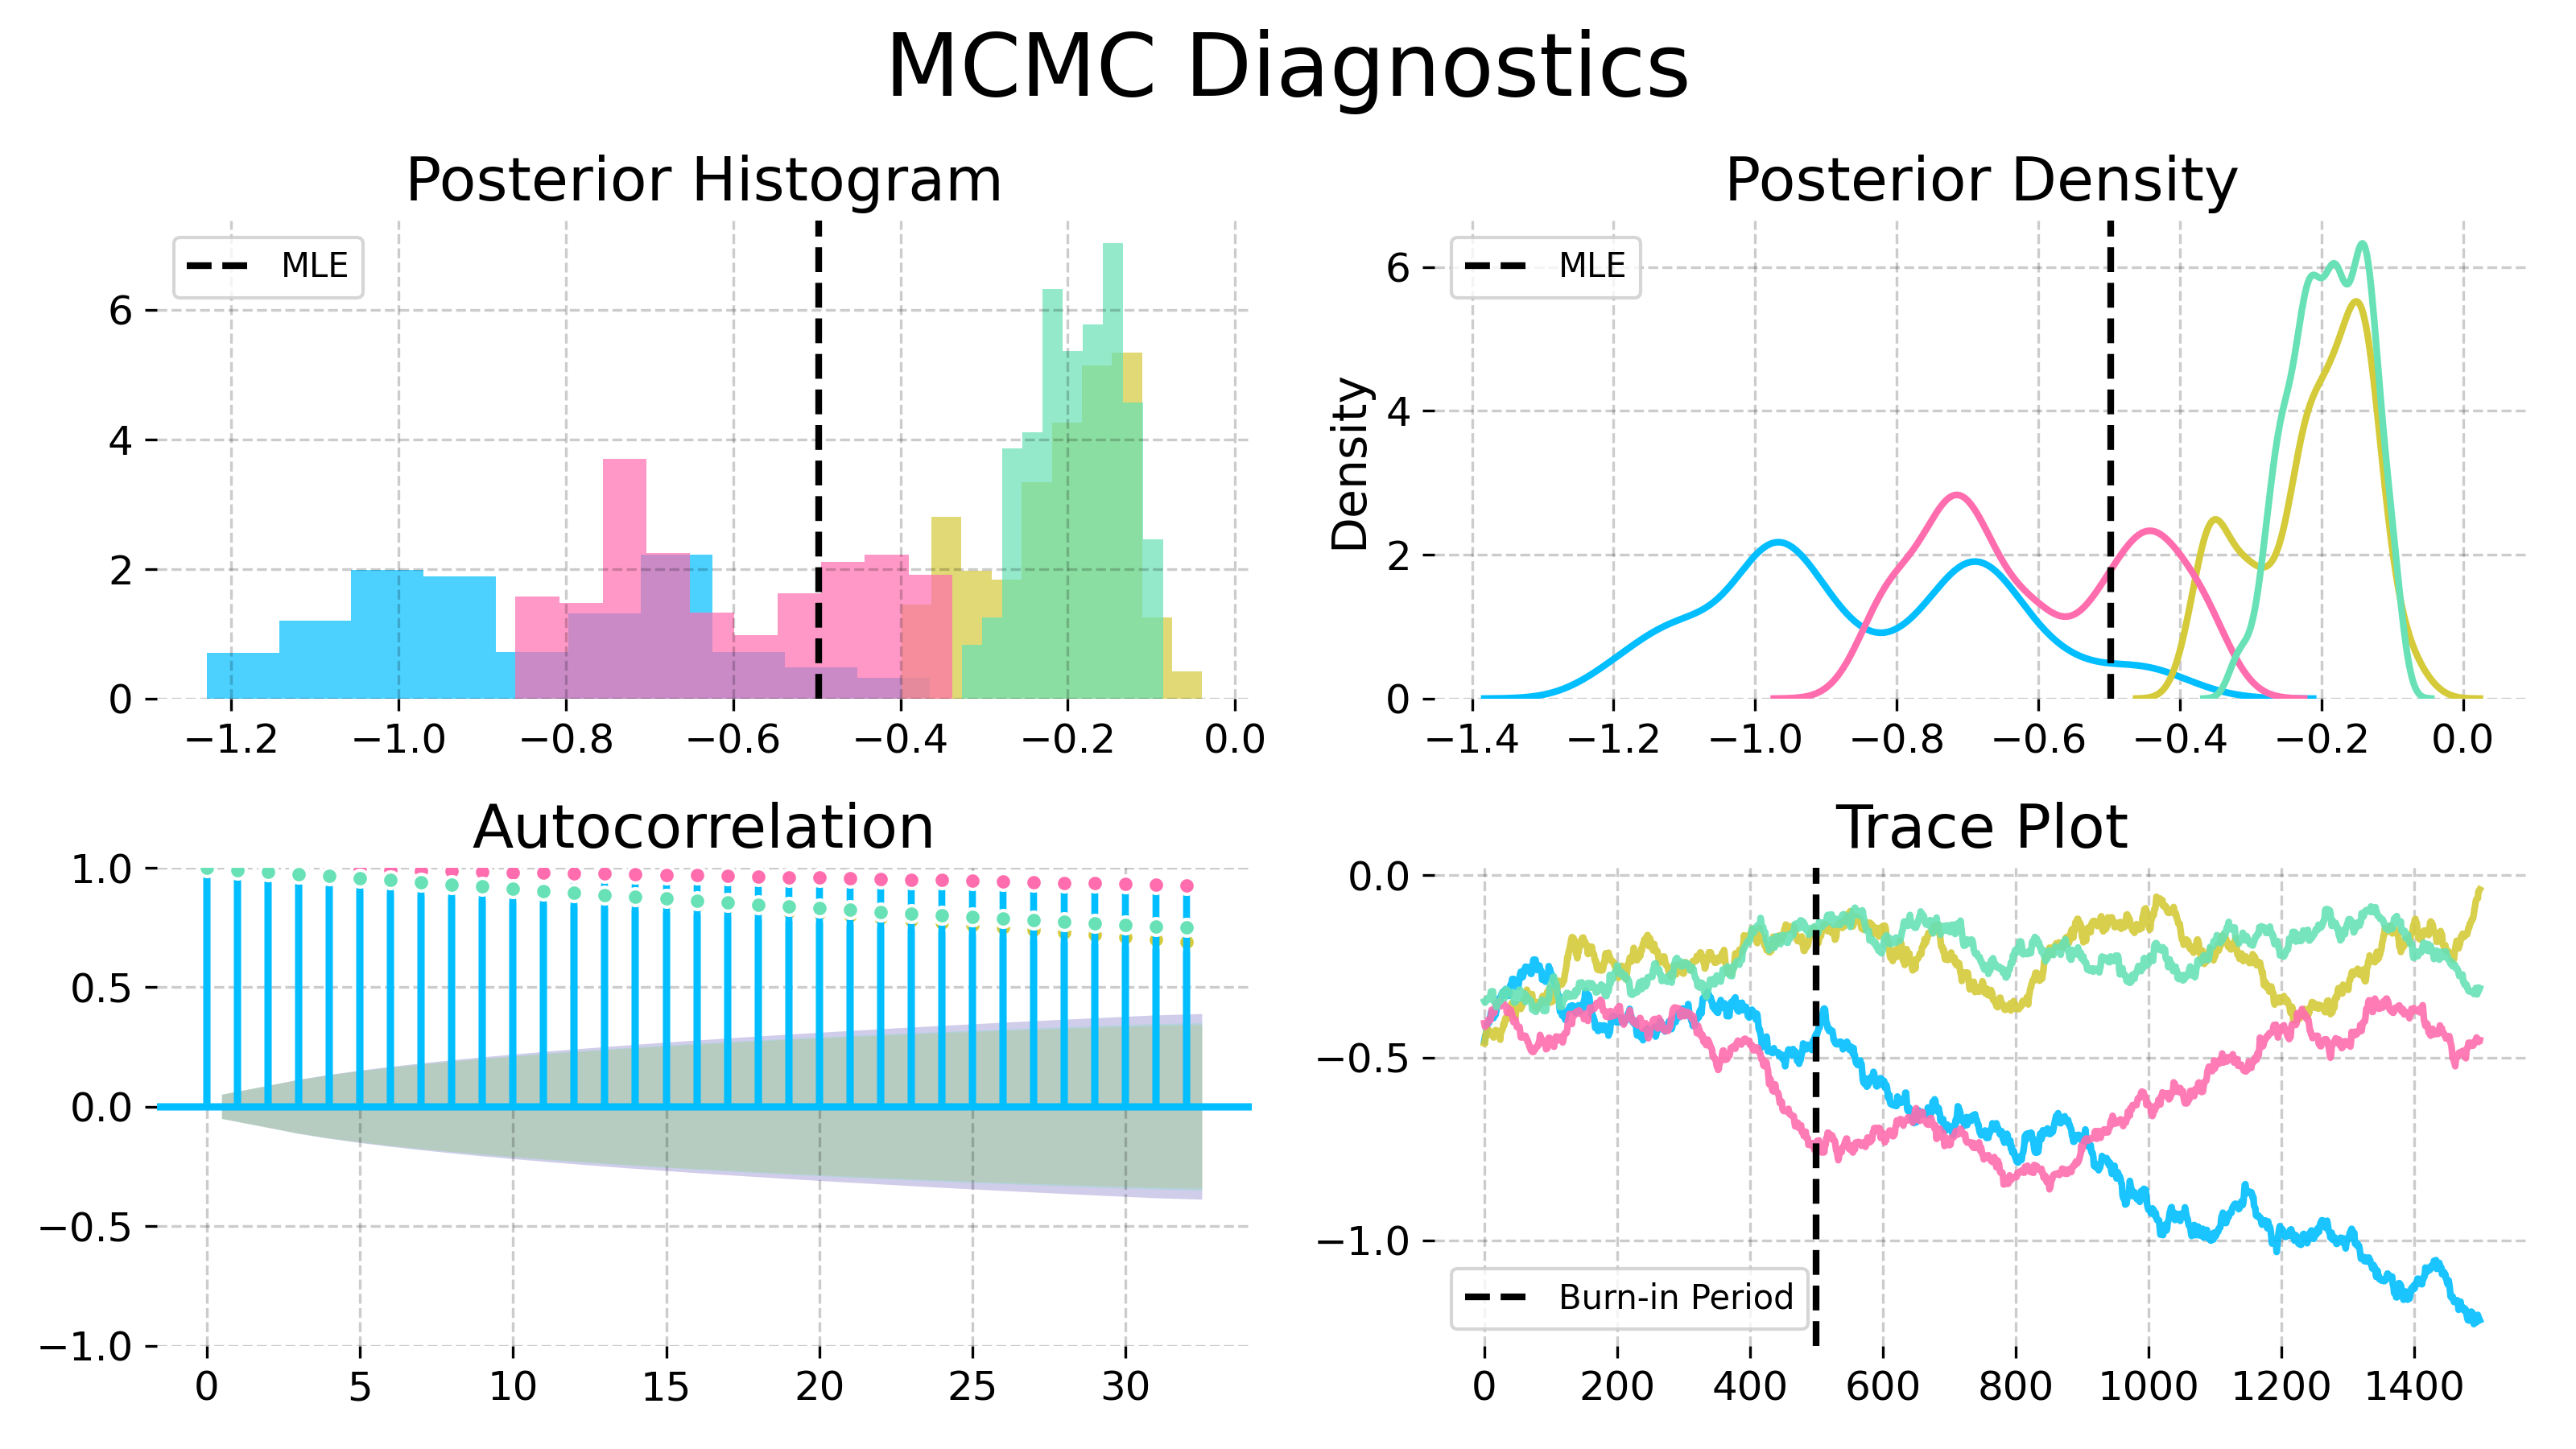
\includegraphics[width=\textwidth/\real{1.3}]{imgs/pmcmc/mh.png}
\caption{
  Convergence diagnostics for the Metropolis-Hastings variant particle MCMC with the random walk proposal and an informative empirical prior from IF2, on the trend parameter in the Dhaka cholera model of \cite{king08}.
  The poor convergence shown here, using an MCMC algorithm that does not have access to derivatives, contrasts with Fig.~{\refFigNutsEb} in the main text.
}
    \label{fig:mh}
\end{figure}
\FloatBarrier

%\newpage

\begin{figure}[H]
    \centering
    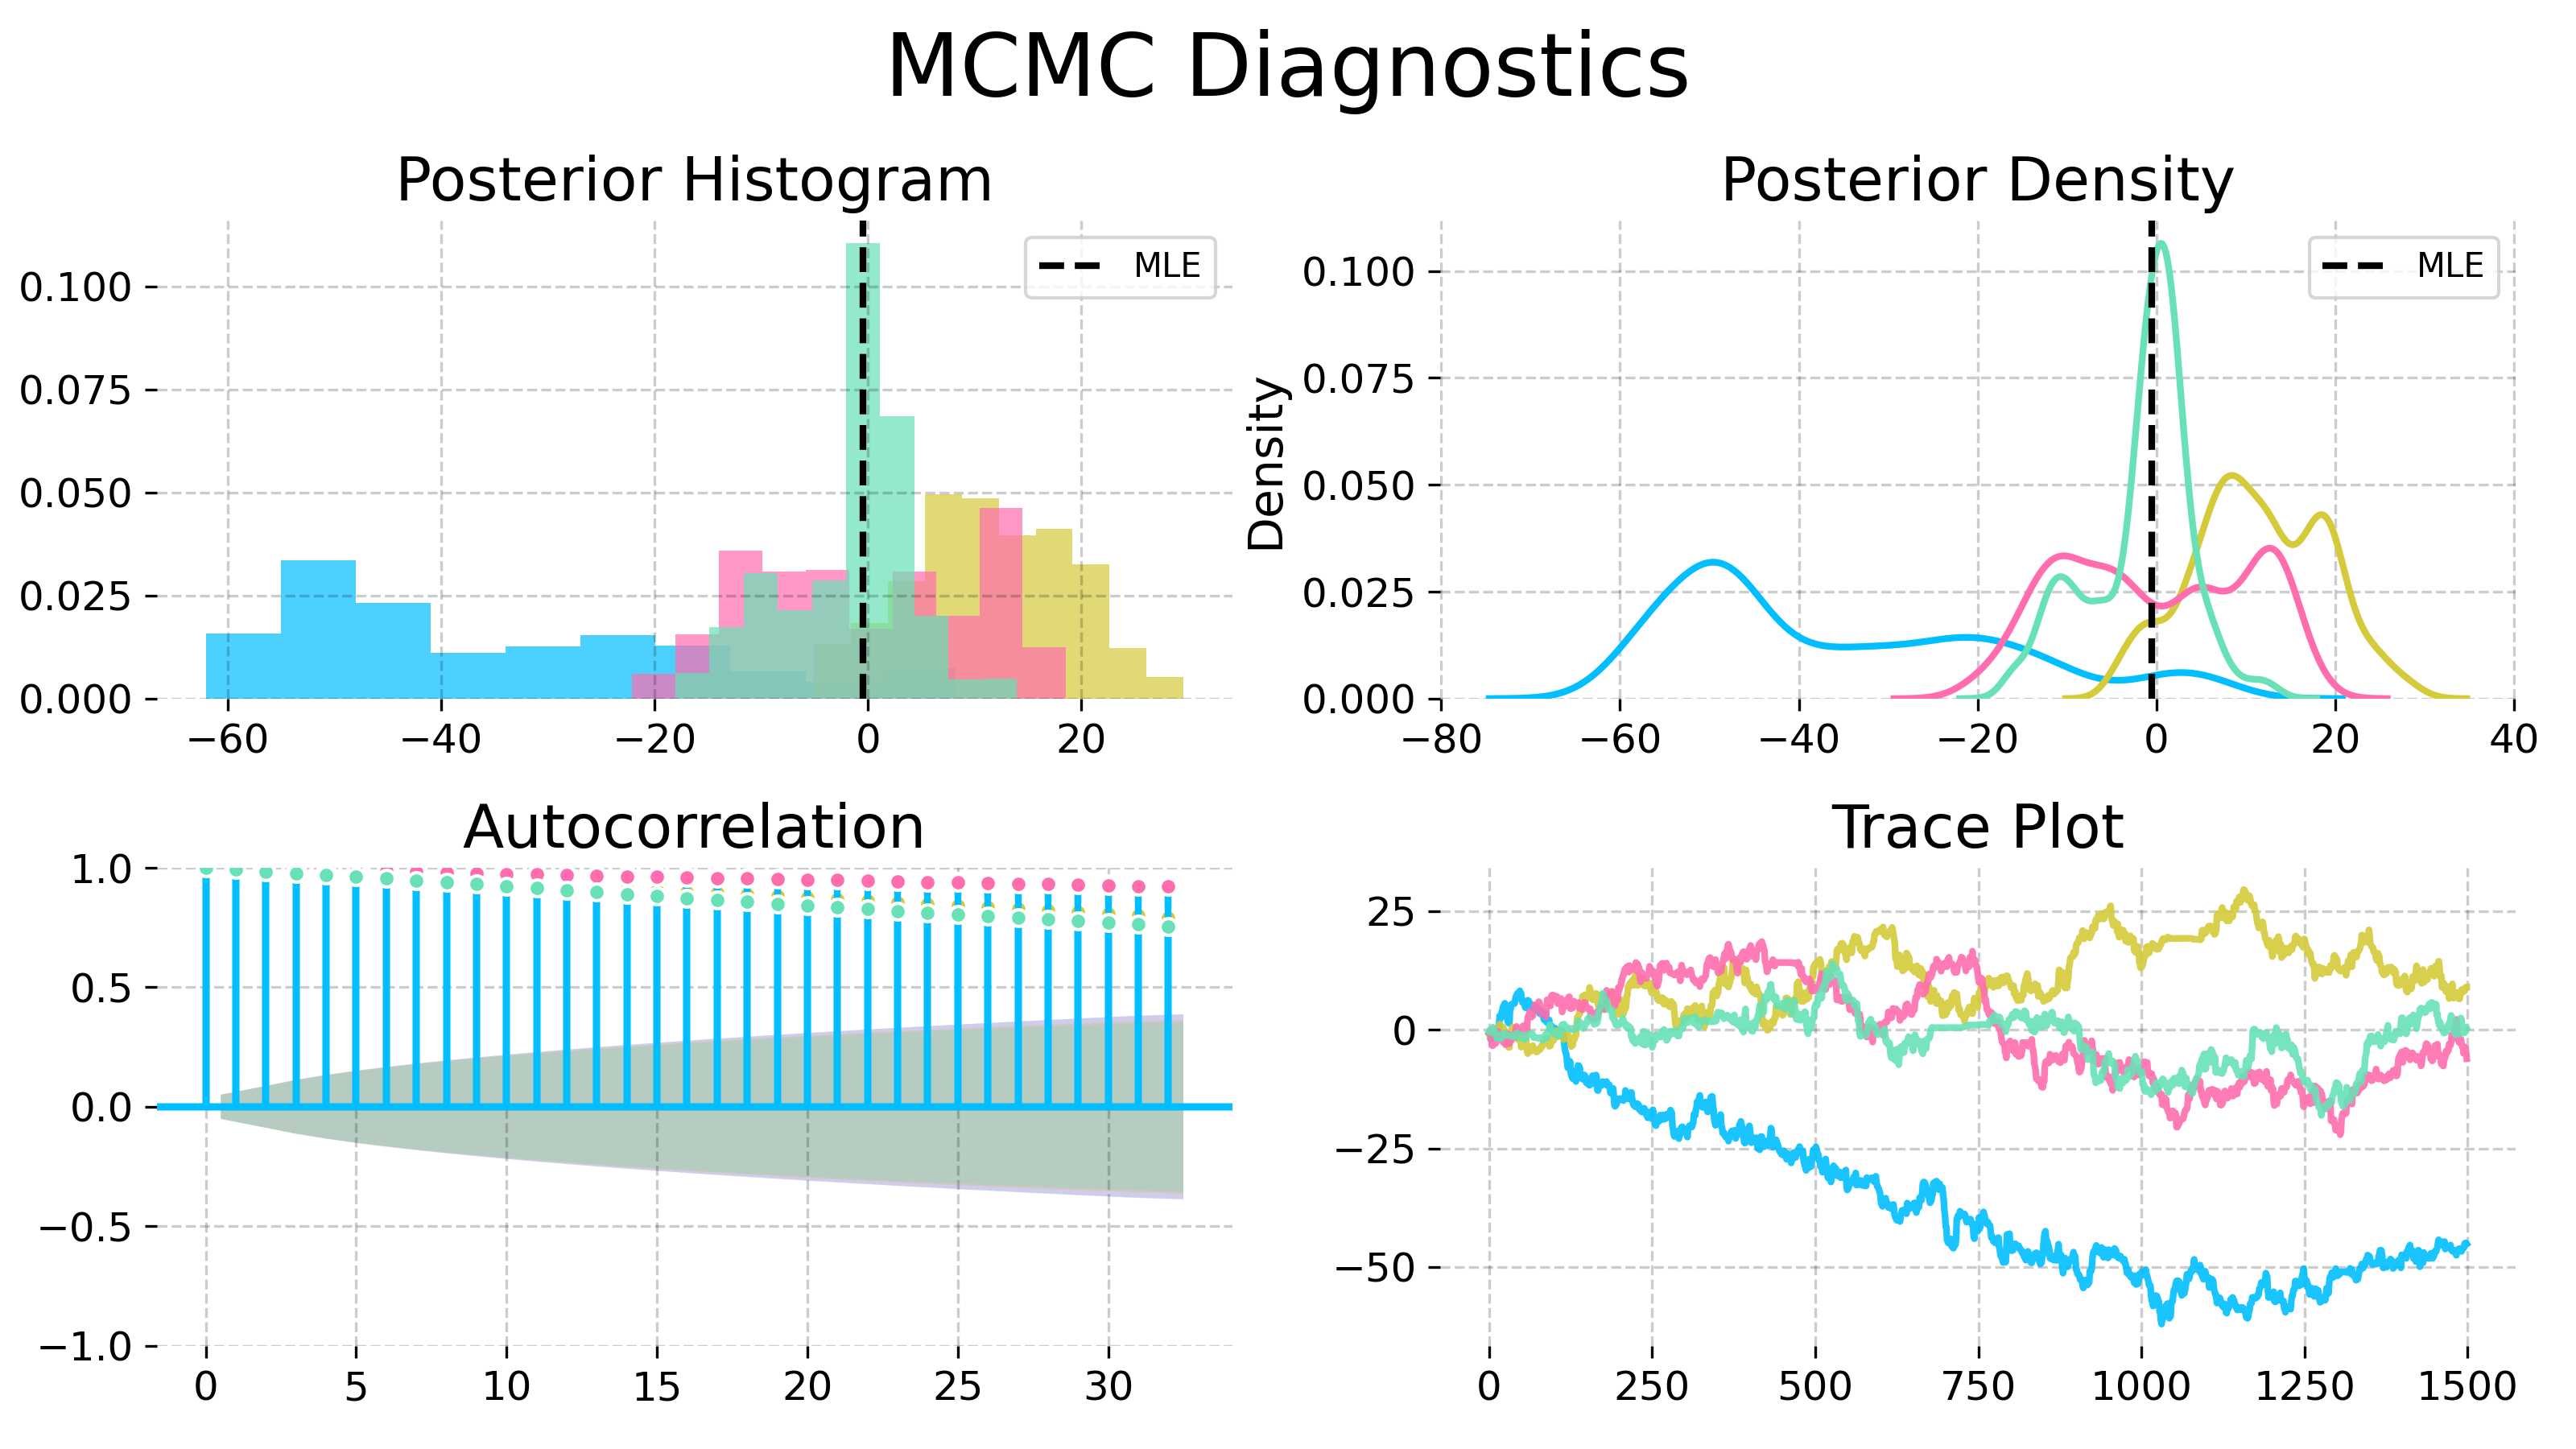
\includegraphics[width=\textwidth/\real{1.3}]{imgs/pmcmc/nuts.png}
    \caption{Convergence diagnostics for a No-U-Turn Sampler (NUTS) with uniform priors on a compact set, on the trend parameter in the Dhaka cholera model of \cite{king08}. The NUTS sampler explores more of the posterior than the Metropolis-Hastings sampler, but fails to converge quickly.
      This poor convergence, compared with Fig.~{\refFigNutsEb} in the main text, demonstrates the value of the empirical prior for obtaining successful convergence.
}
    \label{fig:nuts}
\end{figure}
\FloatBarrier
\newpage

\begin{figure}[H]
    \centering\
    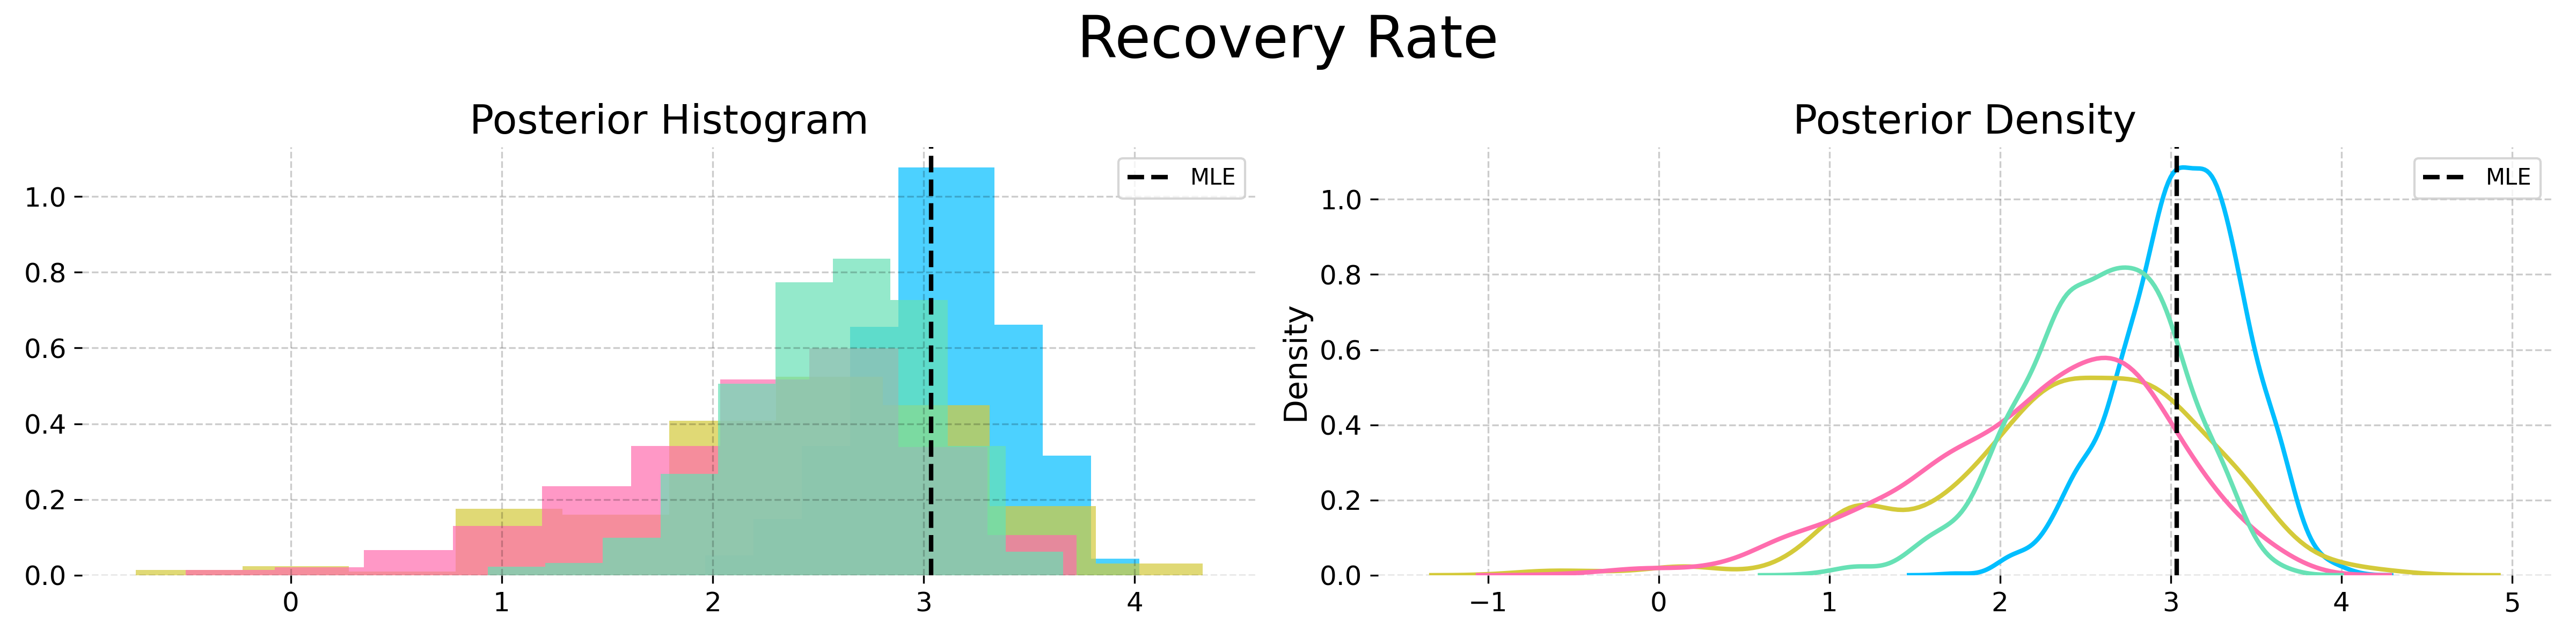
\includegraphics[scale=0.30]{imgs/pmcmc/nuts_eb/Recovery_Rate.png}
    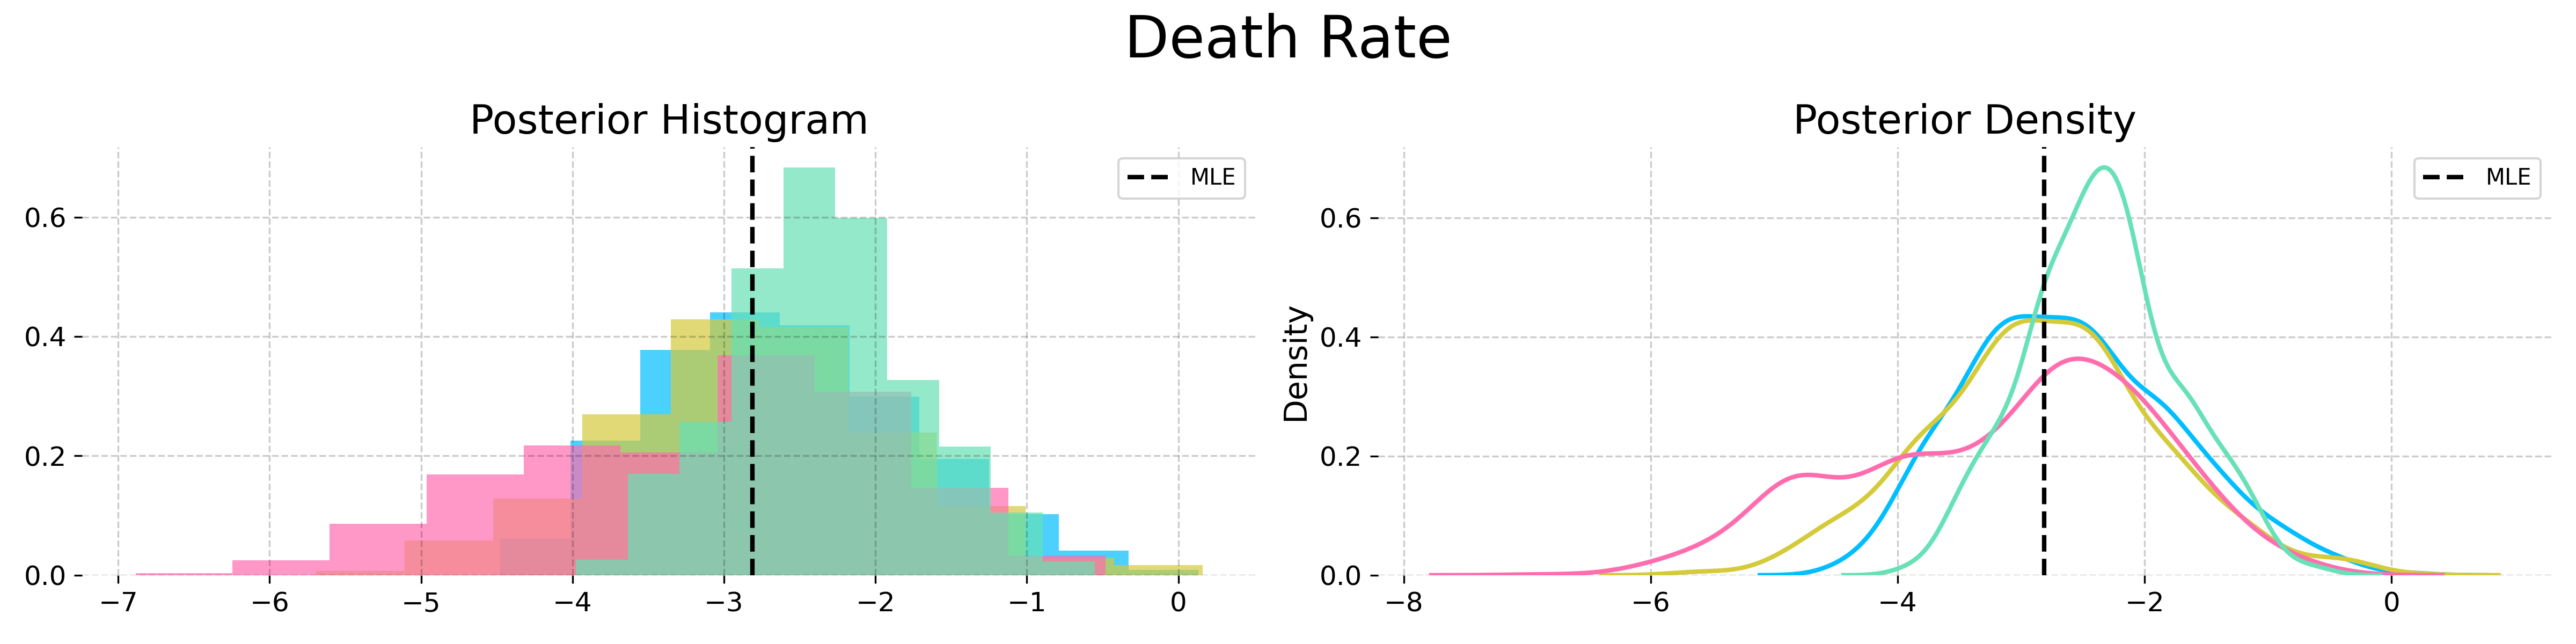
\includegraphics[scale=0.30]{imgs/pmcmc/nuts_eb/Death_Rate.png}
    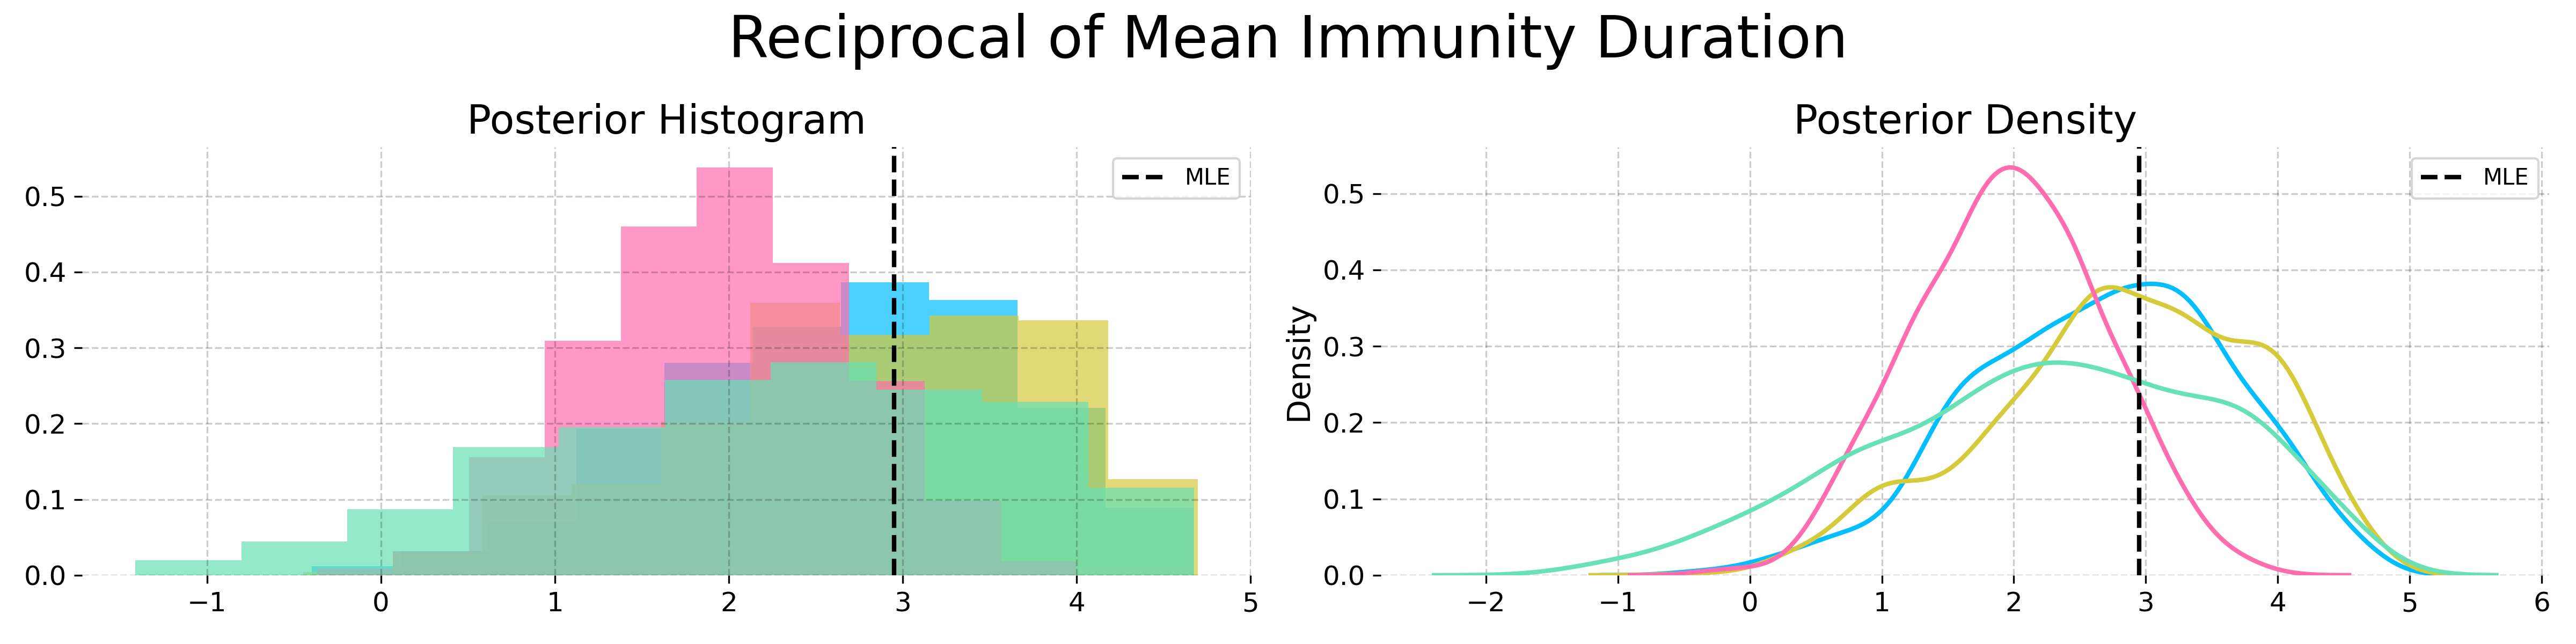
\includegraphics[scale=0.30]{imgs/pmcmc/nuts_eb/Reciprocal_of_Mean_Immunity_Duration.png}
    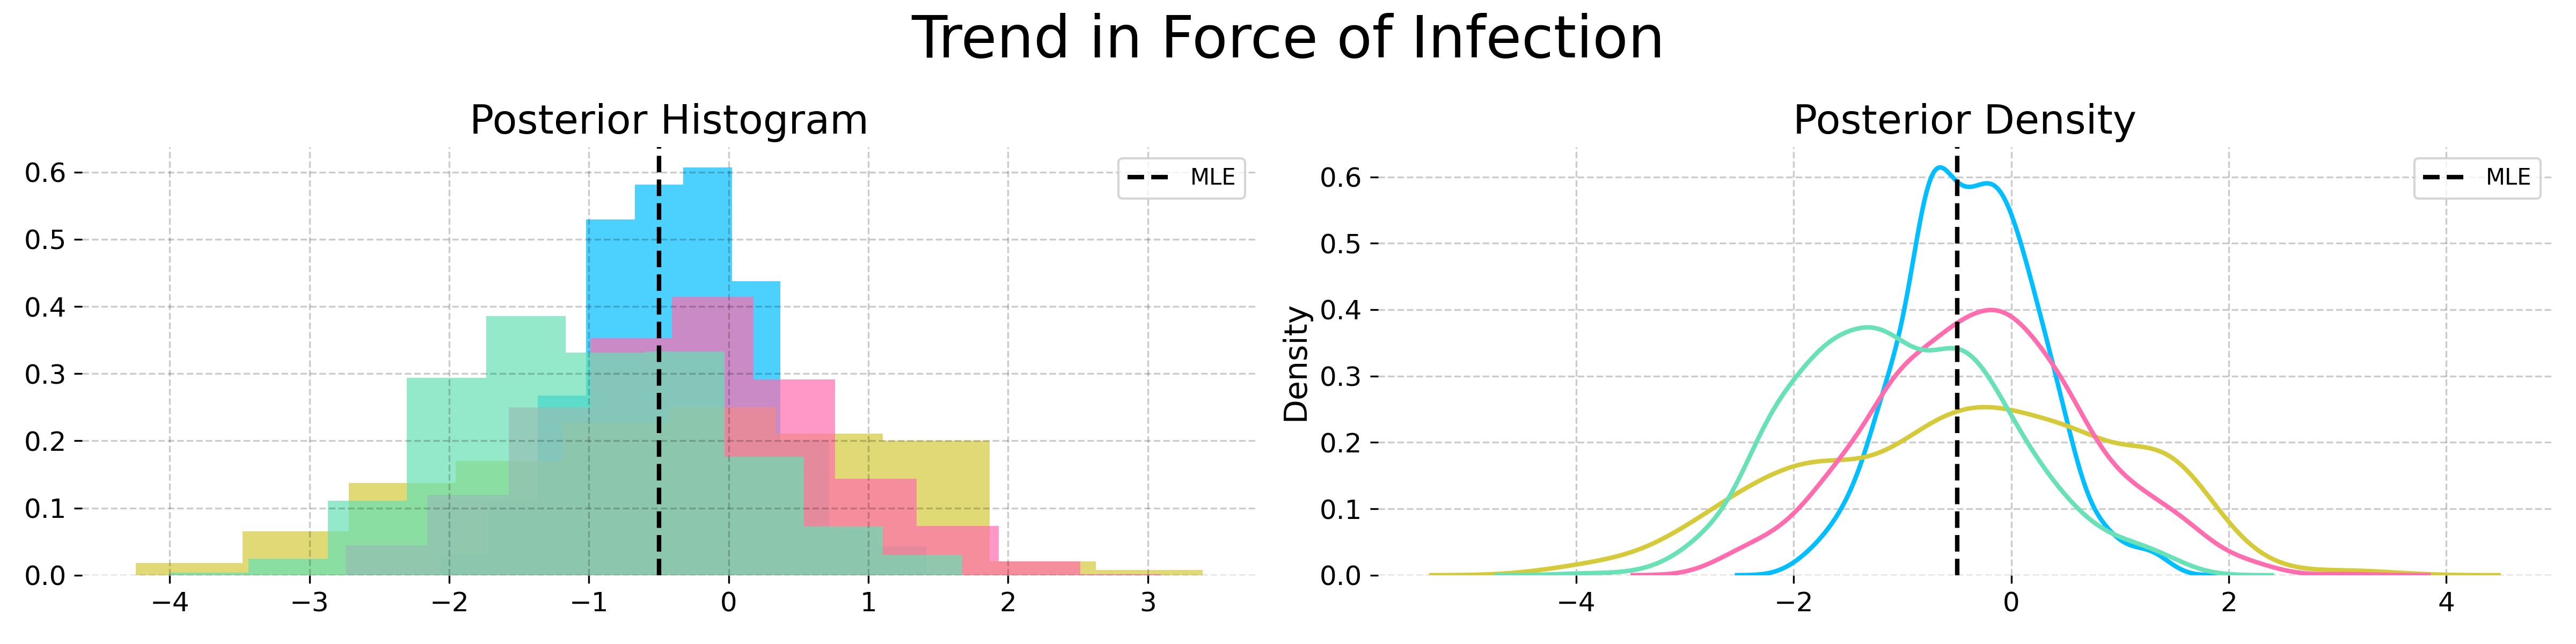
\includegraphics[scale=0.30]{imgs/pmcmc/nuts_eb/Trend_in_Force_of_Infection.png}
    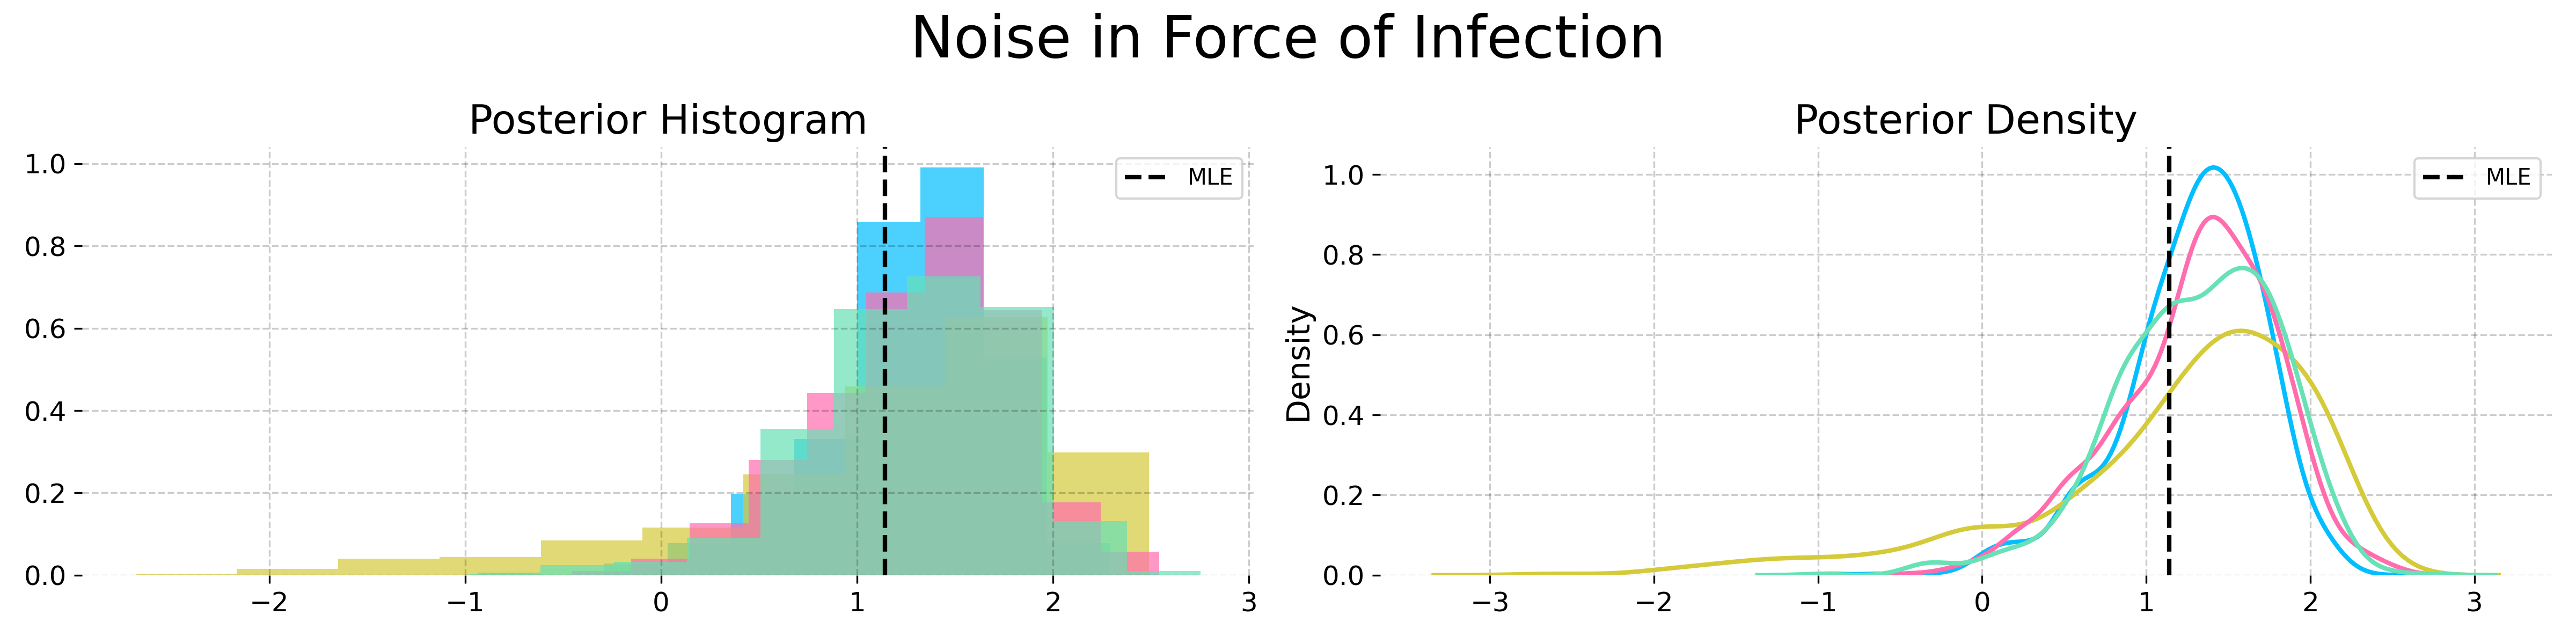
\includegraphics[scale=0.30]{imgs/pmcmc/nuts_eb/Noise_in_Force_of_Infection.png}
    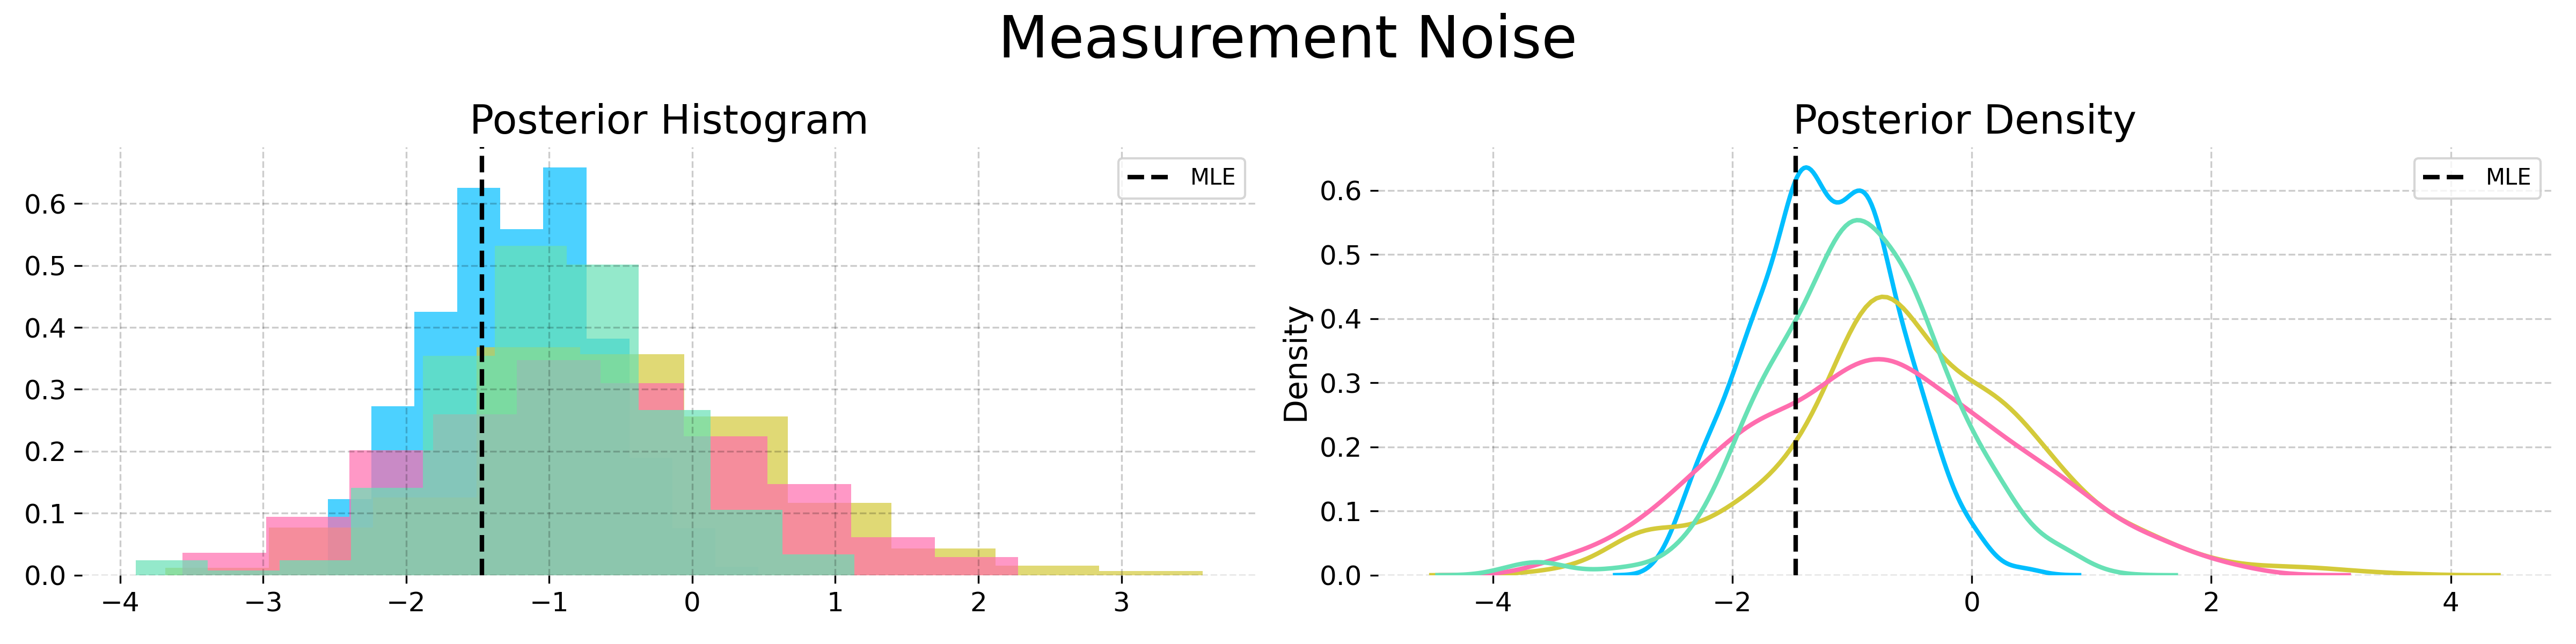
\includegraphics[scale=0.30]{imgs/pmcmc/nuts_eb/Measurement_Noise.png}
    \caption{Posterior estimates from NUTS powered by MOP-$\alpha$ with the informative nonparametric empirical prior obtained from a kernel density estimator on the IF2 parameter cloud. The posterior estimates from each chain are largely in agreement.}
    \label{fig:posteriors}
\end{figure}

\FloatBarrier
\newpage


\section{Justification for the Choice of Baseline Comparisons}

The reasoning we use in the main text to support the magnitude of our contribution is as follows: (i) iterated filtering methods are the current state of the art, and have been for a decade; (ii) we have demonstrated a substantial advance over iterated filtering.
The main text focuses on demonstrating (ii), while supporting (i) via references.
Listing a few references amounts only to anecdotal evidence, which is not sufficient to persuade someone properly skeptical about the claim.
Therefore, this supplement provides an additional quantitative evaluation.

We count the number of papers published in three top scientific journals ({\it Science}, {\it Nature}, and {\it Proceedings of the National Academy of Sciences of the USA (PNAS)}) that carry out statistical inference for partially observed nonlinear non-Gaussian stochastic dynamic models to address a scientific question by fitting mechanistic models to time series data.
For all methods, papers in these high-profile journals are expected to represent only be the tip of the iceberg, but this count provides a concrete measure of the capability of the methods to handle world-class scientific inference problems.
We could have considered additional journals, but the three we chose are undoubtedly prestigious and their scope covers the full range of scientific endeavor so there is less room for subfield bias.
For iterated filtering, our high-impact application count gives the following:
\begin{enumerate*}
  % \item \citet{trevisin23} % this uses pomp for a simulator
\item \citet{he23}\inlineItemSep
  % \item \citet{griffiths23} % this uses pfilter but not if2
  % \item \citet{gokhale23} % uses pomp for trajectory matching
\item \citet{fox22}\inlineItemSep
\item \citet{subramanian21}\inlineItemSep
  \item \citet{pei21}\inlineItemSep
  \item \citet{li20}\inlineItemSep
  %  \item \citet{borchering21} % uses pomp for a simulator
  \item \citet{giezendanner20}\inlineItemSep
\item \citet{wale19}\inlineItemSep
  % \item \citet{decelles19} % uses pomp for trajectory matching
\item \citet{pons-salort18}\inlineItemSep
\item \citet{ranjeva17}\inlineItemSep
\item \citet{martinez16-pnas} \inlineItemSep
\item \citet{becker16}\inlineItemSep
\item \citet{bakker16}\inlineItemSep
\item \citet{laneri15}\inlineItemSep
\item \citet{blake14}\inlineItemSep
\item \citet{blackwood13}\inlineItemSep
\item \citet{blackwood13b}\inlineItemSep
\item \citet{king08}\inlineItemSep
\end{enumerate*}

A referee advised consideration of an alternative approach by \citet{gu98} that we found to have a  high-impact application count of zero, via Google Scholar.

A referee also recommended comparison with \citet{lindsten14}, for which the high-impact application count is also zero.
\citet{lindsten14} has been employed once in {\it Nature Communications} \citep{calafat18} though that journal did not quite make it onto our elite list.
We also found five applications of iterated filtering in {\it Nature Communications} \citep{ranjeva19,rodo21,santos22,briga24,perez25}.
There is a paper in the Statistics section of {\it PNAS} by \citet{wang22} that demonstrates the method of \citet{lindsten14}, but here we are counting the demonstrated ability of the methodology to generate high-profile scientific papers, not statistical methodology papers.
Otherwise, we would also count \citet{ionides06-pnas} and \citet{ionides15} for iterated filtering. 

This reasoning supports iterated filtering as an empirically justified point of reference, in preference to the approaches of \citet{lindsten14} and \citet{gu98}.
Further, the method of \citet{lindsten14} does not have the plug-and-play property so it cannot readily be applied to our example.
The method of \citet{gu98} would have to be combined with an approach such as \citet{andrieu10} that has known scalability problems.
Therefore, we focus on comparing with iterated filtering and we do not provide a comparison with \citet{lindsten14} or \citet{gu98}.

Benchmark tasks are invaluable for making progress on challenging problems \citep{donoho17}.
The Dhaka cholera data and model have served as such a benchmark since its introduction by \citet{king08}.
Other papers testing methods on this example include \citet{ionides15,fasiolo16,wycoff26}.
Thus, our test is established as a demanding inference problem that challenges the best available methods.
We note that this benchmark challenge contains various difficulties that arise commonly in scientific inquiry but are absent from simple SIR models such as the simulation study considered by \citet{lindsten14}.
Ability to accommodate such features is critical for the methodology to be effective for scientific inquiry.

Iterated filtering has recently been used as a benchmark for new POMP model methodology by \citet{whitehouse23}.
This analysis presented numerical results that claimed to beat iterated filtering, but was subsequently found to contain numerical errors.
Corrected results are favorable for iterated filtering methods \citep{hao24-arxiv,whitehouse25-correction,he25}.

Recent results of \citet{chen25} have extended the previous theoretical understanding of iterated filtering.
The ongoing study of iterated filtering as a state-of-the-art approach to inference for POMP models gives additional support for our decision to use iterated filtering as a benchmark for our new methodology.

\section{Algorithmic Parameters}
\label{appendix:algparams}

We include the full set of algorithmic parameters used for the Dhaka results in Table~\ref{table:algparams}. 
The warm start iterations are IF2 iterations, which are followed by gradient descent (GD) iterations when using IFAD. 
The IF2 cooling rate is the fractional reduction in the parameter perturbations over 50 iterations, so that a cooling rate of 0.5 corresponds to approximately 1\% cooling per iteration.
The random walk standard deviation (RWSD) scales the noise added at each filtering step to each regular parameter.
Initial value parameters (IVPs), that affect the value of the latent process only at time $t_0$, are treated differently: they are perturbed only at time $t_0$, with a larger RWSD. 
Parameters are transformed to a unit scale, for example by taking logarithms or a logistic transformation, so that a single RWSD value works for all parameters.

\begin{table}[H]
\centering
\begin{tabular}{p{4.5cm}cccc}
\toprule
\textbf{Hyperparameter} & \textbf{Standard IF2} & \textbf{IFAD-0} & \textbf{IFAD-0.97} & \textbf{IFAD-1} \\
\midrule
Number of Particles ($J$) & 5,000 & 5,000 & 5,000 & 5,000 \\
Warm-start Iterations & 650 & 60 & 175 & 60 \\
GD Iterations & --- & 225 & 175 & 225 \\
IF2 Cooling Rate & 0.8 & 0.5 & 0.5 & 0.5 \\
Initial RWSD & 0.02 & 0.02 & 0.02 & 0.02 \\
Initial RWSD (IVPs) & 0.16 & 0.16 & 0.16 & 0.16 \\
Gradient Optimizer & --- & Adam & Adam & Adam \\
Momentum ($\beta_1$) & --- & 0.0 & 0.9 & 0.9 \\
LR Schedule & --- & Cosine Decay & Cosine Decay & Cosine Decay \\
Initial LR ($\eta_0$) & --- & 0.1 & 0.1 & 0.1 \\
Warm-up Steps & --- & 10 & 10 & 10 \\
Eval. Particles / Reps & 5,000 / 36 & 5,000 / 36 & 5,000 / 36 & 5,000 / 36 \\
\bottomrule
\end{tabular}
\caption{Algorithmic parameters for the global search benchmarking on the Dhaka cholera model.}
\label{table:algparams}
\end{table}

Following some experimentation, IFAD was implemnenteed by plugging the DMOP gradient estimate into the Adam optimizer \citep{kingma14arxiv}.
The momentum parameter in Adam was turned off for IFAD-0, since this low-variance estimate did not reqquire it.
Decreasing the learning rate (LR) was found to be helpful, and we selected the commonly used cosine decay.
Warm-up steps were taken with Adam to stabilize its initial performance and avoid noisy 


\bibliography{bib-ifad}


\end{document}
